\documentclass[twoside]{book}

% Packages required by doxygen
\usepackage{fixltx2e}
\usepackage{calc}
\usepackage{doxygen}
\usepackage{graphicx}
\usepackage[utf8]{inputenc}
\usepackage{makeidx}
\usepackage{multicol}
\usepackage{multirow}
\PassOptionsToPackage{warn}{textcomp}
\usepackage{textcomp}
\usepackage[nointegrals]{wasysym}
\usepackage[table]{xcolor}

% Font selection
\usepackage[T1]{fontenc}
\usepackage{mathptmx}
\usepackage[scaled=.90]{helvet}
\usepackage{courier}
\usepackage{amssymb}
\usepackage{sectsty}
\renewcommand{\familydefault}{\sfdefault}
\allsectionsfont{%
  \fontseries{bc}\selectfont%
  \color{darkgray}%
}
\renewcommand{\DoxyLabelFont}{%
  \fontseries{bc}\selectfont%
  \color{darkgray}%
}
\newcommand{\+}{\discretionary{\mbox{\scriptsize$\hookleftarrow$}}{}{}}

% Page & text layout
\usepackage{geometry}
\geometry{%
  a4paper,%
  top=2.5cm,%
  bottom=2.5cm,%
  left=2.5cm,%
  right=2.5cm%
}
\tolerance=750
\hfuzz=15pt
\hbadness=750
\setlength{\emergencystretch}{15pt}
\setlength{\parindent}{0cm}
\setlength{\parskip}{0.2cm}
\makeatletter
\renewcommand{\paragraph}{%
  \@startsection{paragraph}{4}{0ex}{-1.0ex}{1.0ex}{%
    \normalfont\normalsize\bfseries\SS@parafont%
  }%
}
\renewcommand{\subparagraph}{%
  \@startsection{subparagraph}{5}{0ex}{-1.0ex}{1.0ex}{%
    \normalfont\normalsize\bfseries\SS@subparafont%
  }%
}
\makeatother

% Headers & footers
\usepackage{fancyhdr}
\pagestyle{fancyplain}
\fancyhead[LE]{\fancyplain{}{\bfseries\thepage}}
\fancyhead[CE]{\fancyplain{}{}}
\fancyhead[RE]{\fancyplain{}{\bfseries\leftmark}}
\fancyhead[LO]{\fancyplain{}{\bfseries\rightmark}}
\fancyhead[CO]{\fancyplain{}{}}
\fancyhead[RO]{\fancyplain{}{\bfseries\thepage}}
\fancyfoot[LE]{\fancyplain{}{}}
\fancyfoot[CE]{\fancyplain{}{}}
\fancyfoot[RE]{\fancyplain{}{\bfseries\scriptsize Generated on Tue Jan 20 2015 15\+:03\+:29 for Fact\+Dev by Doxygen }}
\fancyfoot[LO]{\fancyplain{}{\bfseries\scriptsize Generated on Tue Jan 20 2015 15\+:03\+:29 for Fact\+Dev by Doxygen }}
\fancyfoot[CO]{\fancyplain{}{}}
\fancyfoot[RO]{\fancyplain{}{}}
\renewcommand{\footrulewidth}{0.4pt}
\renewcommand{\chaptermark}[1]{%
  \markboth{#1}{}%
}
\renewcommand{\sectionmark}[1]{%
  \markright{\thesection\ #1}%
}

% Indices & bibliography
\usepackage{natbib}
\usepackage[titles]{tocloft}
\setcounter{tocdepth}{3}
\setcounter{secnumdepth}{5}
\makeindex

% Hyperlinks (required, but should be loaded last)
\usepackage{ifpdf}
\ifpdf
  \usepackage[pdftex,pagebackref=true]{hyperref}
\else
  \usepackage[ps2pdf,pagebackref=true]{hyperref}
\fi
\hypersetup{%
  colorlinks=true,%
  linkcolor=blue,%
  citecolor=blue,%
  unicode%
}

% Custom commands
\newcommand{\clearemptydoublepage}{%
  \newpage{\pagestyle{empty}\cleardoublepage}%
}


%===== C O N T E N T S =====

\begin{document}

% Titlepage & ToC
\hypersetup{pageanchor=false,
             bookmarks=true,
             bookmarksnumbered=true,
             pdfencoding=unicode
            }
\pagenumbering{roman}
\begin{titlepage}
\vspace*{7cm}
\begin{center}%
{\Large Fact\+Dev \\[1ex]\large 0.\+1 }\\
\vspace*{1cm}
{\large Generated by Doxygen 1.8.8}\\
\vspace*{0.5cm}
{\small Tue Jan 20 2015 15:03:29}\\
\end{center}
\end{titlepage}
\clearemptydoublepage
\tableofcontents
\clearemptydoublepage
\pagenumbering{arabic}
\hypersetup{pageanchor=true}

%--- Begin generated contents ---
\chapter{Fact\+Dev documentation}
\label{index}\hypertarget{index}{}This website contains the documentation of Fact\+Dev, a billings and quotes software.

\section*{Team}

F\+A\+C\+T team is a team for Universitiy Project. Members of this team are \+:
\begin{DoxyItemize}
\item Florent Berbie (\href{https://github.com/KraTuX31 KraTuX31}{\tt Kra\+Tu\+X31})
\item Antoine de Roquemaurel (\href{https://github.com/aroquemaurel}{\tt aroquemaurel})
\item Cédric Rohaut (\href{https://github.com/Oxynos}{\tt Oxynos})
\item Manantsoa Andriamihary Razanajatovo (\href{https://github.com/manantsoa}{\tt manantsoa})
\end{DoxyItemize}

For more informations, you can go to \href{http://fact-team.github.io}{\tt http\+://fact-\/team.\+github.\+io}.

\section*{What is Fact\+Dev ?}

 

Fact\+Dev is a software for quotes and billings developped by F\+A\+C\+T team for university project in Toulouse I\+I\+I University – Paul Sabatier.

This software is developped with C++ and Qt framework, and there is differents features \+:
\begin{DoxyItemize}
\item Customers database
\item Differents projects for customers
\item Quotes
\item Billings
\end{DoxyItemize}

\section*{Documentation}

You can access to the documentation generated by Doxygen here \+:
\begin{DoxyItemize}
\item \href{http://fact-team.github.io/doc/html/index.html}{\tt H\+T\+M\+L Documentation}
\item \href{http://fact-team.github.io/doc/latex/refman.pdf}{\tt P\+D\+F Documentation}
\end{DoxyItemize}

\section*{Installation and using}


\begin{DoxyItemize}
\item \href{http://fact-team.github.io/doc/usermanual.pdf}{\tt User Manual} 
\end{DoxyItemize}
\chapter{Q\+Test\+Runner}
\label{dc/d04/md_tests_QTestRunner_README}
\hypertarget{dc/d04/md_tests_QTestRunner_README}{}
A repo for Increase Q\+Test productivity

Thanks to \href{https://marcoarena.wordpress.com/2012/06/23/increase-your-qtest-productivity/}{\tt https\+://marcoarena.\+wordpress.\+com/2012/06/23/increase-\/your-\/qtest-\/productivity/} ! \begin{quote}
The Q\+Test\+Lib framework is a tool for unit testing Qt based applications and libraries. I find it precious and simple to use, though it lacks some important features, supported, for example, by G\+Test. I’m not talking about mocking – for this you generally need an out-\/and-\/out framework (like G\+Mock) – instead, I’m referring to simple things like fast deploying. Suppose you have written a test class like this\+: \end{quote}


This repo contains only the code in this article. 
\chapter{Hierarchical Index}
\section{Class Hierarchy}
This inheritance list is sorted roughly, but not completely, alphabetically\-:\begin{DoxyCompactList}
\item \contentsline{section}{Mustache\-:\-:Context}{\pageref{d7/d34/classMustache_1_1Context}}{}
\begin{DoxyCompactList}
\item \contentsline{section}{Mustache\-:\-:Qt\-Variant\-Context}{\pageref{d5/d8b/classMustache_1_1QtVariantContext}}{}
\begin{DoxyCompactList}
\item \contentsline{section}{Counter\-Context}{\pageref{db/da6/classCounterContext}}{}
\item \contentsline{section}{Counter\-Context}{\pageref{db/da6/classCounterContext}}{}
\end{DoxyCompactList}
\end{DoxyCompactList}
\item \contentsline{section}{Contributory\-List\-Test}{\pageref{d4/de2/classContributoryListTest}}{}
\item \contentsline{section}{Databases\-:\-:Database}{\pageref{dd/db0/classDatabases_1_1Database}}{}
\begin{DoxyCompactList}
\item \contentsline{section}{Databases\-:\-:Billing\-Database}{\pageref{df/df8/classDatabases_1_1BillingDatabase}}{}
\item \contentsline{section}{Databases\-:\-:Contributory\-Database}{\pageref{dc/da5/classDatabases_1_1ContributoryDatabase}}{}
\item \contentsline{section}{Databases\-:\-:Customer\-Database}{\pageref{d8/d7e/classDatabases_1_1CustomerDatabase}}{}
\item \contentsline{section}{Databases\-:\-:Project\-Database}{\pageref{d7/d39/classDatabases_1_1ProjectDatabase}}{}
\item \contentsline{section}{Databases\-:\-:Rate\-Database}{\pageref{d9/d21/classDatabases_1_1RateDatabase}}{}
\item \contentsline{section}{Databases\-:\-:User\-Database}{\pageref{d0/d33/classDatabases_1_1UserDatabase}}{}
\end{DoxyCompactList}
\item \contentsline{section}{Utils\-:\-:Directories}{\pageref{d8/d40/classUtils_1_1Directories}}{}
\item exception\begin{DoxyCompactList}
\item \contentsline{section}{Exceptions\-:\-:Db\-Exception}{\pageref{d4/de4/classExceptions_1_1DbException}}{}
\end{DoxyCompactList}
\item \contentsline{section}{Exceptions\-:\-:File\-Exception}{\pageref{d9/d57/classExceptions_1_1FileException}}{}
\item \contentsline{section}{Generator}{\pageref{d9/d12/classGenerator}}{}
\item \contentsline{section}{Utils\-:\-:Hierarchical\-System}{\pageref{d1/de0/classUtils_1_1HierarchicalSystem}}{}
\item \contentsline{section}{Gui\-:\-:Widgets\-:\-:Check\-Fields\-:\-:I\-Check\-Field}{\pageref{d7/d93/classGui_1_1Widgets_1_1CheckFields_1_1ICheckField}}{}
\begin{DoxyCompactList}
\item \contentsline{section}{Gui\-:\-:Widgets\-:\-:Check\-Fields\-:\-:Check\-Q\-Line\-Edit}{\pageref{d0/d68/classGui_1_1Widgets_1_1CheckFields_1_1CheckQLineEdit}}{}
\begin{DoxyCompactList}
\item \contentsline{section}{Gui\-:\-:Widgets\-:\-:Check\-Fields\-:\-:Check\-Email}{\pageref{d1/d07/classGui_1_1Widgets_1_1CheckFields_1_1CheckEmail}}{}
\item \contentsline{section}{Gui\-:\-:Widgets\-:\-:Check\-Fields\-:\-:Check\-Siret\-Number}{\pageref{db/d94/classGui_1_1Widgets_1_1CheckFields_1_1CheckSiretNumber}}{}
\item \contentsline{section}{Gui\-:\-:Widgets\-:\-:Check\-Fields\-:\-:Check\-Until\-Field}{\pageref{d4/d37/classGui_1_1Widgets_1_1CheckFields_1_1CheckUntilField}}{}
\begin{DoxyCompactList}
\item \contentsline{section}{Gui\-:\-:Widgets\-:\-:Check\-Fields\-:\-:Check\-Fields\-Letters}{\pageref{df/dba/classGui_1_1Widgets_1_1CheckFields_1_1CheckFieldsLetters}}{}
\begin{DoxyCompactList}
\item \contentsline{section}{Gui\-:\-:Widgets\-:\-:Check\-Fields\-:\-:Check\-City}{\pageref{dd/da5/classGui_1_1Widgets_1_1CheckFields_1_1CheckCity}}{}
\item \contentsline{section}{Gui\-:\-:Widgets\-:\-:Check\-Fields\-:\-:Check\-Country}{\pageref{d0/d3f/classGui_1_1Widgets_1_1CheckFields_1_1CheckCountry}}{}
\item \contentsline{section}{Gui\-:\-:Widgets\-:\-:Check\-Fields\-:\-:Check\-Name}{\pageref{da/d67/classGui_1_1Widgets_1_1CheckFields_1_1CheckName}}{}
\end{DoxyCompactList}
\item \contentsline{section}{Gui\-:\-:Widgets\-:\-:Check\-Fields\-:\-:Check\-Phone}{\pageref{da/dc0/classGui_1_1Widgets_1_1CheckFields_1_1CheckPhone}}{}
\item \contentsline{section}{Gui\-:\-:Widgets\-:\-:Check\-Fields\-:\-:Check\-Postal\-Code}{\pageref{df/d31/classGui_1_1Widgets_1_1CheckFields_1_1CheckPostalCode}}{}
\end{DoxyCompactList}
\item \contentsline{section}{Gui\-:\-:Widgets\-:\-:Check\-Fields\-:\-:Check\-Valid\-Field}{\pageref{d8/d6d/classGui_1_1Widgets_1_1CheckFields_1_1CheckValidField}}{}
\end{DoxyCompactList}
\end{DoxyCompactList}
\item \contentsline{section}{Models\-:\-:I\-Model}{\pageref{d0/d9c/classModels_1_1IModel}}{}
\begin{DoxyCompactList}
\item \contentsline{section}{Models\-:\-:Billing}{\pageref{d4/d5c/classModels_1_1Billing}}{}
\item \contentsline{section}{Models\-:\-:Contributory}{\pageref{d5/dd1/classModels_1_1Contributory}}{}
\item \contentsline{section}{Models\-:\-:Customer}{\pageref{db/dd7/classModels_1_1Customer}}{}
\item \contentsline{section}{Models\-:\-:Project}{\pageref{dd/d3f/classModels_1_1Project}}{}
\item \contentsline{section}{Models\-:\-:User}{\pageref{df/d68/classModels_1_1User}}{}
\end{DoxyCompactList}
\item \contentsline{section}{Utils\-:\-:Item\-Type}{\pageref{d5/d7c/classUtils_1_1ItemType}}{}
\item \contentsline{section}{Utils\-:\-:Log}{\pageref{db/db3/classUtils_1_1Log}}{}
\item \contentsline{section}{Parameters}{\pageref{de/d0a/classParameters}}{}
\item \contentsline{section}{Mustache\-:\-:Partial\-Resolver}{\pageref{d0/dce/classMustache_1_1PartialResolver}}{}
\begin{DoxyCompactList}
\item \contentsline{section}{Mustache\-:\-:Partial\-File\-Loader}{\pageref{da/d31/classMustache_1_1PartialFileLoader}}{}
\item \contentsline{section}{Mustache\-:\-:Partial\-Map}{\pageref{dc/d1a/classMustache_1_1PartialMap}}{}
\end{DoxyCompactList}
\item \contentsline{section}{Utils\-:\-:pointers}{\pageref{d4/d7a/classUtils_1_1pointers}}{}
\item \contentsline{section}{Gui\-:\-:Widgets\-:\-:Popup}{\pageref{d4/d2f/classGui_1_1Widgets_1_1Popup}}{}
\item Q\-Abstract\-Table\-Model\begin{DoxyCompactList}
\item \contentsline{section}{Gui\-:\-:Widgets\-:\-:Wdg\-Models\-:\-:Billings\-Table\-Model}{\pageref{dc/d82/classGui_1_1Widgets_1_1WdgModels_1_1BillingsTableModel}}{}
\item \contentsline{section}{Gui\-:\-:Widgets\-:\-:Wdg\-Models\-:\-:Contributories\-Table\-Model}{\pageref{dc/db9/classGui_1_1Widgets_1_1WdgModels_1_1ContributoriesTableModel}}{}
\item \contentsline{section}{Gui\-:\-:Widgets\-:\-:Wdg\-Models\-:\-:Customers\-Table\-Model}{\pageref{d7/d12/classGui_1_1Widgets_1_1WdgModels_1_1CustomersTableModel}}{}
\item \contentsline{section}{Gui\-:\-:Widgets\-:\-:Wdg\-Models\-:\-:Project\-Contributories\-Table\-Model}{\pageref{d9/d71/classGui_1_1Widgets_1_1WdgModels_1_1ProjectContributoriesTableModel}}{}
\item \contentsline{section}{Gui\-:\-:Widgets\-:\-:Wdg\-Models\-:\-:Projects\-Table\-Model}{\pageref{d3/d40/classGui_1_1Widgets_1_1WdgModels_1_1ProjectsTableModel}}{}
\end{DoxyCompactList}
\item Q\-Dialog\begin{DoxyCompactList}
\item \contentsline{section}{Gui\-:\-:Dialogs\-:\-:Add\-Project\-Dialog}{\pageref{de/d36/classGui_1_1Dialogs_1_1AddProjectDialog}}{}
\item \contentsline{section}{Gui\-:\-:Dialogs\-:\-:Add\-Quote\-Dialog}{\pageref{d6/d43/classGui_1_1Dialogs_1_1AddQuoteDialog}}{}
\item \contentsline{section}{Gui\-:\-:Dialogs\-:\-:Dialog\-Add\-Customer}{\pageref{d2/d50/classGui_1_1Dialogs_1_1DialogAddCustomer}}{}
\item \contentsline{section}{Gui\-:\-:Dialogs\-:\-:Message\-Box}{\pageref{d9/d31/classGui_1_1Dialogs_1_1MessageBox}}{}
\item \contentsline{section}{Gui\-:\-:Dialogs\-:\-:User\-Data\-Dialog}{\pageref{d3/d81/classGui_1_1Dialogs_1_1UserDataDialog}}{}
\item \contentsline{section}{Started\-Windows\-Dialog}{\pageref{da/ddc/classStartedWindowsDialog}}{}
\end{DoxyCompactList}
\item Q\-Dock\-Widget\begin{DoxyCompactList}
\item \contentsline{section}{Gui\-:\-:Docks\-:\-:Search\-Dock}{\pageref{de/db4/classGui_1_1Docks_1_1SearchDock}}{}
\end{DoxyCompactList}
\item Q\-Item\-Delegate\begin{DoxyCompactList}
\item \contentsline{section}{Gui\-:\-:Widgets\-:\-:Delegates\-:\-:Combo\-Box\-Delegate}{\pageref{d5/d72/classGui_1_1Widgets_1_1Delegates_1_1ComboBoxDelegate}}{}
\begin{DoxyCompactList}
\item \contentsline{section}{Gui\-:\-:Widgets\-:\-:Delegates\-:\-:Project\-Combo\-Delegate}{\pageref{d6/d93/classGui_1_1Widgets_1_1Delegates_1_1ProjectComboDelegate}}{}
\item \contentsline{section}{Gui\-:\-:Widgets\-:\-:Delegates\-:\-:Unit\-Combo\-Delegate}{\pageref{db/def/classGui_1_1Widgets_1_1Delegates_1_1UnitComboDelegate}}{}
\end{DoxyCompactList}
\item \contentsline{section}{Gui\-:\-:Widgets\-:\-:Delegates\-:\-:Double\-Spin\-Box\-Delegate}{\pageref{da/d53/classGui_1_1Widgets_1_1Delegates_1_1DoubleSpinBoxDelegate}}{}
\end{DoxyCompactList}
\item Q\-Line\-Edit\begin{DoxyCompactList}
\item \contentsline{section}{Gui\-:\-:Widgets\-:\-:Check\-Fields\-:\-:Check\-Q\-Line\-Edit}{\pageref{d0/d68/classGui_1_1Widgets_1_1CheckFields_1_1CheckQLineEdit}}{}
\end{DoxyCompactList}
\item Q\-Main\-Window\begin{DoxyCompactList}
\item \contentsline{section}{Gui\-:\-:Main\-Window}{\pageref{d5/d2f/classGui_1_1MainWindow}}{}
\end{DoxyCompactList}
\item Q\-Map\begin{DoxyCompactList}
\item \contentsline{section}{Models\-:\-:Contributories\-List}{\pageref{d7/d6a/classModels_1_1ContributoriesList}}{}
\end{DoxyCompactList}
\item Q\-Menu\begin{DoxyCompactList}
\item \contentsline{section}{Gui\-:\-:Widgets\-:\-:Customer\-Contextual\-Menu}{\pageref{d8/ded/classGui_1_1Widgets_1_1CustomerContextualMenu}}{}
\end{DoxyCompactList}
\item Q\-Object\begin{DoxyCompactList}
\item \contentsline{section}{Billing\-Database\-Test}{\pageref{d1/db1/classBillingDatabaseTest}}{}
\item \contentsline{section}{Billing\-Model\-Test}{\pageref{dc/d0c/classBillingModelTest}}{}
\item \contentsline{section}{Contributories\-Database\-Test}{\pageref{d8/df7/classContributoriesDatabaseTest}}{}
\item \contentsline{section}{Contributory\-Model\-Test}{\pageref{d5/d97/classContributoryModelTest}}{}
\item \contentsline{section}{Customer\-Database\-Test}{\pageref{d2/d63/classCustomerDatabaseTest}}{}
\item \contentsline{section}{Customer\-Model\-Test}{\pageref{d5/dcd/classCustomerModelTest}}{}
\item \contentsline{section}{Generation}{\pageref{d4/df7/classGeneration}}{}
\item \contentsline{section}{Item\-Type\-Test}{\pageref{d3/de2/classItemTypeTest}}{}
\item \contentsline{section}{Project\-Database\-Test}{\pageref{df/d3e/classProjectDatabaseTest}}{}
\item \contentsline{section}{Project\-Model\-Test}{\pageref{dd/d54/classProjectModelTest}}{}
\item \contentsline{section}{Rate\-Model\-Test}{\pageref{d2/dcd/classRateModelTest}}{}
\item \contentsline{section}{search\-Test}{\pageref{d7/d51/classsearchTest}}{}
\item \contentsline{section}{String\-Test}{\pageref{d1/d6b/classStringTest}}{}
\item \contentsline{section}{Test\-Mustache}{\pageref{de/d63/classTestMustache}}{}
\item \contentsline{section}{Test\-Mustache}{\pageref{de/d63/classTestMustache}}{}
\item \contentsline{section}{User\-Database\-Test}{\pageref{d7/dc1/classUserDatabaseTest}}{}
\item \contentsline{section}{User\-Model\-Test}{\pageref{de/d37/classUserModelTest}}{}
\end{DoxyCompactList}
\item Q\-Widget\begin{DoxyCompactList}
\item \contentsline{section}{Gui\-:\-:Widgets\-:\-:Combo\-Box\-Model\-Widget}{\pageref{d2/de0/classGui_1_1Widgets_1_1ComboBoxModelWidget}}{}
\item \contentsline{section}{Gui\-:\-:Widgets\-:\-:Contributories\-Widget}{\pageref{dc/da3/classGui_1_1Widgets_1_1ContributoriesWidget}}{}
\item \contentsline{section}{Gui\-:\-:Widgets\-:\-:Customer\-Data\-Widget}{\pageref{df/deb/classGui_1_1Widgets_1_1CustomerDataWidget}}{}
\item \contentsline{section}{Gui\-:\-:Widgets\-:\-:Projects\-Widget}{\pageref{dc/d8c/classGui_1_1Widgets_1_1ProjectsWidget}}{}
\item \contentsline{section}{Gui\-:\-:Widgets\-:\-:Rate\-Widget}{\pageref{d0/de2/classGui_1_1Widgets_1_1RateWidget}}{}
\item \contentsline{section}{Gui\-:\-:Widgets\-:\-:search\-Widget}{\pageref{d7/d75/classGui_1_1Widgets_1_1searchWidget}}{}
\end{DoxyCompactList}
\item \contentsline{section}{Models\-:\-:Rate}{\pageref{d9/dc5/classModels_1_1Rate}}{}
\item \contentsline{section}{Mustache\-:\-:Renderer}{\pageref{dc/d58/classMustache_1_1Renderer}}{}
\item \contentsline{section}{Models\-:\-:Search}{\pageref{d6/d44/classModels_1_1Search}}{}
\item \contentsline{section}{Utils\-:\-:String}{\pageref{dd/df6/classUtils_1_1String}}{}
\item \contentsline{section}{Mustache\-:\-:Tag}{\pageref{d5/dc2/structMustache_1_1Tag}}{}
\item \contentsline{section}{Test\-Adder$<$ T $>$}{\pageref{d0/d9b/classTestAdder}}{}
\item \contentsline{section}{testadder}{\pageref{d7/d26/classtestadder}}{}
\item \contentsline{section}{Test\-Runner}{\pageref{db/d70/classTestRunner}}{}
\end{DoxyCompactList}

\chapter{Class Index}
\section{Class List}
Here are the classes, structs, unions and interfaces with brief descriptions\-:\begin{DoxyCompactList}
\item\contentsline{section}{\hyperlink{classDatabases_1_1AccessDatabase}{Databases\-::\-Access\-Database} }{\pageref{d5/dbc/classDatabases_1_1AccessDatabase}}{}
\item\contentsline{section}{\hyperlink{classGui_1_1Dialogs_1_1AddProjectDialog}{Gui\-::\-Dialogs\-::\-Add\-Project\-Dialog} \\*Windows to add a new Project }{\pageref{de/d36/classGui_1_1Dialogs_1_1AddProjectDialog}}{}
\item\contentsline{section}{\hyperlink{classGui_1_1Dialogs_1_1AddQuoteDialog}{Gui\-::\-Dialogs\-::\-Add\-Quote\-Dialog} \\*Window to add or modify a Quote }{\pageref{d6/d43/classGui_1_1Dialogs_1_1AddQuoteDialog}}{}
\item\contentsline{section}{\hyperlink{classModels_1_1Billing}{Models\-::\-Billing} \\*\-: \hyperlink{classModels_1_1Billing}{Billing} or Quote of a \hyperlink{classModels_1_1Customer}{Customer} }{\pageref{d4/d5c/classModels_1_1Billing}}{}
\item\contentsline{section}{\hyperlink{classDatabases_1_1BillingDatabase}{Databases\-::\-Billing\-Database} \\*The {\bfseries \hyperlink{classDatabases_1_1BillingDatabase}{Billing\-Database}} class Billing (or Quote) table database }{\pageref{df/df8/classDatabases_1_1BillingDatabase}}{}
\item\contentsline{section}{\hyperlink{classBillingDatabaseTest}{Billing\-Database\-Test} }{\pageref{d1/db1/classBillingDatabaseTest}}{}
\item\contentsline{section}{\hyperlink{classBillingModelTest}{Billing\-Model\-Test} }{\pageref{dc/d0c/classBillingModelTest}}{}
\item\contentsline{section}{\hyperlink{classGui_1_1Widgets_1_1WdgModels_1_1BillingsTableModel}{Gui\-::\-Widgets\-::\-Wdg\-Models\-::\-Billings\-Table\-Model} \\*For a Billing table }{\pageref{dc/d82/classGui_1_1Widgets_1_1WdgModels_1_1BillingsTableModel}}{}
\item\contentsline{section}{\hyperlink{classModels_1_1Calculable}{Models\-::\-Calculable} \\*The \hyperlink{classModels_1_1Calculable}{Calculable} interface \hyperlink{namespaceModels}{Models} who are calculable }{\pageref{dc/d99/classModels_1_1Calculable}}{}
\item\contentsline{section}{\hyperlink{classGui_1_1Widgets_1_1CheckFields_1_1CheckCity}{Gui\-::\-Widgets\-::\-Check\-Fields\-::\-Check\-City} \\*Line Edit of City with a check icon }{\pageref{dd/da5/classGui_1_1Widgets_1_1CheckFields_1_1CheckCity}}{}
\item\contentsline{section}{\hyperlink{classGui_1_1Widgets_1_1CheckFields_1_1CheckCountry}{Gui\-::\-Widgets\-::\-Check\-Fields\-::\-Check\-Country} \\*\hyperlink{classGui_1_1Widgets_1_1CheckFields_1_1CheckCountry_ae432c47f8bede68b29a89af24b234eef}{Check\-Country\-::\-Check\-Country} Line Edit of country with a check icon }{\pageref{d0/d3f/classGui_1_1Widgets_1_1CheckFields_1_1CheckCountry}}{}
\item\contentsline{section}{\hyperlink{classGui_1_1Widgets_1_1CheckFields_1_1CheckEmail}{Gui\-::\-Widgets\-::\-Check\-Fields\-::\-Check\-Email} \\*Line Edit of email with a check icon }{\pageref{d1/d07/classGui_1_1Widgets_1_1CheckFields_1_1CheckEmail}}{}
\item\contentsline{section}{\hyperlink{classGui_1_1Widgets_1_1CheckFields_1_1CheckFieldsLetters}{Gui\-::\-Widgets\-::\-Check\-Fields\-::\-Check\-Fields\-Letters} \\*Field with only letters (no numbers) }{\pageref{df/dba/classGui_1_1Widgets_1_1CheckFields_1_1CheckFieldsLetters}}{}
\item\contentsline{section}{\hyperlink{classGui_1_1Widgets_1_1CheckFields_1_1CheckFieldsNumbers}{Gui\-::\-Widgets\-::\-Check\-Fields\-::\-Check\-Fields\-Numbers} \\*Line Edit of number with a check icon }{\pageref{d9/daa/classGui_1_1Widgets_1_1CheckFields_1_1CheckFieldsNumbers}}{}
\item\contentsline{section}{\hyperlink{classGui_1_1Widgets_1_1CheckFields_1_1CheckIpAddress}{Gui\-::\-Widgets\-::\-Check\-Fields\-::\-Check\-Ip\-Address} \\*Line Edit of I\-P address with a check icon }{\pageref{db/d70/classGui_1_1Widgets_1_1CheckFields_1_1CheckIpAddress}}{}
\item\contentsline{section}{\hyperlink{classGui_1_1Widgets_1_1CheckFields_1_1CheckLogin}{Gui\-::\-Widgets\-::\-Check\-Fields\-::\-Check\-Login} \\*Line Edit of login with a check icon }{\pageref{dd/dfe/classGui_1_1Widgets_1_1CheckFields_1_1CheckLogin}}{}
\item\contentsline{section}{\hyperlink{classGui_1_1Widgets_1_1CheckFields_1_1CheckName}{Gui\-::\-Widgets\-::\-Check\-Fields\-::\-Check\-Name} \\*Line edit of name with a check icon }{\pageref{da/d67/classGui_1_1Widgets_1_1CheckFields_1_1CheckName}}{}
\item\contentsline{section}{\hyperlink{classGui_1_1Widgets_1_1CheckFields_1_1CheckPhone}{Gui\-::\-Widgets\-::\-Check\-Fields\-::\-Check\-Phone} \\*Line Edit of Phone number with a check icon }{\pageref{da/dc0/classGui_1_1Widgets_1_1CheckFields_1_1CheckPhone}}{}
\item\contentsline{section}{\hyperlink{classGui_1_1Widgets_1_1CheckFields_1_1CheckPortNumber}{Gui\-::\-Widgets\-::\-Check\-Fields\-::\-Check\-Port\-Number} \\*The \hyperlink{classGui_1_1Widgets_1_1CheckFields_1_1CheckFieldsNumbers}{Check\-Fields\-Numbers} class Line Edit of number with a check icon }{\pageref{d5/d41/classGui_1_1Widgets_1_1CheckFields_1_1CheckPortNumber}}{}
\item\contentsline{section}{\hyperlink{classGui_1_1Widgets_1_1CheckFields_1_1CheckPostalCode}{Gui\-::\-Widgets\-::\-Check\-Fields\-::\-Check\-Postal\-Code} \\*Line Edit of postal code with a check icon }{\pageref{df/d31/classGui_1_1Widgets_1_1CheckFields_1_1CheckPostalCode}}{}
\item\contentsline{section}{\hyperlink{classGui_1_1Widgets_1_1CheckFields_1_1CheckQLineEdit}{Gui\-::\-Widgets\-::\-Check\-Fields\-::\-Check\-Q\-Line\-Edit} \\*Line\-Edit custom with a check of text inputed }{\pageref{d0/d68/classGui_1_1Widgets_1_1CheckFields_1_1CheckQLineEdit}}{}
\item\contentsline{section}{\hyperlink{classGui_1_1Widgets_1_1CheckFields_1_1CheckSiretNumber}{Gui\-::\-Widgets\-::\-Check\-Fields\-::\-Check\-Siret\-Number} \\*Line Edit with a check icon }{\pageref{db/d94/classGui_1_1Widgets_1_1CheckFields_1_1CheckSiretNumber}}{}
\item\contentsline{section}{\hyperlink{classGui_1_1Widgets_1_1CheckFields_1_1CheckUntilField}{Gui\-::\-Widgets\-::\-Check\-Fields\-::\-Check\-Until\-Field} \\*The \hyperlink{classGui_1_1Widgets_1_1CheckFields_1_1CheckUntilField}{Check\-Until\-Field} class }{\pageref{d4/d37/classGui_1_1Widgets_1_1CheckFields_1_1CheckUntilField}}{}
\item\contentsline{section}{\hyperlink{classGui_1_1Widgets_1_1CheckFields_1_1CheckValidField}{Gui\-::\-Widgets\-::\-Check\-Fields\-::\-Check\-Valid\-Field} \\*Check field not required }{\pageref{d8/d6d/classGui_1_1Widgets_1_1CheckFields_1_1CheckValidField}}{}
\item\contentsline{section}{\hyperlink{classGui_1_1Widgets_1_1CheckFields_1_1CheckWebsite}{Gui\-::\-Widgets\-::\-Check\-Fields\-::\-Check\-Website} \\*Line Edit of website with a check icon }{\pageref{dd/d1b/classGui_1_1Widgets_1_1CheckFields_1_1CheckWebsite}}{}
\item\contentsline{section}{\hyperlink{classGui_1_1Widgets_1_1Path_1_1ChoseDirectoryWidget}{Gui\-::\-Widgets\-::\-Path\-::\-Chose\-Directory\-Widget} \\*Open a Q\-File\-Dialog.\-and display path in textfield }{\pageref{dd/d67/classGui_1_1Widgets_1_1Path_1_1ChoseDirectoryWidget}}{}
\item\contentsline{section}{\hyperlink{classGui_1_1Widgets_1_1Path_1_1ChoseFileWidget}{Gui\-::\-Widgets\-::\-Path\-::\-Chose\-File\-Widget} \\*Chose a File in computer }{\pageref{da/d61/classGui_1_1Widgets_1_1Path_1_1ChoseFileWidget}}{}
\item\contentsline{section}{\hyperlink{classGui_1_1Widgets_1_1Path_1_1ChosePathWidget}{Gui\-::\-Widgets\-::\-Path\-::\-Chose\-Path\-Widget} \\*The \hyperlink{classGui_1_1Widgets_1_1Path_1_1ChoseDirectoryWidget}{Chose\-Directory\-Widget} class Open a Q\-File\-Dialog.\-and display path in textfield }{\pageref{db/de6/classGui_1_1Widgets_1_1Path_1_1ChosePathWidget}}{}
\item\contentsline{section}{\hyperlink{classGui_1_1Widgets_1_1Delegates_1_1ComboBoxDelegate}{Gui\-::\-Widgets\-::\-Delegates\-::\-Combo\-Box\-Delegate} \\*The \hyperlink{classGui_1_1Widgets_1_1Delegates_1_1ComboBoxDelegate}{Combo\-Box\-Delegate} class }{\pageref{d5/d72/classGui_1_1Widgets_1_1Delegates_1_1ComboBoxDelegate}}{}
\item\contentsline{section}{\hyperlink{classGui_1_1Widgets_1_1ComboBoxModelWidget}{Gui\-::\-Widgets\-::\-Combo\-Box\-Model\-Widget} \\*Model of Combo\-Box }{\pageref{d2/de0/classGui_1_1Widgets_1_1ComboBoxModelWidget}}{}
\item\contentsline{section}{\hyperlink{classGui_1_1Dialogs_1_1ComputeTurnoverDialog}{Gui\-::\-Dialogs\-::\-Compute\-Turnover\-Dialog} \\*Window to compute a turnover with a period }{\pageref{d1/d0e/classGui_1_1Dialogs_1_1ComputeTurnoverDialog}}{}
\item\contentsline{section}{\hyperlink{classMustache_1_1Context}{Mustache\-::\-Context} }{\pageref{d7/d34/classMustache_1_1Context}}{}
\item\contentsline{section}{\hyperlink{classContributoriesDatabaseTest}{Contributories\-Database\-Test} }{\pageref{d8/df7/classContributoriesDatabaseTest}}{}
\item\contentsline{section}{\hyperlink{classModels_1_1ContributoriesList}{Models\-::\-Contributories\-List} \\*List of contributories }{\pageref{d7/d6a/classModels_1_1ContributoriesList}}{}
\item\contentsline{section}{\hyperlink{classGui_1_1Widgets_1_1WdgModels_1_1ContributoriesTableModel}{Gui\-::\-Widgets\-::\-Wdg\-Models\-::\-Contributories\-Table\-Model} \\*For a custom table for contributories widget }{\pageref{dc/db9/classGui_1_1Widgets_1_1WdgModels_1_1ContributoriesTableModel}}{}
\item\contentsline{section}{\hyperlink{classGui_1_1Widgets_1_1ContributoriesWidget}{Gui\-::\-Widgets\-::\-Contributories\-Widget} \\*Widget of Contributories }{\pageref{dc/da3/classGui_1_1Widgets_1_1ContributoriesWidget}}{}
\item\contentsline{section}{\hyperlink{classModels_1_1Contributory}{Models\-::\-Contributory} \\*The \hyperlink{classModels_1_1Unit}{Unit} enum Unity of work \-: hour or day }{\pageref{d5/dd1/classModels_1_1Contributory}}{}
\item\contentsline{section}{\hyperlink{classDatabases_1_1ContributoryDatabase}{Databases\-::\-Contributory\-Database} \\*The {\bfseries \hyperlink{classDatabases_1_1ContributoryDatabase}{Contributory\-Database}} class Contributory (or Quote) table database }{\pageref{dc/da5/classDatabases_1_1ContributoryDatabase}}{}
\item\contentsline{section}{\hyperlink{classContributoryListTest}{Contributory\-List\-Test} }{\pageref{d4/de2/classContributoryListTest}}{}
\item\contentsline{section}{\hyperlink{classContributoryModelTest}{Contributory\-Model\-Test} }{\pageref{d5/d97/classContributoryModelTest}}{}
\item\contentsline{section}{\hyperlink{classCounterContext}{Counter\-Context} }{\pageref{db/da6/classCounterContext}}{}
\item\contentsline{section}{\hyperlink{classModels_1_1Customer}{Models\-::\-Customer} \\*\hyperlink{classModels_1_1Customer}{Customer} }{\pageref{db/dd7/classModels_1_1Customer}}{}
\item\contentsline{section}{\hyperlink{classGui_1_1Widgets_1_1CustomerContextualMenu}{Gui\-::\-Widgets\-::\-Customer\-Contextual\-Menu} \\*Display contextual menu on a customer }{\pageref{d8/ded/classGui_1_1Widgets_1_1CustomerContextualMenu}}{}
\item\contentsline{section}{\hyperlink{classDatabases_1_1CustomerDatabase}{Databases\-::\-Customer\-Database} \\*The {\bfseries \hyperlink{classDatabases_1_1CustomerDatabase}{Customer\-Database}} class Customer table database }{\pageref{d8/d7e/classDatabases_1_1CustomerDatabase}}{}
\item\contentsline{section}{\hyperlink{classCustomerDatabaseTest}{Customer\-Database\-Test} }{\pageref{d2/d63/classCustomerDatabaseTest}}{}
\item\contentsline{section}{\hyperlink{classGui_1_1Widgets_1_1CustomerDataWidget}{Gui\-::\-Widgets\-::\-Customer\-Data\-Widget} \\*Class for display info of a customer }{\pageref{df/deb/classGui_1_1Widgets_1_1CustomerDataWidget}}{}
\item\contentsline{section}{\hyperlink{classCustomerModelTest}{Customer\-Model\-Test} }{\pageref{d5/dcd/classCustomerModelTest}}{}
\item\contentsline{section}{\hyperlink{classGui_1_1Widgets_1_1WdgModels_1_1CustomersTableModel}{Gui\-::\-Widgets\-::\-Wdg\-Models\-::\-Customers\-Table\-Model} \\*For a customer table }{\pageref{d7/d12/classGui_1_1Widgets_1_1WdgModels_1_1CustomersTableModel}}{}
\item\contentsline{section}{\hyperlink{classDatabases_1_1Database}{Databases\-::\-Database} \\*The {\bfseries \hyperlink{classDatabases_1_1Database}{Database}} class Master class for all database access }{\pageref{dd/db0/classDatabases_1_1Database}}{}
\item\contentsline{section}{\hyperlink{classGui_1_1Widgets_1_1DatabaseSettingsWidget}{Gui\-::\-Widgets\-::\-Database\-Settings\-Widget} \\*Windows of database settings }{\pageref{de/d51/classGui_1_1Widgets_1_1DatabaseSettingsWidget}}{}
\item\contentsline{section}{\hyperlink{classExceptions_1_1DbException}{Exceptions\-::\-Db\-Exception} \\*For database exception \-: queries, db file, … }{\pageref{d4/de4/classExceptions_1_1DbException}}{}
\item\contentsline{section}{\hyperlink{classGui_1_1Dialogs_1_1DialogAddCustomer}{Gui\-::\-Dialogs\-::\-Dialog\-Add\-Customer} \\*Window to add or modify a Customer }{\pageref{d2/d50/classGui_1_1Dialogs_1_1DialogAddCustomer}}{}
\item\contentsline{section}{\hyperlink{classUtils_1_1Directories}{Utils\-::\-Directories} }{\pageref{d8/d40/classUtils_1_1Directories}}{}
\item\contentsline{section}{\hyperlink{classUtils_1_1Double}{Utils\-::\-Double} \\*Utils functions for \hyperlink{classUtils_1_1Double}{Double} calculs }{\pageref{dd/d31/classUtils_1_1Double}}{}
\item\contentsline{section}{\hyperlink{classGui_1_1Widgets_1_1Delegates_1_1DoubleSpinBoxDelegate}{Gui\-::\-Widgets\-::\-Delegates\-::\-Double\-Spin\-Box\-Delegate} \\*The \hyperlink{classGui_1_1Widgets_1_1Delegates_1_1DoubleSpinBoxDelegate}{Double\-Spin\-Box\-Delegate} class }{\pageref{da/d53/classGui_1_1Widgets_1_1Delegates_1_1DoubleSpinBoxDelegate}}{}
\item\contentsline{section}{\hyperlink{classFileChoseWidget}{File\-Chose\-Widget} }{\pageref{d4/d92/classFileChoseWidget}}{}
\item\contentsline{section}{\hyperlink{classExceptions_1_1FileException}{Exceptions\-::\-File\-Exception} \\*For file/acess file exception }{\pageref{d9/d57/classExceptions_1_1FileException}}{}
\item\contentsline{section}{\hyperlink{classGeneration}{Generation} }{\pageref{d4/df7/classGeneration}}{}
\item\contentsline{section}{\hyperlink{classUtils_1_1HierarchicalSystem}{Utils\-::\-Hierarchical\-System} \\*Create class which contains hierarchical system of Fact\-Dev }{\pageref{d1/de0/classUtils_1_1HierarchicalSystem}}{}
\item\contentsline{section}{\hyperlink{classGui_1_1Widgets_1_1CheckFields_1_1ICheckField}{Gui\-::\-Widgets\-::\-Check\-Fields\-::\-I\-Check\-Field} \\*Interface to check fields validity }{\pageref{d7/d93/classGui_1_1Widgets_1_1CheckFields_1_1ICheckField}}{}
\item\contentsline{section}{\hyperlink{classModels_1_1IModel}{Models\-::\-I\-Model} \\*The \hyperlink{classModels_1_1IModel}{I\-Model} class }{\pageref{d0/d9c/classModels_1_1IModel}}{}
\item\contentsline{section}{\hyperlink{classUtils_1_1ItemType}{Utils\-::\-Item\-Type} \\*Item type model }{\pageref{d5/d7c/classUtils_1_1ItemType}}{}
\item\contentsline{section}{\hyperlink{classItemTypeTest}{Item\-Type\-Test} }{\pageref{d3/de2/classItemTypeTest}}{}
\item\contentsline{section}{\hyperlink{classUtils_1_1Log}{Utils\-::\-Log} \\*For Simple management of log }{\pageref{db/db3/classUtils_1_1Log}}{}
\item\contentsline{section}{\hyperlink{classGui_1_1MainWindow}{Gui\-::\-Main\-Window} \\*Main Window of the software }{\pageref{d5/d2f/classGui_1_1MainWindow}}{}
\item\contentsline{section}{\hyperlink{classGui_1_1Dialogs_1_1MessageBox}{Gui\-::\-Dialogs\-::\-Message\-Box} \\*Information window with message }{\pageref{d9/d31/classGui_1_1Dialogs_1_1MessageBox}}{}
\item\contentsline{section}{\hyperlink{classParameters}{Parameters} \\*Class for simple user parameters }{\pageref{de/d0a/classParameters}}{}
\item\contentsline{section}{\hyperlink{classMustache_1_1PartialFileLoader}{Mustache\-::\-Partial\-File\-Loader} }{\pageref{da/d31/classMustache_1_1PartialFileLoader}}{}
\item\contentsline{section}{\hyperlink{classMustache_1_1PartialMap}{Mustache\-::\-Partial\-Map} }{\pageref{dc/d1a/classMustache_1_1PartialMap}}{}
\item\contentsline{section}{\hyperlink{classMustache_1_1PartialResolver}{Mustache\-::\-Partial\-Resolver} }{\pageref{d0/dce/classMustache_1_1PartialResolver}}{}
\item\contentsline{section}{\hyperlink{classGenerator_1_1PdfGenerator}{Generator\-::\-Pdf\-Generator} \\*Generator of P\-D\-F files }{\pageref{d9/d69/classGenerator_1_1PdfGenerator}}{}
\item\contentsline{section}{\hyperlink{classModels_1_1People}{Models\-::\-People} \\*\hyperlink{classModels_1_1People}{People} }{\pageref{de/d0a/classModels_1_1People}}{}
\item\contentsline{section}{\hyperlink{classUtils_1_1pointers}{Utils\-::pointers} }{\pageref{d4/d7a/classUtils_1_1pointers}}{}
\item\contentsline{section}{\hyperlink{classPointersTest}{Pointers\-Test} }{\pageref{d8/d62/classPointersTest}}{}
\item\contentsline{section}{\hyperlink{classGui_1_1Widgets_1_1Popup}{Gui\-::\-Widgets\-::\-Popup} \\*Class for display popup quickly }{\pageref{d4/d2f/classGui_1_1Widgets_1_1Popup}}{}
\item\contentsline{section}{\hyperlink{classModels_1_1Project}{Models\-::\-Project} \\*\-: \hyperlink{classModels_1_1Project}{Project} linked to a \hyperlink{classModels_1_1Customer}{Customer} }{\pageref{dd/d3f/classModels_1_1Project}}{}
\item\contentsline{section}{\hyperlink{classGui_1_1Widgets_1_1Delegates_1_1ProjectComboDelegate}{Gui\-::\-Widgets\-::\-Delegates\-::\-Project\-Combo\-Delegate} \\*The \hyperlink{classGui_1_1Widgets_1_1Delegates_1_1ProjectComboDelegate}{Project\-Combo\-Delegate} class }{\pageref{d6/d93/classGui_1_1Widgets_1_1Delegates_1_1ProjectComboDelegate}}{}
\item\contentsline{section}{\hyperlink{classGui_1_1Widgets_1_1WdgModels_1_1ProjectContributoriesTableModel}{Gui\-::\-Widgets\-::\-Wdg\-Models\-::\-Project\-Contributories\-Table\-Model} \\*Table model of contributories linked to projets }{\pageref{d9/d71/classGui_1_1Widgets_1_1WdgModels_1_1ProjectContributoriesTableModel}}{}
\item\contentsline{section}{\hyperlink{classDatabases_1_1ProjectDatabase}{Databases\-::\-Project\-Database} \\*Project table database }{\pageref{d7/d39/classDatabases_1_1ProjectDatabase}}{}
\item\contentsline{section}{\hyperlink{classProjectDatabaseTest}{Project\-Database\-Test} }{\pageref{df/d3e/classProjectDatabaseTest}}{}
\item\contentsline{section}{\hyperlink{classProjectModelTest}{Project\-Model\-Test} }{\pageref{dd/d54/classProjectModelTest}}{}
\item\contentsline{section}{\hyperlink{classGui_1_1Widgets_1_1WdgModels_1_1ProjectsTableModel}{Gui\-::\-Widgets\-::\-Wdg\-Models\-::\-Projects\-Table\-Model} \\*For a Project table }{\pageref{d3/d40/classGui_1_1Widgets_1_1WdgModels_1_1ProjectsTableModel}}{}
\item\contentsline{section}{\hyperlink{classGui_1_1Widgets_1_1ProjectsWidget}{Gui\-::\-Widgets\-::\-Projects\-Widget} \\*Actions on Project }{\pageref{dc/d8c/classGui_1_1Widgets_1_1ProjectsWidget}}{}
\item\contentsline{section}{\hyperlink{classMustache_1_1QtVariantContext}{Mustache\-::\-Qt\-Variant\-Context} }{\pageref{d5/d8b/classMustache_1_1QtVariantContext}}{}
\item\contentsline{section}{\hyperlink{classModels_1_1Rate}{Models\-::\-Rate} \\*\hyperlink{classModels_1_1Rate}{Rate} of a prestation }{\pageref{d9/dc5/classModels_1_1Rate}}{}
\item\contentsline{section}{\hyperlink{classDatabases_1_1RateDatabase}{Databases\-::\-Rate\-Database} }{\pageref{d9/d21/classDatabases_1_1RateDatabase}}{}
\item\contentsline{section}{\hyperlink{classRateModelTest}{Rate\-Model\-Test} }{\pageref{d2/dcd/classRateModelTest}}{}
\item\contentsline{section}{\hyperlink{classGui_1_1Widgets_1_1RateWidget}{Gui\-::\-Widgets\-::\-Rate\-Widget} \\*Class for display Rate }{\pageref{d0/de2/classGui_1_1Widgets_1_1RateWidget}}{}
\item\contentsline{section}{\hyperlink{classMustache_1_1Renderer}{Mustache\-::\-Renderer} }{\pageref{dc/d58/classMustache_1_1Renderer}}{}
\item\contentsline{section}{\hyperlink{classModels_1_1Search}{Models\-::\-Search} \\*The \hyperlink{classModels_1_1Search}{Search} class }{\pageref{d6/d44/classModels_1_1Search}}{}
\item\contentsline{section}{\hyperlink{classGui_1_1Docks_1_1SearchDock}{Gui\-::\-Docks\-::\-Search\-Dock} \\*Dock which contains search bar }{\pageref{de/db4/classGui_1_1Docks_1_1SearchDock}}{}
\item\contentsline{section}{\hyperlink{classsearchTest}{search\-Test} }{\pageref{d7/d51/classsearchTest}}{}
\item\contentsline{section}{\hyperlink{classGui_1_1Widgets_1_1searchWidget}{Gui\-::\-Widgets\-::search\-Widget} \\*Class for search in database }{\pageref{d7/d75/classGui_1_1Widgets_1_1searchWidget}}{}
\item\contentsline{section}{\hyperlink{classGui_1_1Dialogs_1_1StartedWindowsDialog}{Gui\-::\-Dialogs\-::\-Started\-Windows\-Dialog} \\*Contruct a Windows for the first begin }{\pageref{de/de1/classGui_1_1Dialogs_1_1StartedWindowsDialog}}{}
\item\contentsline{section}{\hyperlink{classModels_1_1Statistics}{Models\-::\-Statistics} }{\pageref{db/d92/classModels_1_1Statistics}}{}
\item\contentsline{section}{\hyperlink{classUtils_1_1String}{Utils\-::\-String} \\*The Utils class }{\pageref{dd/df6/classUtils_1_1String}}{}
\item\contentsline{section}{\hyperlink{classStringTest}{String\-Test} }{\pageref{d1/d6b/classStringTest}}{}
\item\contentsline{section}{\hyperlink{structMustache_1_1Tag}{Mustache\-::\-Tag} }{\pageref{d5/dc2/structMustache_1_1Tag}}{}
\item\contentsline{section}{\hyperlink{classTestAdder}{Test\-Adder$<$ T $>$} }{\pageref{d0/d9b/classTestAdder}}{}
\item\contentsline{section}{\hyperlink{classtestadder}{testadder} }{\pageref{d7/d26/classtestadder}}{}
\item\contentsline{section}{\hyperlink{classTestMustache}{Test\-Mustache} }{\pageref{de/d63/classTestMustache}}{}
\item\contentsline{section}{\hyperlink{classTestRunner}{Test\-Runner} }{\pageref{db/d70/classTestRunner}}{}
\item\contentsline{section}{\hyperlink{classGenerator_1_1TexGenerator}{Generator\-::\-Tex\-Generator} \\*Generate a La\-Te\-X file }{\pageref{d4/d12/classGenerator_1_1TexGenerator}}{}
\item\contentsline{section}{\hyperlink{classGui_1_1Widgets_1_1Delegates_1_1TextareaDelegate}{Gui\-::\-Widgets\-::\-Delegates\-::\-Textarea\-Delegate} \\*The \hyperlink{classGui_1_1Widgets_1_1Delegates_1_1TextareaDelegate}{Textarea\-Delegate} class }{\pageref{df/d9e/classGui_1_1Widgets_1_1Delegates_1_1TextareaDelegate}}{}
\item\contentsline{section}{\hyperlink{classModels_1_1Unit}{Models\-::\-Unit} \\*An unity for billing calculs }{\pageref{dc/d11/classModels_1_1Unit}}{}
\item\contentsline{section}{\hyperlink{classGui_1_1Widgets_1_1Delegates_1_1UnitComboDelegate}{Gui\-::\-Widgets\-::\-Delegates\-::\-Unit\-Combo\-Delegate} \\*The \hyperlink{classGui_1_1Widgets_1_1Delegates_1_1UnitComboDelegate}{Unit\-Combo\-Delegate} class }{\pageref{db/def/classGui_1_1Widgets_1_1Delegates_1_1UnitComboDelegate}}{}
\item\contentsline{section}{\hyperlink{classModels_1_1User}{Models\-::\-User} \\*{\bfseries \hyperlink{classModels_1_1User}{User}} of it application }{\pageref{df/d68/classModels_1_1User}}{}
\item\contentsline{section}{\hyperlink{classDatabases_1_1UserDatabase}{Databases\-::\-User\-Database} \\*Access to User data in the the table User of the {\bfseries \hyperlink{classDatabases_1_1Database}{Database}} }{\pageref{d0/d33/classDatabases_1_1UserDatabase}}{}
\item\contentsline{section}{\hyperlink{classUserDatabaseTest}{User\-Database\-Test} }{\pageref{d7/dc1/classUserDatabaseTest}}{}
\item\contentsline{section}{\hyperlink{classGui_1_1Dialogs_1_1UserDataDialog}{Gui\-::\-Dialogs\-::\-User\-Data\-Dialog} \\*Window to fill user data }{\pageref{d3/d81/classGui_1_1Dialogs_1_1UserDataDialog}}{}
\item\contentsline{section}{\hyperlink{classUserModelTest}{User\-Model\-Test} }{\pageref{de/d37/classUserModelTest}}{}
\end{DoxyCompactList}

\chapter{Class Documentation}
\hypertarget{classAddContributoryDialog}{\section{Add\-Contributory\-Dialog Class Reference}
\label{classAddContributoryDialog}\index{Add\-Contributory\-Dialog@{Add\-Contributory\-Dialog}}
}


The \hyperlink{classAddContributoryDialog}{Add\-Contributory\-Dialog} class Windows to add a new \hyperlink{classContributory}{Contributory}.  




{\ttfamily \#include $<$addcontributorydialog.\-h$>$}

Inheritance diagram for Add\-Contributory\-Dialog\-:\begin{figure}[H]
\begin{center}
\leavevmode
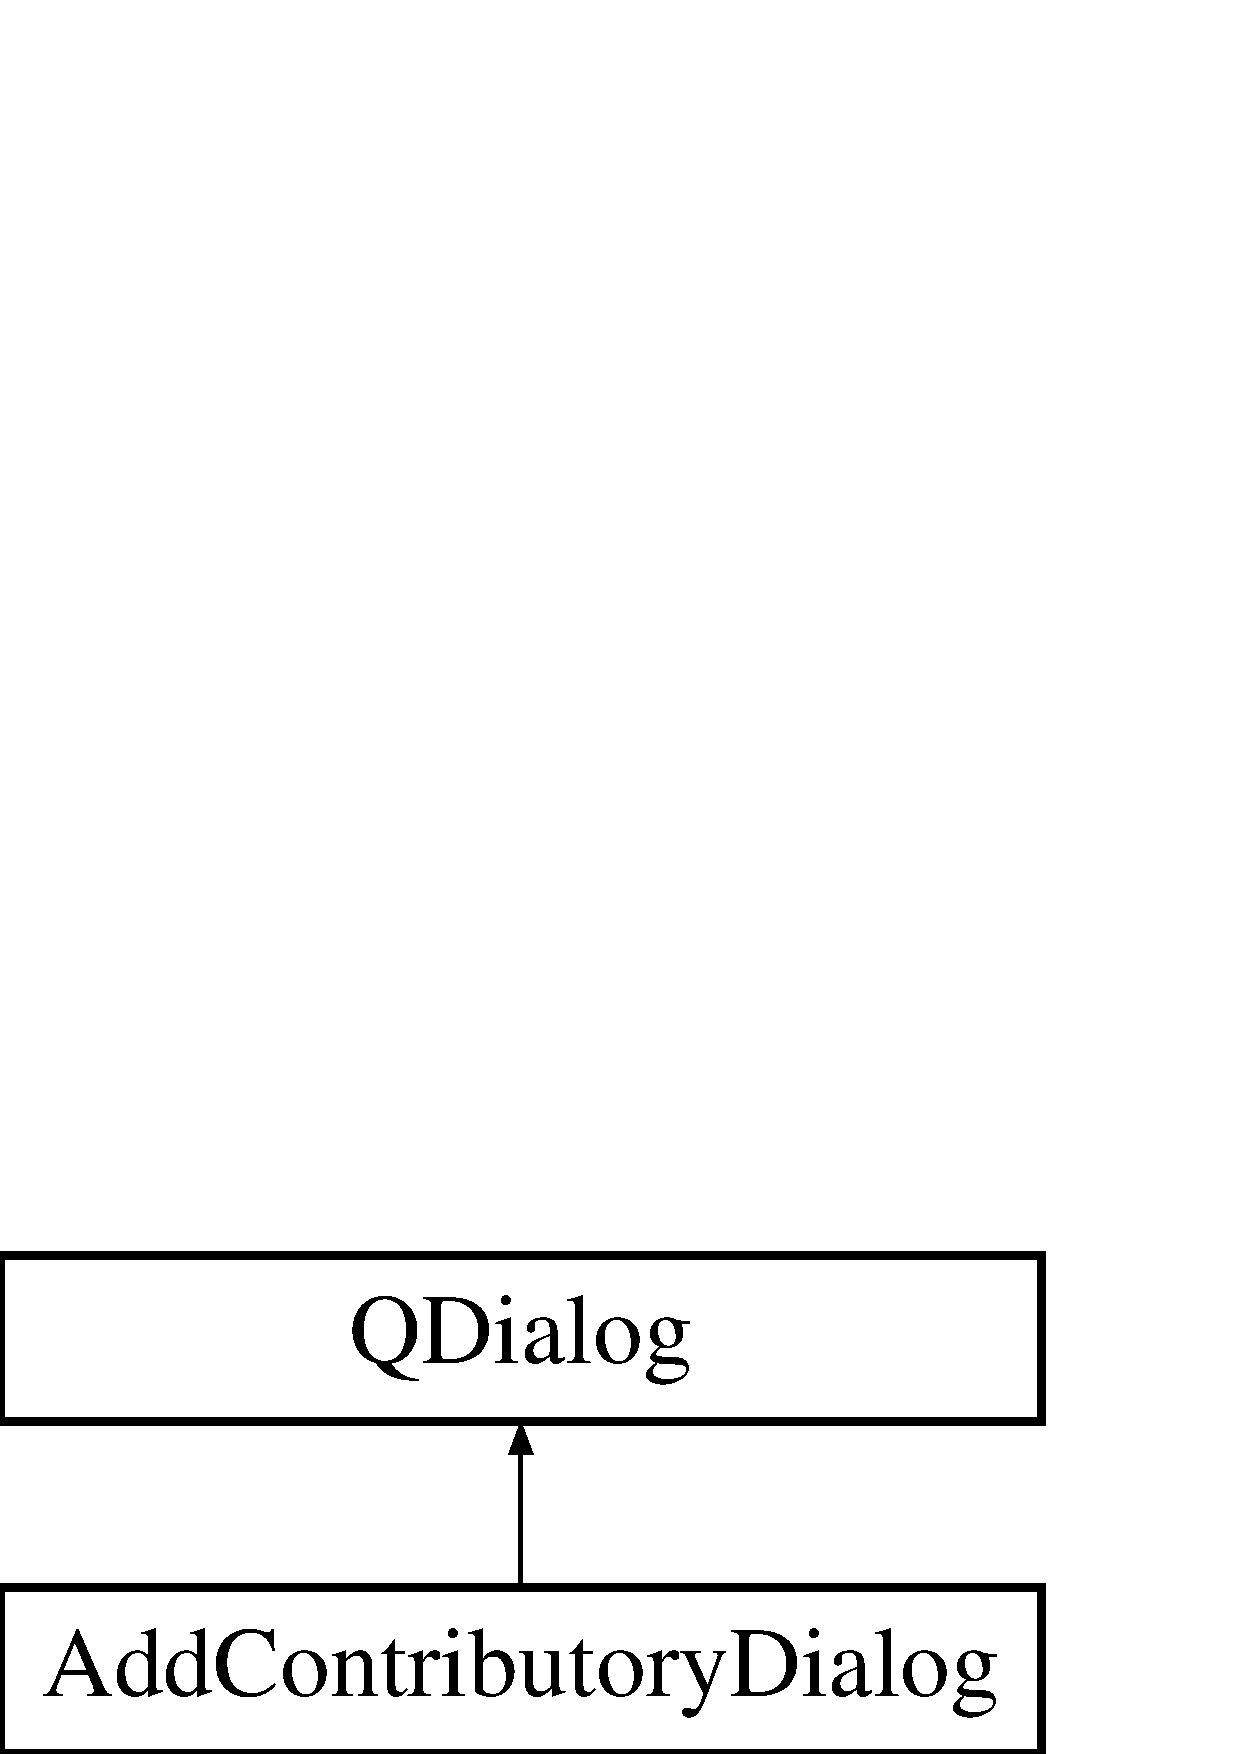
\includegraphics[height=2.000000cm]{d9/dfa/classAddContributoryDialog}
\end{center}
\end{figure}
\subsection*{Public Member Functions}
\begin{DoxyCompactItemize}
\item 
\hyperlink{classAddContributoryDialog_a75ef0d55afcf2cc30a702bb4792ccc2b}{Add\-Contributory\-Dialog} (Q\-Widget $\ast$parent=0)
\begin{DoxyCompactList}\small\item\em \hyperlink{classAddContributoryDialog}{Add\-Contributory\-Dialog} Construct a new windows Add\-Contributory. \end{DoxyCompactList}\end{DoxyCompactItemize}


\subsection{Detailed Description}
The \hyperlink{classAddContributoryDialog}{Add\-Contributory\-Dialog} class Windows to add a new \hyperlink{classContributory}{Contributory}. 

\begin{DoxyAuthor}{Author}
Florent Berbie 
\end{DoxyAuthor}


\subsection{Constructor \& Destructor Documentation}
\hypertarget{classAddContributoryDialog_a75ef0d55afcf2cc30a702bb4792ccc2b}{\index{Add\-Contributory\-Dialog@{Add\-Contributory\-Dialog}!Add\-Contributory\-Dialog@{Add\-Contributory\-Dialog}}
\index{Add\-Contributory\-Dialog@{Add\-Contributory\-Dialog}!AddContributoryDialog@{Add\-Contributory\-Dialog}}
\subsubsection[{Add\-Contributory\-Dialog}]{\setlength{\rightskip}{0pt plus 5cm}Add\-Contributory\-Dialog\-::\-Add\-Contributory\-Dialog (
\begin{DoxyParamCaption}
\item[{Q\-Widget $\ast$}]{parent = {\ttfamily 0}}
\end{DoxyParamCaption}
)\hspace{0.3cm}{\ttfamily [explicit]}}}\label{classAddContributoryDialog_a75ef0d55afcf2cc30a702bb4792ccc2b}


\hyperlink{classAddContributoryDialog}{Add\-Contributory\-Dialog} Construct a new windows Add\-Contributory. 


\begin{DoxyParams}{Parameters}
{\em parent} & Q\-Widget \\
\hline
\end{DoxyParams}


The documentation for this class was generated from the following files\-:\begin{DoxyCompactItemize}
\item 
/home/aroquemaurel/projets/qt/\-Fact\-Dev/src/dialogs/addcontributorydialog.\-h\item 
/home/aroquemaurel/projets/qt/\-Fact\-Dev/src/dialogs/addcontributorydialog.\-cpp\end{DoxyCompactItemize}

\hypertarget{classAddProjectDialog}{\section{Add\-Project\-Dialog Class Reference}
\label{classAddProjectDialog}\index{Add\-Project\-Dialog@{Add\-Project\-Dialog}}
}


The \hyperlink{classAddProjectDialog}{Add\-Project\-Dialog} class Windows to add a new \hyperlink{classProject}{Project}.  




{\ttfamily \#include $<$addprojectdialog.\-h$>$}

Inheritance diagram for Add\-Project\-Dialog\-:\begin{figure}[H]
\begin{center}
\leavevmode
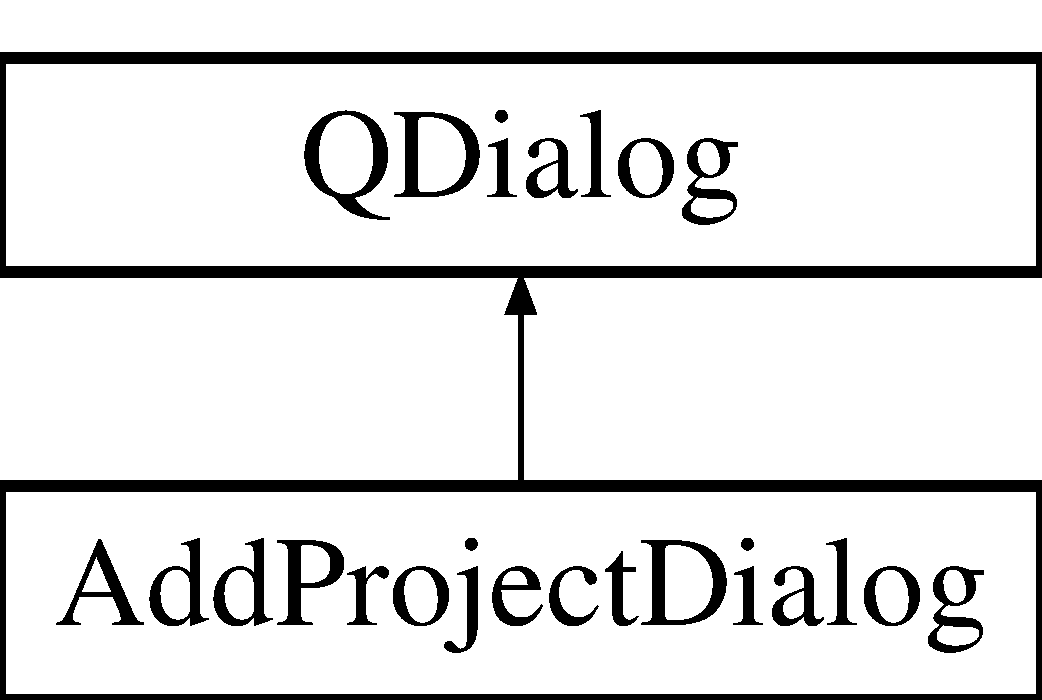
\includegraphics[height=2.000000cm]{d0/d23/classAddProjectDialog}
\end{center}
\end{figure}
\subsection*{Public Member Functions}
\begin{DoxyCompactItemize}
\item 
\hyperlink{classAddProjectDialog_abb96542ad074344f634d0ff834e65f03}{Add\-Project\-Dialog} (int id=0, Q\-Widget $\ast$parent=0)
\begin{DoxyCompactList}\small\item\em \hyperlink{classAddProjectDialog}{Add\-Project\-Dialog} Construct a windows \hyperlink{classAddProjectDialog}{Add\-Project\-Dialog}. \end{DoxyCompactList}\item 
\hypertarget{classAddProjectDialog_adb873176b67a671fc417e7ab21389c21}{void \hyperlink{classAddProjectDialog_adb873176b67a671fc417e7ab21389c21}{accept} ()}\label{classAddProjectDialog_adb873176b67a671fc417e7ab21389c21}

\begin{DoxyCompactList}\small\item\em accept Valid data inputed by user and add these data in \hyperlink{classDatabase}{Database} \end{DoxyCompactList}\item 
\hypertarget{classAddProjectDialog_a3e6011001312acd234f2352f1a796f0e}{void \hyperlink{classAddProjectDialog_a3e6011001312acd234f2352f1a796f0e}{reject} ()}\label{classAddProjectDialog_a3e6011001312acd234f2352f1a796f0e}

\begin{DoxyCompactList}\small\item\em reject Cancel the operation and close the windows \end{DoxyCompactList}\end{DoxyCompactItemize}


\subsection{Detailed Description}
The \hyperlink{classAddProjectDialog}{Add\-Project\-Dialog} class Windows to add a new \hyperlink{classProject}{Project}. 

\begin{DoxyAuthor}{Author}
Florent Berbie 
\end{DoxyAuthor}


\subsection{Constructor \& Destructor Documentation}
\hypertarget{classAddProjectDialog_abb96542ad074344f634d0ff834e65f03}{\index{Add\-Project\-Dialog@{Add\-Project\-Dialog}!Add\-Project\-Dialog@{Add\-Project\-Dialog}}
\index{Add\-Project\-Dialog@{Add\-Project\-Dialog}!AddProjectDialog@{Add\-Project\-Dialog}}
\subsubsection[{Add\-Project\-Dialog}]{\setlength{\rightskip}{0pt plus 5cm}Add\-Project\-Dialog\-::\-Add\-Project\-Dialog (
\begin{DoxyParamCaption}
\item[{int}]{id = {\ttfamily 0}, }
\item[{Q\-Widget $\ast$}]{parent = {\ttfamily 0}}
\end{DoxyParamCaption}
)\hspace{0.3cm}{\ttfamily [explicit]}}}\label{classAddProjectDialog_abb96542ad074344f634d0ff834e65f03}


\hyperlink{classAddProjectDialog}{Add\-Project\-Dialog} Construct a windows \hyperlink{classAddProjectDialog}{Add\-Project\-Dialog}. 


\begin{DoxyParams}{Parameters}
{\em id} & \hyperlink{classProject}{Project} identity \\
\hline
{\em parent} & Q\-Widget of the current windows \\
\hline
\end{DoxyParams}


The documentation for this class was generated from the following files\-:\begin{DoxyCompactItemize}
\item 
/home/florent/\-Documents/\-Projet\-\_\-\-S8/\-Fact\-Dev/src/dialogs/addprojectdialog.\-h\item 
/home/florent/\-Documents/\-Projet\-\_\-\-S8/\-Fact\-Dev/src/dialogs/addprojectdialog.\-cpp\end{DoxyCompactItemize}

\hypertarget{classBilling}{\section{Billing Class Reference}
\label{classBilling}\index{Billing@{Billing}}
}


The \hyperlink{classBilling}{Billing} class \-: \hyperlink{classBilling}{Billing} of a \hyperlink{classCustomer}{Customer}.  




{\ttfamily \#include $<$billing.\-h$>$}

Inheritance diagram for Billing\-:\begin{figure}[H]
\begin{center}
\leavevmode
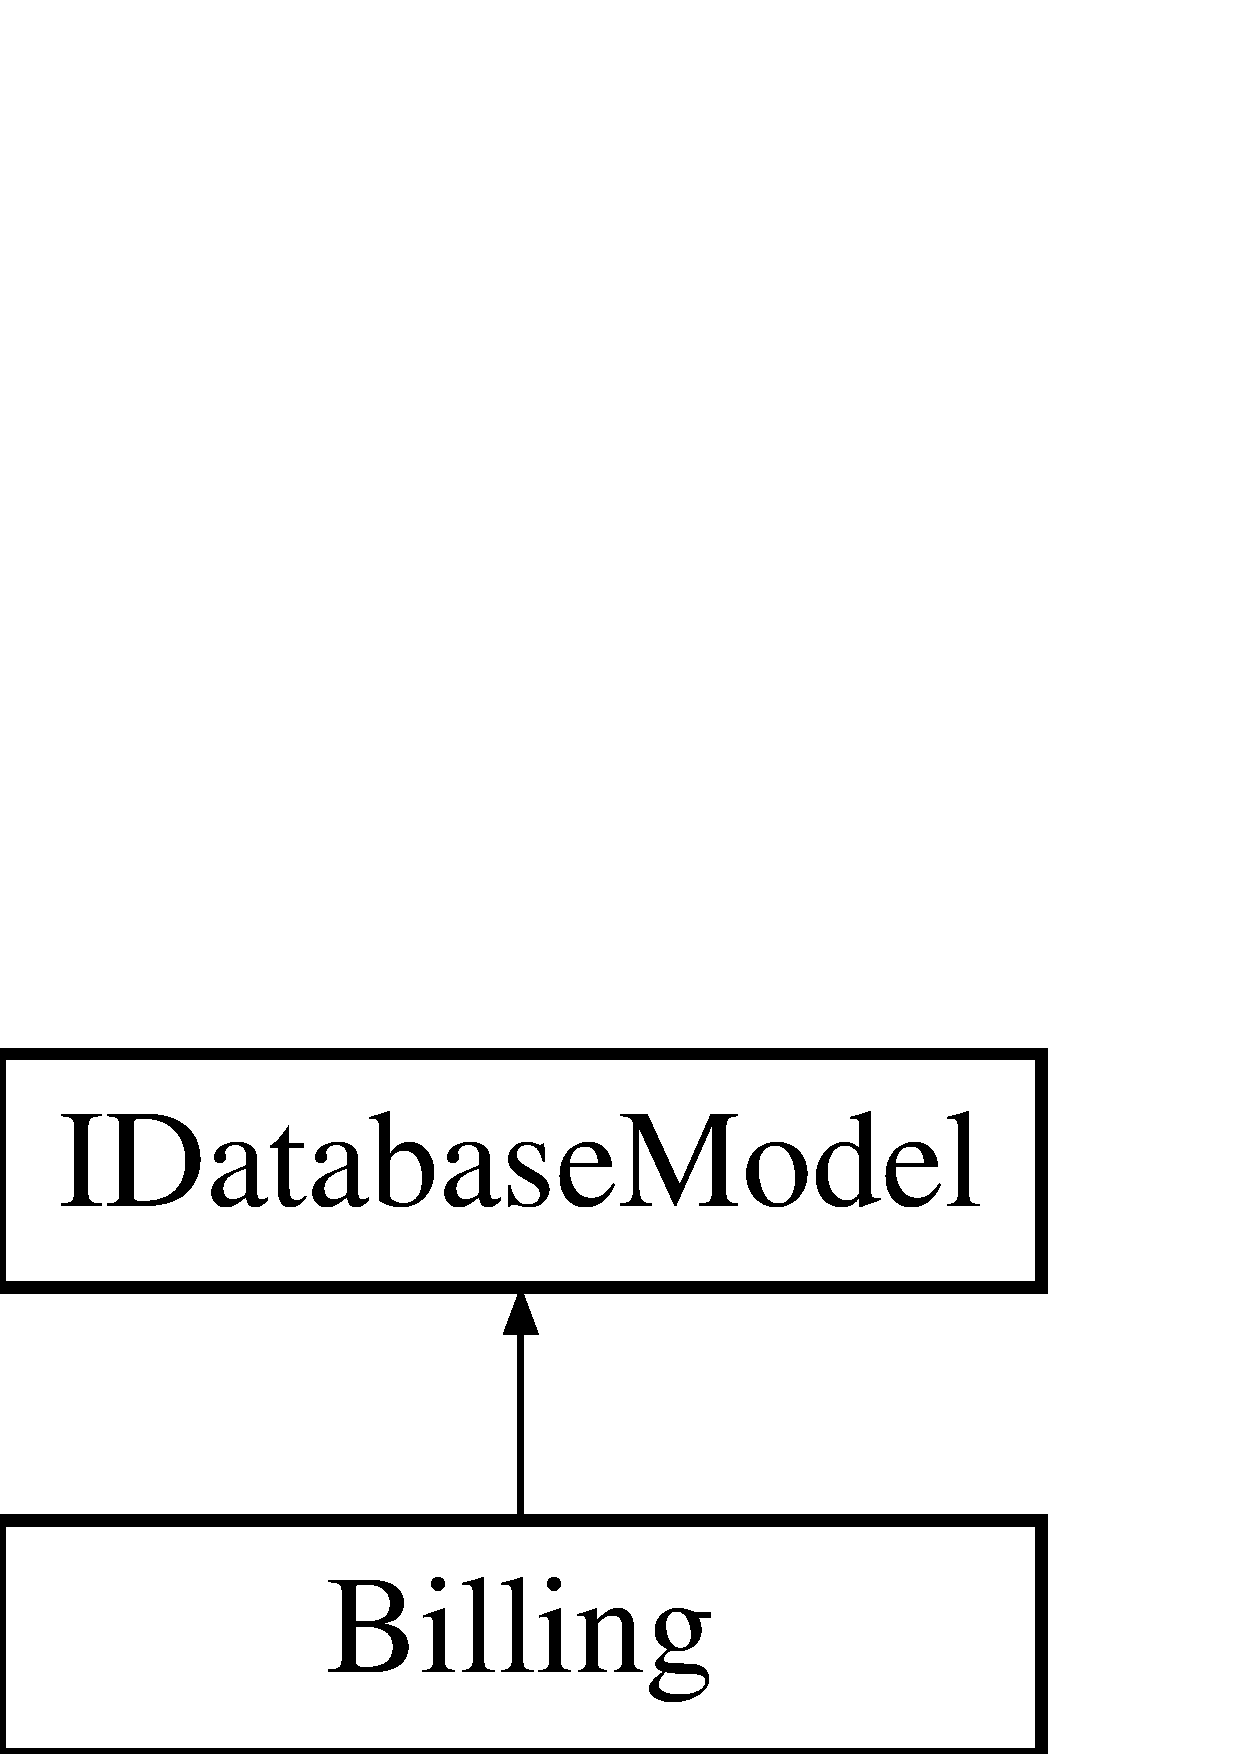
\includegraphics[height=2.000000cm]{df/d81/classBilling}
\end{center}
\end{figure}
\subsection*{Public Member Functions}
\begin{DoxyCompactItemize}
\item 
\hypertarget{classBilling_a8e7a38f9ef550c20ce1bf6b46153defa}{\hyperlink{classBilling_a8e7a38f9ef550c20ce1bf6b46153defa}{Billing} ()}\label{classBilling_a8e7a38f9ef550c20ce1bf6b46153defa}

\begin{DoxyCompactList}\small\item\em \hyperlink{classBilling_a8e7a38f9ef550c20ce1bf6b46153defa}{Billing\-::\-Billing}. Construct a \hyperlink{classBilling}{Billing}. \end{DoxyCompactList}\item 
\hypertarget{classBilling_a3d96a6baed6ca2d2e1096496f0fd3270}{void \hyperlink{classBilling_a3d96a6baed6ca2d2e1096496f0fd3270}{commit} ()}\label{classBilling_a3d96a6baed6ca2d2e1096496f0fd3270}

\begin{DoxyCompactList}\small\item\em \hyperlink{classBilling_a3d96a6baed6ca2d2e1096496f0fd3270}{Billing\-::commit}. Insert a modification in \hyperlink{classBilling}{Billing} table on the database. \end{DoxyCompactList}\item 
void \hyperlink{classBilling_a8beb72061cd53a964cf0ba3f04686613}{hydrat} (int get\-Id)
\begin{DoxyCompactList}\small\item\em \hyperlink{classBilling_a8beb72061cd53a964cf0ba3f04686613}{Billing\-::hydrat}. Update of the \hyperlink{classBilling}{Billing} which is specified by {\itshape get\-Id} \end{DoxyCompactList}\item 
\hypertarget{classBilling_ab5efe0286d292707073b9f1cecd98d6f}{void \hyperlink{classBilling_ab5efe0286d292707073b9f1cecd98d6f}{remove} ()}\label{classBilling_ab5efe0286d292707073b9f1cecd98d6f}

\begin{DoxyCompactList}\small\item\em \hyperlink{classBilling_ab5efe0286d292707073b9f1cecd98d6f}{Billing\-::remove}. Remove a \hyperlink{classBilling}{Billing}. \end{DoxyCompactList}\item 
Q\-Map$<$ \hyperlink{classProject}{Project}, Q\-List\\*
$<$ \hyperlink{classContributory}{Contributory} $>$ $>$ \hyperlink{classBilling_a08416c71eee43ec294e666ce45d43856}{get\-Contributories} () const 
\begin{DoxyCompactList}\small\item\em \hyperlink{classBilling_a08416c71eee43ec294e666ce45d43856}{Billing\-::get\-Contributories}. Return a map of {\bfseries \hyperlink{classContributory}{Contributory}} for each {\bfseries \hyperlink{classProject}{Project}} of the {\bfseries \hyperlink{classBilling}{Billing}} \end{DoxyCompactList}\item 
\hypertarget{classBilling_a25706aa084df2f345aaa1323130f78b4}{void {\bfseries set\-Contributories} (const Q\-Map$<$ \hyperlink{classProject}{Project}, Q\-List$<$ \hyperlink{classContributory}{Contributory} $>$ $>$ \&\hyperlink{classBilling_a08416c71eee43ec294e666ce45d43856}{get\-Contributories})}\label{classBilling_a25706aa084df2f345aaa1323130f78b4}

\item 
Q\-String \hyperlink{classBilling_ad817d4a1dfa011d20b4358a896662f0e}{get\-Title} () const 
\begin{DoxyCompactList}\small\item\em \hyperlink{classBilling_ad817d4a1dfa011d20b4358a896662f0e}{Billing\-::get\-Title}. return title of {\bfseries \hyperlink{classBilling}{Billing}} \end{DoxyCompactList}\item 
void \hyperlink{classBilling_a3e5e98325bd0e9fb4c253ddf07bf66c8}{set\-Title} (const Q\-String \&\hyperlink{classBilling_ad817d4a1dfa011d20b4358a896662f0e}{get\-Title})
\begin{DoxyCompactList}\small\item\em \hyperlink{classBilling_a3e5e98325bd0e9fb4c253ddf07bf66c8}{Billing\-::set\-Title}. Modify the title of {\bfseries \hyperlink{classBilling}{Billing}} \end{DoxyCompactList}\item 
int \hyperlink{classBilling_a23a9446aef6af58bcfa698b76cc24731}{get\-Number} () const 
\begin{DoxyCompactList}\small\item\em \hyperlink{classBilling_a23a9446aef6af58bcfa698b76cc24731}{Billing\-::get\-Number}. Return number of the {\bfseries \hyperlink{classBilling}{Billing}}. \end{DoxyCompactList}\item 
void \hyperlink{classBilling_a1178eab66407b0761c35a13d8da84cdb}{set\-Number} (int \hyperlink{classBilling_a23a9446aef6af58bcfa698b76cc24731}{get\-Number})
\begin{DoxyCompactList}\small\item\em \hyperlink{classBilling_a1178eab66407b0761c35a13d8da84cdb}{Billing\-::set\-Number}. Modify {\itshape \-\_\-number} of \hyperlink{classBilling}{Billing}. \end{DoxyCompactList}\item 
bool \hyperlink{classBilling_ad616bbb5664e0ba2bac6982f06a7c723}{is\-Billing} () const 
\begin{DoxyCompactList}\small\item\em \hyperlink{classBilling_ad616bbb5664e0ba2bac6982f06a7c723}{Billing\-::is\-Billing}. Return if it's a billing or a quote. \end{DoxyCompactList}\item 
void \hyperlink{classBilling_a81a3b85e0e051239521b4e3d93f297c2}{set\-Is\-Billing} (bool \hyperlink{classBilling_ad616bbb5664e0ba2bac6982f06a7c723}{is\-Billing})
\begin{DoxyCompactList}\small\item\em \hyperlink{classBilling_a81a3b85e0e051239521b4e3d93f297c2}{Billing\-::set\-Is\-Billing}. Modify {\itshape is\-Billing} of {\bfseries \hyperlink{classBilling}{Billing}}. \end{DoxyCompactList}\item 
Q\-Date \hyperlink{classBilling_ad3657e1cdf05613cfca4b22b62976213}{get\-Date} () const 
\begin{DoxyCompactList}\small\item\em \hyperlink{classBilling_ad3657e1cdf05613cfca4b22b62976213}{Billing\-::get\-Date}. return date of the {\bfseries \hyperlink{classBilling}{Billing}} \end{DoxyCompactList}\item 
void \hyperlink{classBilling_ad1cb89772dc12335543ff7d422d18bd4}{set\-Date} (const Q\-Date \&\hyperlink{classBilling_ad3657e1cdf05613cfca4b22b62976213}{get\-Date})
\begin{DoxyCompactList}\small\item\em \hyperlink{classBilling_ad1cb89772dc12335543ff7d422d18bd4}{Billing\-::set\-Date}. Modify {\itshape date} of the {\bfseries \hyperlink{classBilling}{Billing}} \end{DoxyCompactList}\end{DoxyCompactItemize}
\subsection*{Additional Inherited Members}


\subsection{Detailed Description}
The \hyperlink{classBilling}{Billing} class \-: \hyperlink{classBilling}{Billing} of a \hyperlink{classCustomer}{Customer}. 

\subsection{Member Function Documentation}
\hypertarget{classBilling_a08416c71eee43ec294e666ce45d43856}{\index{Billing@{Billing}!get\-Contributories@{get\-Contributories}}
\index{get\-Contributories@{get\-Contributories}!Billing@{Billing}}
\subsubsection[{get\-Contributories}]{\setlength{\rightskip}{0pt plus 5cm}Q\-Map$<$ {\bf Project}, Q\-List$<$ {\bf Contributory} $>$ $>$ Billing\-::get\-Contributories (
\begin{DoxyParamCaption}
{}
\end{DoxyParamCaption}
) const}}\label{classBilling_a08416c71eee43ec294e666ce45d43856}


\hyperlink{classBilling_a08416c71eee43ec294e666ce45d43856}{Billing\-::get\-Contributories}. Return a map of {\bfseries \hyperlink{classContributory}{Contributory}} for each {\bfseries \hyperlink{classProject}{Project}} of the {\bfseries \hyperlink{classBilling}{Billing}} 

\begin{DoxyReturn}{Returns}
Q\-Map$<$\hyperlink{classProject}{Project}, Q\-List$<$\-Contributory$>$$>$ 
\end{DoxyReturn}
\hypertarget{classBilling_ad3657e1cdf05613cfca4b22b62976213}{\index{Billing@{Billing}!get\-Date@{get\-Date}}
\index{get\-Date@{get\-Date}!Billing@{Billing}}
\subsubsection[{get\-Date}]{\setlength{\rightskip}{0pt plus 5cm}Q\-Date Billing\-::get\-Date (
\begin{DoxyParamCaption}
{}
\end{DoxyParamCaption}
) const}}\label{classBilling_ad3657e1cdf05613cfca4b22b62976213}


\hyperlink{classBilling_ad3657e1cdf05613cfca4b22b62976213}{Billing\-::get\-Date}. return date of the {\bfseries \hyperlink{classBilling}{Billing}} 

\begin{DoxyReturn}{Returns}
date of \hyperlink{classBilling}{Billing} 
\end{DoxyReturn}
\hypertarget{classBilling_a23a9446aef6af58bcfa698b76cc24731}{\index{Billing@{Billing}!get\-Number@{get\-Number}}
\index{get\-Number@{get\-Number}!Billing@{Billing}}
\subsubsection[{get\-Number}]{\setlength{\rightskip}{0pt plus 5cm}int Billing\-::get\-Number (
\begin{DoxyParamCaption}
{}
\end{DoxyParamCaption}
) const}}\label{classBilling_a23a9446aef6af58bcfa698b76cc24731}


\hyperlink{classBilling_a23a9446aef6af58bcfa698b76cc24731}{Billing\-::get\-Number}. Return number of the {\bfseries \hyperlink{classBilling}{Billing}}. 

\begin{DoxyReturn}{Returns}
\-\_\-number of \hyperlink{classBilling}{Billing} 
\end{DoxyReturn}
\hypertarget{classBilling_ad817d4a1dfa011d20b4358a896662f0e}{\index{Billing@{Billing}!get\-Title@{get\-Title}}
\index{get\-Title@{get\-Title}!Billing@{Billing}}
\subsubsection[{get\-Title}]{\setlength{\rightskip}{0pt plus 5cm}Q\-String Billing\-::get\-Title (
\begin{DoxyParamCaption}
{}
\end{DoxyParamCaption}
) const}}\label{classBilling_ad817d4a1dfa011d20b4358a896662f0e}


\hyperlink{classBilling_ad817d4a1dfa011d20b4358a896662f0e}{Billing\-::get\-Title}. return title of {\bfseries \hyperlink{classBilling}{Billing}} 

\begin{DoxyReturn}{Returns}
title of \hyperlink{classBilling}{Billing} 
\end{DoxyReturn}
\hypertarget{classBilling_a8beb72061cd53a964cf0ba3f04686613}{\index{Billing@{Billing}!hydrat@{hydrat}}
\index{hydrat@{hydrat}!Billing@{Billing}}
\subsubsection[{hydrat}]{\setlength{\rightskip}{0pt plus 5cm}void Billing\-::hydrat (
\begin{DoxyParamCaption}
\item[{int}]{get\-Id}
\end{DoxyParamCaption}
)\hspace{0.3cm}{\ttfamily [virtual]}}}\label{classBilling_a8beb72061cd53a964cf0ba3f04686613}


\hyperlink{classBilling_a8beb72061cd53a964cf0ba3f04686613}{Billing\-::hydrat}. Update of the \hyperlink{classBilling}{Billing} which is specified by {\itshape get\-Id} 


\begin{DoxyParams}{Parameters}
{\em get\-Id} & \\
\hline
\end{DoxyParams}


Implements \hyperlink{classIDatabaseModel}{I\-Database\-Model}.

\hypertarget{classBilling_ad616bbb5664e0ba2bac6982f06a7c723}{\index{Billing@{Billing}!is\-Billing@{is\-Billing}}
\index{is\-Billing@{is\-Billing}!Billing@{Billing}}
\subsubsection[{is\-Billing}]{\setlength{\rightskip}{0pt plus 5cm}bool Billing\-::is\-Billing (
\begin{DoxyParamCaption}
{}
\end{DoxyParamCaption}
) const}}\label{classBilling_ad616bbb5664e0ba2bac6982f06a7c723}


\hyperlink{classBilling_ad616bbb5664e0ba2bac6982f06a7c723}{Billing\-::is\-Billing}. Return if it's a billing or a quote. 

\begin{DoxyReturn}{Returns}
if it's billing or a quote 
\end{DoxyReturn}
\hypertarget{classBilling_ad1cb89772dc12335543ff7d422d18bd4}{\index{Billing@{Billing}!set\-Date@{set\-Date}}
\index{set\-Date@{set\-Date}!Billing@{Billing}}
\subsubsection[{set\-Date}]{\setlength{\rightskip}{0pt plus 5cm}void Billing\-::set\-Date (
\begin{DoxyParamCaption}
\item[{const Q\-Date \&}]{get\-Date}
\end{DoxyParamCaption}
)}}\label{classBilling_ad1cb89772dc12335543ff7d422d18bd4}


\hyperlink{classBilling_ad1cb89772dc12335543ff7d422d18bd4}{Billing\-::set\-Date}. Modify {\itshape date} of the {\bfseries \hyperlink{classBilling}{Billing}} 


\begin{DoxyParams}{Parameters}
{\em get\-Date} & the new date of the \hyperlink{classBilling}{Billing} \\
\hline
\end{DoxyParams}
\hypertarget{classBilling_a81a3b85e0e051239521b4e3d93f297c2}{\index{Billing@{Billing}!set\-Is\-Billing@{set\-Is\-Billing}}
\index{set\-Is\-Billing@{set\-Is\-Billing}!Billing@{Billing}}
\subsubsection[{set\-Is\-Billing}]{\setlength{\rightskip}{0pt plus 5cm}void Billing\-::set\-Is\-Billing (
\begin{DoxyParamCaption}
\item[{bool}]{is\-Billing}
\end{DoxyParamCaption}
)}}\label{classBilling_a81a3b85e0e051239521b4e3d93f297c2}


\hyperlink{classBilling_a81a3b85e0e051239521b4e3d93f297c2}{Billing\-::set\-Is\-Billing}. Modify {\itshape is\-Billing} of {\bfseries \hyperlink{classBilling}{Billing}}. 


\begin{DoxyParams}{Parameters}
{\em is\-Billing} & \\
\hline
\end{DoxyParams}
\hypertarget{classBilling_a1178eab66407b0761c35a13d8da84cdb}{\index{Billing@{Billing}!set\-Number@{set\-Number}}
\index{set\-Number@{set\-Number}!Billing@{Billing}}
\subsubsection[{set\-Number}]{\setlength{\rightskip}{0pt plus 5cm}void Billing\-::set\-Number (
\begin{DoxyParamCaption}
\item[{int}]{get\-Number}
\end{DoxyParamCaption}
)}}\label{classBilling_a1178eab66407b0761c35a13d8da84cdb}


\hyperlink{classBilling_a1178eab66407b0761c35a13d8da84cdb}{Billing\-::set\-Number}. Modify {\itshape \-\_\-number} of \hyperlink{classBilling}{Billing}. 


\begin{DoxyParams}{Parameters}
{\em get\-Number} & the new number of the \hyperlink{classBilling}{Billing} \\
\hline
\end{DoxyParams}
\hypertarget{classBilling_a3e5e98325bd0e9fb4c253ddf07bf66c8}{\index{Billing@{Billing}!set\-Title@{set\-Title}}
\index{set\-Title@{set\-Title}!Billing@{Billing}}
\subsubsection[{set\-Title}]{\setlength{\rightskip}{0pt plus 5cm}void Billing\-::set\-Title (
\begin{DoxyParamCaption}
\item[{const Q\-String \&}]{get\-Title}
\end{DoxyParamCaption}
)}}\label{classBilling_a3e5e98325bd0e9fb4c253ddf07bf66c8}


\hyperlink{classBilling_a3e5e98325bd0e9fb4c253ddf07bf66c8}{Billing\-::set\-Title}. Modify the title of {\bfseries \hyperlink{classBilling}{Billing}} 


\begin{DoxyParams}{Parameters}
{\em get\-Title} & Modify the title with {\itshape get\-Title} \\
\hline
\end{DoxyParams}


The documentation for this class was generated from the following files\-:\begin{DoxyCompactItemize}
\item 
/home/florent/\-Documents/\-Projet\-\_\-\-S8/\-Fact\-Dev/src/models/billing.\-h\item 
/home/florent/\-Documents/\-Projet\-\_\-\-S8/\-Fact\-Dev/src/models/billing.\-cpp\end{DoxyCompactItemize}

\hypertarget{classComboBoxModelWidget}{\section{Combo\+Box\+Model\+Widget Class Reference}
\label{classComboBoxModelWidget}\index{Combo\+Box\+Model\+Widget@{Combo\+Box\+Model\+Widget}}
}


The \hyperlink{classComboBoxModelWidget}{Combo\+Box\+Model\+Widget} class T\+O\+D\+O.  




{\ttfamily \#include $<$comboboxmodelwidget.\+h$>$}

Inheritance diagram for Combo\+Box\+Model\+Widget\+:\begin{figure}[H]
\begin{center}
\leavevmode
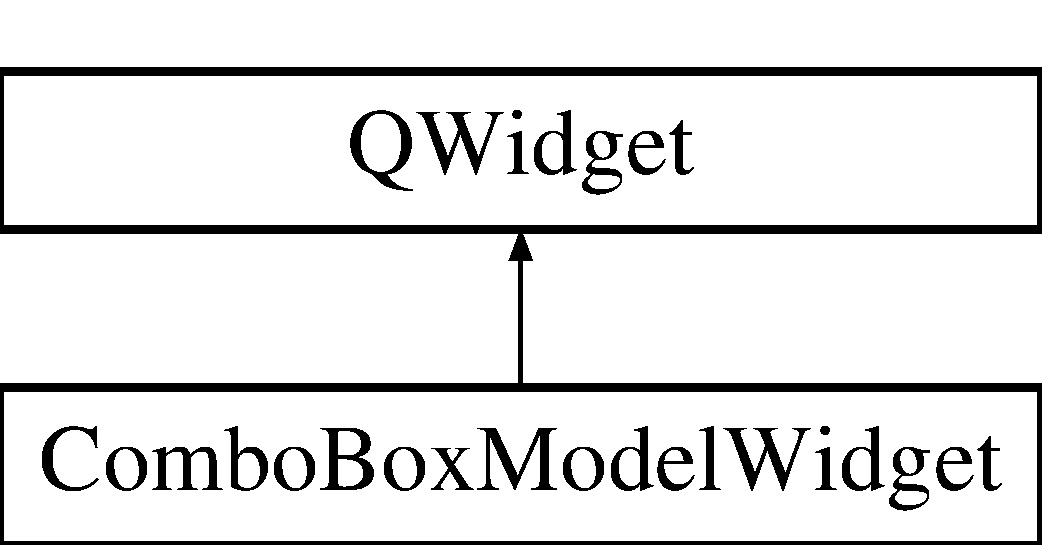
\includegraphics[height=2.000000cm]{d5/d79/classComboBoxModelWidget}
\end{center}
\end{figure}
\subsection*{Public Member Functions}
\begin{DoxyCompactItemize}
\item 
\hypertarget{classComboBoxModelWidget_a8632edda11e66ee50cfc89729b2feb3a}{{\bfseries Combo\+Box\+Model\+Widget} (Q\+Widget $\ast$parent=0)}\label{classComboBoxModelWidget_a8632edda11e66ee50cfc89729b2feb3a}

\end{DoxyCompactItemize}


\subsection{Detailed Description}
The \hyperlink{classComboBoxModelWidget}{Combo\+Box\+Model\+Widget} class T\+O\+D\+O. 

The documentation for this class was generated from the following files\+:\begin{DoxyCompactItemize}
\item 
src/widgets/comboboxmodelwidget.\+h\item 
src/widgets/comboboxmodelwidget.\+cpp\end{DoxyCompactItemize}

\hypertarget{classContributory}{\section{Contributory Class Reference}
\label{classContributory}\index{Contributory@{Contributory}}
}


The \hyperlink{classContributory}{Contributory} class.  




{\ttfamily \#include $<$contributory.\+h$>$}

Inheritance diagram for Contributory\+:\begin{figure}[H]
\begin{center}
\leavevmode
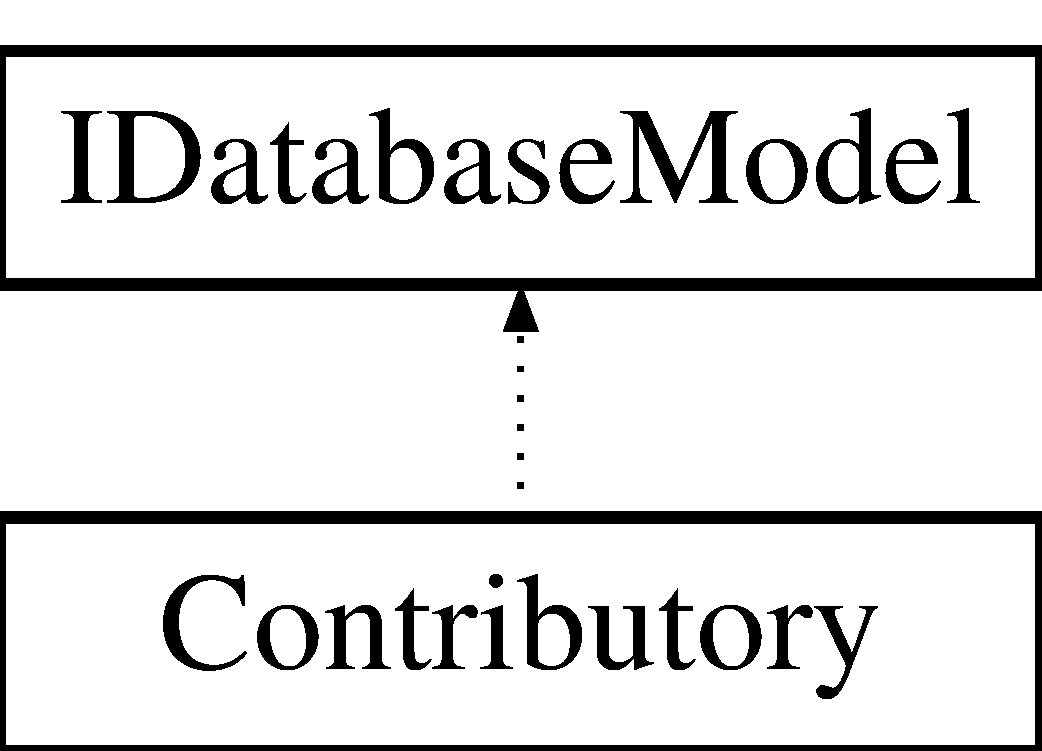
\includegraphics[height=2.000000cm]{d5/d09/classContributory}
\end{center}
\end{figure}
\subsection*{Public Member Functions}
\begin{DoxyCompactItemize}
\item 
\hypertarget{classContributory_a5991c01efd2dedcbbddde252c48d7af8}{\hyperlink{classContributory_a5991c01efd2dedcbbddde252c48d7af8}{Contributory} ()}\label{classContributory_a5991c01efd2dedcbbddde252c48d7af8}

\begin{DoxyCompactList}\small\item\em \hyperlink{classContributory_a5991c01efd2dedcbbddde252c48d7af8}{Contributory\+::\+Contributory} Contruct a \hyperlink{classContributory}{Contributory}. \end{DoxyCompactList}\item 
\hyperlink{classContributory_a5c72cf02d2c6d25ee736af711edd76ec}{Contributory} (int id)
\begin{DoxyCompactList}\small\item\em \hyperlink{classContributory_a5991c01efd2dedcbbddde252c48d7af8}{Contributory\+::\+Contributory} Contruct a \hyperlink{classContributory}{Contributory} and get data in database. \end{DoxyCompactList}\item 
\hypertarget{classContributory_a5c09902237bba780b594129dc2fa60d6}{void \hyperlink{classContributory_a5c09902237bba780b594129dc2fa60d6}{commit} ()}\label{classContributory_a5c09902237bba780b594129dc2fa60d6}

\begin{DoxyCompactList}\small\item\em \hyperlink{classContributory_a5c09902237bba780b594129dc2fa60d6}{Contributory\+::commit} Update or insert a contributory to the database. \end{DoxyCompactList}\item 
void \hyperlink{classContributory_a2b834e0288c93ba9ed70acf7a0b8c32d}{hydrat} (int id)
\begin{DoxyCompactList}\small\item\em \hyperlink{classContributory_a2b834e0288c93ba9ed70acf7a0b8c32d}{Contributory\+::hydrat} Get data about the \hyperlink{classContributory}{Contributory} which is specified by the identify {\itshape id} \end{DoxyCompactList}\item 
\hypertarget{classContributory_a59641dbc35947c31eb841b46fed6130f}{void \hyperlink{classContributory_a59641dbc35947c31eb841b46fed6130f}{remove} ()}\label{classContributory_a59641dbc35947c31eb841b46fed6130f}

\begin{DoxyCompactList}\small\item\em \hyperlink{classContributory_a59641dbc35947c31eb841b46fed6130f}{Contributory\+::remove} Remove the current \hyperlink{classContributory}{Contributory}. \end{DoxyCompactList}\item 
\hyperlink{classProject}{Project} $\ast$ \hyperlink{classContributory_ab36c08e9844bc327e196a472733ac417}{get\+Project} () const 
\begin{DoxyCompactList}\small\item\em \hyperlink{classContributory_ab36c08e9844bc327e196a472733ac417}{Contributory\+::get\+Project} Return the project linked to this \hyperlink{classContributory}{Contributory}. \end{DoxyCompactList}\item 
void \hyperlink{classContributory_a72088580dc62d1d7a1a7674f8ab9a492}{set\+Project} (\hyperlink{classProject}{Project} $\ast$id)
\begin{DoxyCompactList}\small\item\em \hyperlink{classContributory_a72088580dc62d1d7a1a7674f8ab9a492}{Contributory\+::set\+Project} Modify the identify {\itshape id} of the \hyperlink{classProject}{Project} linke to this \hyperlink{classContributory}{Contributory}. \end{DoxyCompactList}\item 
double \hyperlink{classContributory_a01eccd2a6cea09c295bd808a08d27efe}{get\+Nb\+Hours} () const 
\begin{DoxyCompactList}\small\item\em get\+Nb\+Hours Number of work hour of a contributory \end{DoxyCompactList}\item 
void \hyperlink{classContributory_a32d589c7cb5269aad6c70ad6703c4d58}{set\+Nb\+Hours} (double value)
\begin{DoxyCompactList}\small\item\em set\+Nb\+Hours Change nb\+Hours \end{DoxyCompactList}\item 
Q\+String \hyperlink{classContributory_ae960d1562ede18bbddd2d8bccea762b7}{get\+Description} () const 
\begin{DoxyCompactList}\small\item\em get\+Description Description of a contributory \end{DoxyCompactList}\item 
void \hyperlink{classContributory_a76af91dd9dfb28cc59fcc9685db8d3e5}{set\+Description} (const Q\+String \&\hyperlink{classContributory_ae960d1562ede18bbddd2d8bccea762b7}{get\+Description})
\begin{DoxyCompactList}\small\item\em set\+Description Change the contributory description \end{DoxyCompactList}\end{DoxyCompactItemize}
\subsection*{Additional Inherited Members}


\subsection{Detailed Description}
The \hyperlink{classContributory}{Contributory} class. 

\begin{DoxyAuthor}{Author}

\end{DoxyAuthor}


\subsection{Constructor \& Destructor Documentation}
\hypertarget{classContributory_a5c72cf02d2c6d25ee736af711edd76ec}{\index{Contributory@{Contributory}!Contributory@{Contributory}}
\index{Contributory@{Contributory}!Contributory@{Contributory}}
\subsubsection[{Contributory}]{\setlength{\rightskip}{0pt plus 5cm}Contributory\+::\+Contributory (
\begin{DoxyParamCaption}
\item[{int}]{id}
\end{DoxyParamCaption}
)}}\label{classContributory_a5c72cf02d2c6d25ee736af711edd76ec}


\hyperlink{classContributory_a5991c01efd2dedcbbddde252c48d7af8}{Contributory\+::\+Contributory} Contruct a \hyperlink{classContributory}{Contributory} and get data in database. 


\begin{DoxyParams}{Parameters}
{\em id} & \hyperlink{classContributory}{Contributory}'s id \\
\hline
\end{DoxyParams}


\subsection{Member Function Documentation}
\hypertarget{classContributory_ae960d1562ede18bbddd2d8bccea762b7}{\index{Contributory@{Contributory}!get\+Description@{get\+Description}}
\index{get\+Description@{get\+Description}!Contributory@{Contributory}}
\subsubsection[{get\+Description}]{\setlength{\rightskip}{0pt plus 5cm}Q\+String Contributory\+::get\+Description (
\begin{DoxyParamCaption}
{}
\end{DoxyParamCaption}
) const}}\label{classContributory_ae960d1562ede18bbddd2d8bccea762b7}


get\+Description Description of a contributory 

\begin{DoxyReturn}{Returns}
The description 
\end{DoxyReturn}
\hypertarget{classContributory_a01eccd2a6cea09c295bd808a08d27efe}{\index{Contributory@{Contributory}!get\+Nb\+Hours@{get\+Nb\+Hours}}
\index{get\+Nb\+Hours@{get\+Nb\+Hours}!Contributory@{Contributory}}
\subsubsection[{get\+Nb\+Hours}]{\setlength{\rightskip}{0pt plus 5cm}double Contributory\+::get\+Nb\+Hours (
\begin{DoxyParamCaption}
{}
\end{DoxyParamCaption}
) const}}\label{classContributory_a01eccd2a6cea09c295bd808a08d27efe}


get\+Nb\+Hours Number of work hour of a contributory 

\begin{DoxyReturn}{Returns}
Then number of hours 
\end{DoxyReturn}
\hypertarget{classContributory_ab36c08e9844bc327e196a472733ac417}{\index{Contributory@{Contributory}!get\+Project@{get\+Project}}
\index{get\+Project@{get\+Project}!Contributory@{Contributory}}
\subsubsection[{get\+Project}]{\setlength{\rightskip}{0pt plus 5cm}{\bf Project} $\ast$ Contributory\+::get\+Project (
\begin{DoxyParamCaption}
{}
\end{DoxyParamCaption}
) const}}\label{classContributory_ab36c08e9844bc327e196a472733ac417}


\hyperlink{classContributory_ab36c08e9844bc327e196a472733ac417}{Contributory\+::get\+Project} Return the project linked to this \hyperlink{classContributory}{Contributory}. 

\begin{DoxyReturn}{Returns}
\hyperlink{classProject}{Project} linked to this \hyperlink{classContributory}{Contributory} 
\end{DoxyReturn}
\hypertarget{classContributory_a2b834e0288c93ba9ed70acf7a0b8c32d}{\index{Contributory@{Contributory}!hydrat@{hydrat}}
\index{hydrat@{hydrat}!Contributory@{Contributory}}
\subsubsection[{hydrat}]{\setlength{\rightskip}{0pt plus 5cm}void Contributory\+::hydrat (
\begin{DoxyParamCaption}
\item[{int}]{id}
\end{DoxyParamCaption}
)\hspace{0.3cm}{\ttfamily [virtual]}}}\label{classContributory_a2b834e0288c93ba9ed70acf7a0b8c32d}


\hyperlink{classContributory_a2b834e0288c93ba9ed70acf7a0b8c32d}{Contributory\+::hydrat} Get data about the \hyperlink{classContributory}{Contributory} which is specified by the identify {\itshape id} 


\begin{DoxyParams}{Parameters}
{\em id} & \hyperlink{classContributory}{Contributory} identify \\
\hline
\end{DoxyParams}


Implements \hyperlink{classIDatabaseModel_a25e44ed10a75976f86e14d34aea02c37}{I\+Database\+Model}.

\hypertarget{classContributory_a76af91dd9dfb28cc59fcc9685db8d3e5}{\index{Contributory@{Contributory}!set\+Description@{set\+Description}}
\index{set\+Description@{set\+Description}!Contributory@{Contributory}}
\subsubsection[{set\+Description}]{\setlength{\rightskip}{0pt plus 5cm}void Contributory\+::set\+Description (
\begin{DoxyParamCaption}
\item[{const Q\+String \&}]{get\+Description}
\end{DoxyParamCaption}
)}}\label{classContributory_a76af91dd9dfb28cc59fcc9685db8d3e5}


set\+Description Change the contributory description 


\begin{DoxyParams}{Parameters}
{\em get\+Description} & The new description \\
\hline
\end{DoxyParams}
\hypertarget{classContributory_a32d589c7cb5269aad6c70ad6703c4d58}{\index{Contributory@{Contributory}!set\+Nb\+Hours@{set\+Nb\+Hours}}
\index{set\+Nb\+Hours@{set\+Nb\+Hours}!Contributory@{Contributory}}
\subsubsection[{set\+Nb\+Hours}]{\setlength{\rightskip}{0pt plus 5cm}void Contributory\+::set\+Nb\+Hours (
\begin{DoxyParamCaption}
\item[{double}]{value}
\end{DoxyParamCaption}
)}}\label{classContributory_a32d589c7cb5269aad6c70ad6703c4d58}


set\+Nb\+Hours Change nb\+Hours 


\begin{DoxyParams}{Parameters}
{\em value} & The new value of nb\+Hours \\
\hline
\end{DoxyParams}
\hypertarget{classContributory_a72088580dc62d1d7a1a7674f8ab9a492}{\index{Contributory@{Contributory}!set\+Project@{set\+Project}}
\index{set\+Project@{set\+Project}!Contributory@{Contributory}}
\subsubsection[{set\+Project}]{\setlength{\rightskip}{0pt plus 5cm}void Contributory\+::set\+Project (
\begin{DoxyParamCaption}
\item[{{\bf Project} $\ast$}]{id}
\end{DoxyParamCaption}
)}}\label{classContributory_a72088580dc62d1d7a1a7674f8ab9a492}


\hyperlink{classContributory_a72088580dc62d1d7a1a7674f8ab9a492}{Contributory\+::set\+Project} Modify the identify {\itshape id} of the \hyperlink{classProject}{Project} linke to this \hyperlink{classContributory}{Contributory}. 


\begin{DoxyParams}{Parameters}
{\em id} & \hyperlink{classProject}{Project} Identify \\
\hline
\end{DoxyParams}


The documentation for this class was generated from the following files\+:\begin{DoxyCompactItemize}
\item 
src/models/contributory.\+h\item 
src/models/contributory.\+cpp\end{DoxyCompactItemize}

\hypertarget{classCustomer}{\section{Customer Class Reference}
\label{classCustomer}\index{Customer@{Customer}}
}


The \hyperlink{classCustomer}{Customer} class \hyperlink{classCustomer}{Customer}.  




{\ttfamily \#include $<$customer.\+h$>$}

Inheritance diagram for Customer\+:\begin{figure}[H]
\begin{center}
\leavevmode
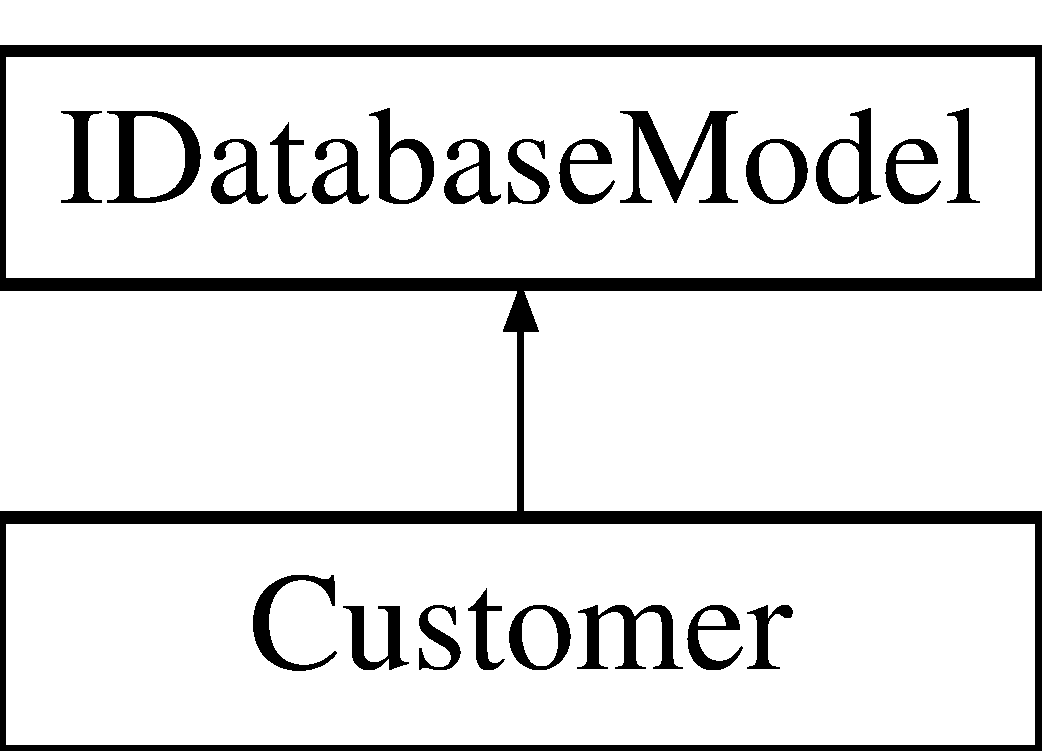
\includegraphics[height=2.000000cm]{d9/d12/classCustomer}
\end{center}
\end{figure}
\subsection*{Public Member Functions}
\begin{DoxyCompactItemize}
\item 
\hypertarget{classCustomer_abcc8fae9701e5ba9d7d6fe44498b34e3}{\hyperlink{classCustomer_abcc8fae9701e5ba9d7d6fe44498b34e3}{Customer} ()}\label{classCustomer_abcc8fae9701e5ba9d7d6fe44498b34e3}

\begin{DoxyCompactList}\small\item\em \hyperlink{classCustomer_abcc8fae9701e5ba9d7d6fe44498b34e3}{Customer\+::\+Customer} Construct a \hyperlink{classCustomer}{Customer}. \end{DoxyCompactList}\item 
\hyperlink{classCustomer_aaea8b3d534c411de73c4fadc26ae114c}{Customer} (int id)
\begin{DoxyCompactList}\small\item\em \hyperlink{classCustomer_abcc8fae9701e5ba9d7d6fe44498b34e3}{Customer\+::\+Customer} Constuct a \hyperlink{classCustomer}{Customer} who is specidied by {\itshape id} \end{DoxyCompactList}\item 
\hypertarget{classCustomer_adcc34b0b12a4d6bf4570f082fef63448}{void \hyperlink{classCustomer_adcc34b0b12a4d6bf4570f082fef63448}{commit} ()}\label{classCustomer_adcc34b0b12a4d6bf4570f082fef63448}

\begin{DoxyCompactList}\small\item\em \hyperlink{classCustomer_adcc34b0b12a4d6bf4570f082fef63448}{Customer\+::commit} Update customer data on the database. \end{DoxyCompactList}\item 
void \hyperlink{classCustomer_ac77f54786ea2bd4c1696c0a76301c639}{hydrat} (int id)
\begin{DoxyCompactList}\small\item\em \hyperlink{classCustomer_ac77f54786ea2bd4c1696c0a76301c639}{Customer\+::hydrat} Insert into database informations related to the \hyperlink{classCustomer}{Customer} who is specified by {\itshape id} \end{DoxyCompactList}\item 
\hypertarget{classCustomer_a8a091ee90fdd7f89a45b28d23c7b834f}{void \hyperlink{classCustomer_a8a091ee90fdd7f89a45b28d23c7b834f}{remove} ()}\label{classCustomer_a8a091ee90fdd7f89a45b28d23c7b834f}

\begin{DoxyCompactList}\small\item\em \hyperlink{classCustomer_a8a091ee90fdd7f89a45b28d23c7b834f}{Customer\+::remove} Remove the current customer. \end{DoxyCompactList}\item 
Q\+String \hyperlink{classCustomer_afda5111886086587dea8b8101bf02fea}{get\+Firstname\+Referent} () const 
\begin{DoxyCompactList}\small\item\em \hyperlink{classCustomer_afda5111886086587dea8b8101bf02fea}{Customer\+::get\+Firstname\+Referent} Return the firstname of the referent \hyperlink{classCustomer}{Customer}. \end{DoxyCompactList}\item 
void \hyperlink{classCustomer_acffda49d2eaf0b0389daa74720887fae}{set\+Firstname\+Referent} (const Q\+String \&firstname\+Referent)
\begin{DoxyCompactList}\small\item\em \hyperlink{classCustomer_acffda49d2eaf0b0389daa74720887fae}{Customer\+::set\+Firstname\+Referent} Replace the referent firstname of the customer by {\itshape firstname\+Referent} \end{DoxyCompactList}\item 
Q\+String \hyperlink{classCustomer_a9232155d920aa83e90fcdae0f4b0f47c}{get\+Lastname\+Referent} () const 
\begin{DoxyCompactList}\small\item\em \hyperlink{classCustomer_a9232155d920aa83e90fcdae0f4b0f47c}{Customer\+::get\+Lastname\+Referent} Return the lastname of the referent \hyperlink{classCustomer}{Customer}. \end{DoxyCompactList}\item 
void \hyperlink{classCustomer_a77d5f5d1c7e6ebc5c1a67adf937f82c0}{set\+Lastname\+Referent} (const Q\+String \&lastname\+Referent)
\begin{DoxyCompactList}\small\item\em Customer\+::set\+Larstname\+Referent Replace the referent lastname of the customer by {\itshape lastname\+Referent} \end{DoxyCompactList}\item 
Q\+String \hyperlink{classCustomer_ae58412194bbc03439aa1bcd387afbe79}{get\+Company} () const 
\begin{DoxyCompactList}\small\item\em \hyperlink{classCustomer_ae58412194bbc03439aa1bcd387afbe79}{Customer\+::get\+Company} Return the name of the company customer. \end{DoxyCompactList}\item 
void \hyperlink{classCustomer_a9d13cc3ad8464df4211da10213821fcc}{set\+Company} (const Q\+String \&company)
\begin{DoxyCompactList}\small\item\em \hyperlink{classCustomer_a9d13cc3ad8464df4211da10213821fcc}{Customer\+::set\+Company} Replace the company name by {\itshape company} \end{DoxyCompactList}\item 
Q\+String \hyperlink{classCustomer_af3e348865143342ad9c67981eb61e0c8}{get\+Address} () const 
\begin{DoxyCompactList}\small\item\em \hyperlink{classCustomer_af3e348865143342ad9c67981eb61e0c8}{Customer\+::get\+Address} Return the address (name and street number) of the customer company. \end{DoxyCompactList}\item 
void \hyperlink{classCustomer_addd0675e408a13f6ab95ec5bd5a3a13b}{set\+Address} (const Q\+String \&address)
\begin{DoxyCompactList}\small\item\em \hyperlink{classCustomer_addd0675e408a13f6ab95ec5bd5a3a13b}{Customer\+::set\+Address} Replace the current company address by the new {\itshape address} \end{DoxyCompactList}\item 
Q\+String \hyperlink{classCustomer_a39073588f2d7669b12a8ecc33b3c4224}{get\+Postal\+Code} () const 
\begin{DoxyCompactList}\small\item\em \hyperlink{classCustomer_a39073588f2d7669b12a8ecc33b3c4224}{Customer\+::get\+Postal\+Code} Return the postal code of the customer company. \end{DoxyCompactList}\item 
void \hyperlink{classCustomer_a3973123c0e94d876124cfdd0444acfd1}{set\+Postal\+Code} (const Q\+String \&postal\+Code)
\begin{DoxyCompactList}\small\item\em \hyperlink{classCustomer_a3973123c0e94d876124cfdd0444acfd1}{Customer\+::set\+Postal\+Code} Replace the current postal code of the customer company by the new {\itshape postal\+Code} \end{DoxyCompactList}\item 
Q\+String \hyperlink{classCustomer_a1eaf38d67a4ac9c8fcc675ff81f724ba}{get\+City} () const 
\begin{DoxyCompactList}\small\item\em \hyperlink{classCustomer_a1eaf38d67a4ac9c8fcc675ff81f724ba}{Customer\+::get\+City} Return the city of the customer company. \end{DoxyCompactList}\item 
void \hyperlink{classCustomer_a1fb29f507135a9f21b29e7799aec14f0}{set\+City} (const Q\+String \&city)
\begin{DoxyCompactList}\small\item\em \hyperlink{classCustomer_a1fb29f507135a9f21b29e7799aec14f0}{Customer\+::set\+City} Replace the current city of the customer company by the new {\itshape city} \end{DoxyCompactList}\item 
Q\+String \hyperlink{classCustomer_a426126096db853802249e10506dc138c}{get\+Country} () const 
\begin{DoxyCompactList}\small\item\em \hyperlink{classCustomer_a426126096db853802249e10506dc138c}{Customer\+::get\+Country} Return the country of the customer company. \end{DoxyCompactList}\item 
void \hyperlink{classCustomer_a81545977d1de88b4ffd6f6b1356ea118}{set\+Country} (const Q\+String \&country)
\begin{DoxyCompactList}\small\item\em \hyperlink{classCustomer_a81545977d1de88b4ffd6f6b1356ea118}{Customer\+::set\+Country} Replace the country of the \hyperlink{classCustomer}{Customer} company by {\itshape country} \end{DoxyCompactList}\item 
Q\+String \hyperlink{classCustomer_a6ab797361537bf4c8b35cce5f1562299}{get\+Email} () const 
\begin{DoxyCompactList}\small\item\em \hyperlink{classCustomer_a6ab797361537bf4c8b35cce5f1562299}{Customer\+::get\+Email} Return the email of the customer company. \end{DoxyCompactList}\item 
void \hyperlink{classCustomer_a64b383efde5855bde7ef385c6f73e45d}{set\+Email} (const Q\+String \&email)
\begin{DoxyCompactList}\small\item\em \hyperlink{classCustomer_a64b383efde5855bde7ef385c6f73e45d}{Customer\+::set\+Email} Replace the email of the \hyperlink{classCustomer}{Customer} company by {\itshape email} \end{DoxyCompactList}\item 
Q\+String \hyperlink{classCustomer_a08546759b1b1f046389bc6ab6b467149}{get\+Mobile\+Phone} () const 
\begin{DoxyCompactList}\small\item\em \hyperlink{classCustomer_a08546759b1b1f046389bc6ab6b467149}{Customer\+::get\+Mobile\+Phone} Return the number of the mobile phone of the customer company. \end{DoxyCompactList}\item 
void \hyperlink{classCustomer_aec562d504cd6c6e3db153544b102e028}{set\+Mobile\+Phone} (const Q\+String \&mobile\+Phone)
\begin{DoxyCompactList}\small\item\em \hyperlink{classCustomer_aec562d504cd6c6e3db153544b102e028}{Customer\+::set\+Mobile\+Phone} Replace the current mobile phone of the customer company by {\itshape mobile\+Phone} \end{DoxyCompactList}\item 
Q\+String \hyperlink{classCustomer_a20b37c158f138def2014f24f291f2aa0}{get\+Phone} () const 
\begin{DoxyCompactList}\small\item\em \hyperlink{classCustomer_a20b37c158f138def2014f24f291f2aa0}{Customer\+::get\+Phone} Return the number of desktop phone. \end{DoxyCompactList}\item 
void \hyperlink{classCustomer_a850d6e8e1a061362928de94553cb12a6}{set\+Phone} (const Q\+String \&phone)
\begin{DoxyCompactList}\small\item\em \hyperlink{classCustomer_a850d6e8e1a061362928de94553cb12a6}{Customer\+::set\+Phone} Replace the current number of desktop phone by {\itshape phone} \end{DoxyCompactList}\item 
Q\+String \hyperlink{classCustomer_ab982339f461136ce230740d776a98ae9}{get\+Fax} () const 
\begin{DoxyCompactList}\small\item\em \hyperlink{classCustomer_ab982339f461136ce230740d776a98ae9}{Customer\+::get\+Fax} Return the fax number. \end{DoxyCompactList}\item 
void \hyperlink{classCustomer_a29049b62abb6aa0733c5def198ed62e5}{set\+Fax} (const Q\+String \&fax)
\begin{DoxyCompactList}\small\item\em \hyperlink{classCustomer_a29049b62abb6aa0733c5def198ed62e5}{Customer\+::set\+Fax} Replace the current fax number by {\itshape fax} \end{DoxyCompactList}\item 
bool \hyperlink{classCustomer_ae55c14b91c08ba15c9593a47931d1949}{operator==} (const \hyperlink{classCustomer}{Customer} \&c)
\begin{DoxyCompactList}\small\item\em \hyperlink{classCustomer_ae55c14b91c08ba15c9593a47931d1949}{Customer\+::operator ==} Re-\/define the operator \char`\"{}==\char`\"{} to compare if the current customer is the same to the other {\bfseries \hyperlink{classCustomer}{Customer}} {\itshape c} Return T\+R\+U\+E if both customers are the same, else F\+A\+L\+S\+E. \end{DoxyCompactList}\item 
bool \hyperlink{classCustomer_a95057d943f370a75c0bfa3d9805b611c}{operator!=} (const \hyperlink{classCustomer}{Customer} \&c)
\begin{DoxyCompactList}\small\item\em \hyperlink{classCustomer_ae55c14b91c08ba15c9593a47931d1949}{Customer\+::operator ==} Re-\/define the operator \char`\"{}!=\char`\"{} to compare if the current customer is differnt to the other {\bfseries \hyperlink{classCustomer}{Customer}} {\itshape c} Return T\+R\+U\+E if both customers are different, else F\+A\+L\+S\+E. \end{DoxyCompactList}\end{DoxyCompactItemize}
\subsection*{Additional Inherited Members}


\subsection{Detailed Description}
The \hyperlink{classCustomer}{Customer} class \hyperlink{classCustomer}{Customer}. 

\begin{DoxyAuthor}{Author}
Antoine de Roquemaurel 

Florent Berbie 
\end{DoxyAuthor}


\subsection{Constructor \& Destructor Documentation}
\hypertarget{classCustomer_aaea8b3d534c411de73c4fadc26ae114c}{\index{Customer@{Customer}!Customer@{Customer}}
\index{Customer@{Customer}!Customer@{Customer}}
\subsubsection[{Customer}]{\setlength{\rightskip}{0pt plus 5cm}Customer\+::\+Customer (
\begin{DoxyParamCaption}
\item[{int}]{id}
\end{DoxyParamCaption}
)}}\label{classCustomer_aaea8b3d534c411de73c4fadc26ae114c}


\hyperlink{classCustomer_abcc8fae9701e5ba9d7d6fe44498b34e3}{Customer\+::\+Customer} Constuct a \hyperlink{classCustomer}{Customer} who is specidied by {\itshape id} 


\begin{DoxyParams}{Parameters}
{\em id} & \hyperlink{classCustomer}{Customer} identify \\
\hline
\end{DoxyParams}


\subsection{Member Function Documentation}
\hypertarget{classCustomer_af3e348865143342ad9c67981eb61e0c8}{\index{Customer@{Customer}!get\+Address@{get\+Address}}
\index{get\+Address@{get\+Address}!Customer@{Customer}}
\subsubsection[{get\+Address}]{\setlength{\rightskip}{0pt plus 5cm}Q\+String Customer\+::get\+Address (
\begin{DoxyParamCaption}
{}
\end{DoxyParamCaption}
) const}}\label{classCustomer_af3e348865143342ad9c67981eb61e0c8}


\hyperlink{classCustomer_af3e348865143342ad9c67981eb61e0c8}{Customer\+::get\+Address} Return the address (name and street number) of the customer company. 

\begin{DoxyReturn}{Returns}
company address 
\end{DoxyReturn}
\hypertarget{classCustomer_a1eaf38d67a4ac9c8fcc675ff81f724ba}{\index{Customer@{Customer}!get\+City@{get\+City}}
\index{get\+City@{get\+City}!Customer@{Customer}}
\subsubsection[{get\+City}]{\setlength{\rightskip}{0pt plus 5cm}Q\+String Customer\+::get\+City (
\begin{DoxyParamCaption}
{}
\end{DoxyParamCaption}
) const}}\label{classCustomer_a1eaf38d67a4ac9c8fcc675ff81f724ba}


\hyperlink{classCustomer_a1eaf38d67a4ac9c8fcc675ff81f724ba}{Customer\+::get\+City} Return the city of the customer company. 

\begin{DoxyReturn}{Returns}
city of the customer company 
\end{DoxyReturn}
\hypertarget{classCustomer_ae58412194bbc03439aa1bcd387afbe79}{\index{Customer@{Customer}!get\+Company@{get\+Company}}
\index{get\+Company@{get\+Company}!Customer@{Customer}}
\subsubsection[{get\+Company}]{\setlength{\rightskip}{0pt plus 5cm}Q\+String Customer\+::get\+Company (
\begin{DoxyParamCaption}
{}
\end{DoxyParamCaption}
) const}}\label{classCustomer_ae58412194bbc03439aa1bcd387afbe79}


\hyperlink{classCustomer_ae58412194bbc03439aa1bcd387afbe79}{Customer\+::get\+Company} Return the name of the company customer. 

\begin{DoxyReturn}{Returns}
name of the company customer 
\end{DoxyReturn}
\hypertarget{classCustomer_a426126096db853802249e10506dc138c}{\index{Customer@{Customer}!get\+Country@{get\+Country}}
\index{get\+Country@{get\+Country}!Customer@{Customer}}
\subsubsection[{get\+Country}]{\setlength{\rightskip}{0pt plus 5cm}Q\+String Customer\+::get\+Country (
\begin{DoxyParamCaption}
{}
\end{DoxyParamCaption}
) const}}\label{classCustomer_a426126096db853802249e10506dc138c}


\hyperlink{classCustomer_a426126096db853802249e10506dc138c}{Customer\+::get\+Country} Return the country of the customer company. 

\begin{DoxyReturn}{Returns}
country of the customer company 
\end{DoxyReturn}
\hypertarget{classCustomer_a6ab797361537bf4c8b35cce5f1562299}{\index{Customer@{Customer}!get\+Email@{get\+Email}}
\index{get\+Email@{get\+Email}!Customer@{Customer}}
\subsubsection[{get\+Email}]{\setlength{\rightskip}{0pt plus 5cm}Q\+String Customer\+::get\+Email (
\begin{DoxyParamCaption}
{}
\end{DoxyParamCaption}
) const}}\label{classCustomer_a6ab797361537bf4c8b35cce5f1562299}


\hyperlink{classCustomer_a6ab797361537bf4c8b35cce5f1562299}{Customer\+::get\+Email} Return the email of the customer company. 

\begin{DoxyReturn}{Returns}
email of the customer company 
\end{DoxyReturn}
\hypertarget{classCustomer_ab982339f461136ce230740d776a98ae9}{\index{Customer@{Customer}!get\+Fax@{get\+Fax}}
\index{get\+Fax@{get\+Fax}!Customer@{Customer}}
\subsubsection[{get\+Fax}]{\setlength{\rightskip}{0pt plus 5cm}Q\+String Customer\+::get\+Fax (
\begin{DoxyParamCaption}
{}
\end{DoxyParamCaption}
) const}}\label{classCustomer_ab982339f461136ce230740d776a98ae9}


\hyperlink{classCustomer_ab982339f461136ce230740d776a98ae9}{Customer\+::get\+Fax} Return the fax number. 

\begin{DoxyReturn}{Returns}
fax number 
\end{DoxyReturn}
\hypertarget{classCustomer_afda5111886086587dea8b8101bf02fea}{\index{Customer@{Customer}!get\+Firstname\+Referent@{get\+Firstname\+Referent}}
\index{get\+Firstname\+Referent@{get\+Firstname\+Referent}!Customer@{Customer}}
\subsubsection[{get\+Firstname\+Referent}]{\setlength{\rightskip}{0pt plus 5cm}Q\+String Customer\+::get\+Firstname\+Referent (
\begin{DoxyParamCaption}
{}
\end{DoxyParamCaption}
) const}}\label{classCustomer_afda5111886086587dea8b8101bf02fea}


\hyperlink{classCustomer_afda5111886086587dea8b8101bf02fea}{Customer\+::get\+Firstname\+Referent} Return the firstname of the referent \hyperlink{classCustomer}{Customer}. 

\begin{DoxyReturn}{Returns}
Referent firstname of the customer 
\end{DoxyReturn}
\hypertarget{classCustomer_a9232155d920aa83e90fcdae0f4b0f47c}{\index{Customer@{Customer}!get\+Lastname\+Referent@{get\+Lastname\+Referent}}
\index{get\+Lastname\+Referent@{get\+Lastname\+Referent}!Customer@{Customer}}
\subsubsection[{get\+Lastname\+Referent}]{\setlength{\rightskip}{0pt plus 5cm}Q\+String Customer\+::get\+Lastname\+Referent (
\begin{DoxyParamCaption}
{}
\end{DoxyParamCaption}
) const}}\label{classCustomer_a9232155d920aa83e90fcdae0f4b0f47c}


\hyperlink{classCustomer_a9232155d920aa83e90fcdae0f4b0f47c}{Customer\+::get\+Lastname\+Referent} Return the lastname of the referent \hyperlink{classCustomer}{Customer}. 

\begin{DoxyReturn}{Returns}
Referent lastname of the customer 
\end{DoxyReturn}
\hypertarget{classCustomer_a08546759b1b1f046389bc6ab6b467149}{\index{Customer@{Customer}!get\+Mobile\+Phone@{get\+Mobile\+Phone}}
\index{get\+Mobile\+Phone@{get\+Mobile\+Phone}!Customer@{Customer}}
\subsubsection[{get\+Mobile\+Phone}]{\setlength{\rightskip}{0pt plus 5cm}Q\+String Customer\+::get\+Mobile\+Phone (
\begin{DoxyParamCaption}
{}
\end{DoxyParamCaption}
) const}}\label{classCustomer_a08546759b1b1f046389bc6ab6b467149}


\hyperlink{classCustomer_a08546759b1b1f046389bc6ab6b467149}{Customer\+::get\+Mobile\+Phone} Return the number of the mobile phone of the customer company. 

\begin{DoxyReturn}{Returns}
number of mobile phone 
\end{DoxyReturn}
\hypertarget{classCustomer_a20b37c158f138def2014f24f291f2aa0}{\index{Customer@{Customer}!get\+Phone@{get\+Phone}}
\index{get\+Phone@{get\+Phone}!Customer@{Customer}}
\subsubsection[{get\+Phone}]{\setlength{\rightskip}{0pt plus 5cm}Q\+String Customer\+::get\+Phone (
\begin{DoxyParamCaption}
{}
\end{DoxyParamCaption}
) const}}\label{classCustomer_a20b37c158f138def2014f24f291f2aa0}


\hyperlink{classCustomer_a20b37c158f138def2014f24f291f2aa0}{Customer\+::get\+Phone} Return the number of desktop phone. 

\begin{DoxyReturn}{Returns}
number of desktop phone 
\end{DoxyReturn}
\hypertarget{classCustomer_a39073588f2d7669b12a8ecc33b3c4224}{\index{Customer@{Customer}!get\+Postal\+Code@{get\+Postal\+Code}}
\index{get\+Postal\+Code@{get\+Postal\+Code}!Customer@{Customer}}
\subsubsection[{get\+Postal\+Code}]{\setlength{\rightskip}{0pt plus 5cm}Q\+String Customer\+::get\+Postal\+Code (
\begin{DoxyParamCaption}
{}
\end{DoxyParamCaption}
) const}}\label{classCustomer_a39073588f2d7669b12a8ecc33b3c4224}


\hyperlink{classCustomer_a39073588f2d7669b12a8ecc33b3c4224}{Customer\+::get\+Postal\+Code} Return the postal code of the customer company. 

\begin{DoxyReturn}{Returns}
postal code of the customer company 
\end{DoxyReturn}
\hypertarget{classCustomer_ac77f54786ea2bd4c1696c0a76301c639}{\index{Customer@{Customer}!hydrat@{hydrat}}
\index{hydrat@{hydrat}!Customer@{Customer}}
\subsubsection[{hydrat}]{\setlength{\rightskip}{0pt plus 5cm}void Customer\+::hydrat (
\begin{DoxyParamCaption}
\item[{int}]{id}
\end{DoxyParamCaption}
)\hspace{0.3cm}{\ttfamily [virtual]}}}\label{classCustomer_ac77f54786ea2bd4c1696c0a76301c639}


\hyperlink{classCustomer_ac77f54786ea2bd4c1696c0a76301c639}{Customer\+::hydrat} Insert into database informations related to the \hyperlink{classCustomer}{Customer} who is specified by {\itshape id} 


\begin{DoxyParams}{Parameters}
{\em id} & \hyperlink{classCustomer}{Customer} identify \\
\hline
\end{DoxyParams}


Implements \hyperlink{classIDatabaseModel_a25e44ed10a75976f86e14d34aea02c37}{I\+Database\+Model}.

\hypertarget{classCustomer_a95057d943f370a75c0bfa3d9805b611c}{\index{Customer@{Customer}!operator"!=@{operator"!=}}
\index{operator"!=@{operator"!=}!Customer@{Customer}}
\subsubsection[{operator"!=}]{\setlength{\rightskip}{0pt plus 5cm}bool Customer\+::operator!= (
\begin{DoxyParamCaption}
\item[{const {\bf Customer} \&}]{c}
\end{DoxyParamCaption}
)}}\label{classCustomer_a95057d943f370a75c0bfa3d9805b611c}


\hyperlink{classCustomer_ae55c14b91c08ba15c9593a47931d1949}{Customer\+::operator ==} Re-\/define the operator \char`\"{}!=\char`\"{} to compare if the current customer is differnt to the other {\bfseries \hyperlink{classCustomer}{Customer}} {\itshape c} Return T\+R\+U\+E if both customers are different, else F\+A\+L\+S\+E. 


\begin{DoxyParams}{Parameters}
{\em c} & \hyperlink{classCustomer}{Customer} to compare \\
\hline
\end{DoxyParams}
\begin{DoxyReturn}{Returns}
boolean 
\end{DoxyReturn}
\hypertarget{classCustomer_ae55c14b91c08ba15c9593a47931d1949}{\index{Customer@{Customer}!operator==@{operator==}}
\index{operator==@{operator==}!Customer@{Customer}}
\subsubsection[{operator==}]{\setlength{\rightskip}{0pt plus 5cm}bool Customer\+::operator== (
\begin{DoxyParamCaption}
\item[{const {\bf Customer} \&}]{c}
\end{DoxyParamCaption}
)}}\label{classCustomer_ae55c14b91c08ba15c9593a47931d1949}


\hyperlink{classCustomer_ae55c14b91c08ba15c9593a47931d1949}{Customer\+::operator ==} Re-\/define the operator \char`\"{}==\char`\"{} to compare if the current customer is the same to the other {\bfseries \hyperlink{classCustomer}{Customer}} {\itshape c} Return T\+R\+U\+E if both customers are the same, else F\+A\+L\+S\+E. 


\begin{DoxyParams}{Parameters}
{\em c} & \hyperlink{classCustomer}{Customer} to compare \\
\hline
\end{DoxyParams}
\begin{DoxyReturn}{Returns}
boolean 
\end{DoxyReturn}
\hypertarget{classCustomer_addd0675e408a13f6ab95ec5bd5a3a13b}{\index{Customer@{Customer}!set\+Address@{set\+Address}}
\index{set\+Address@{set\+Address}!Customer@{Customer}}
\subsubsection[{set\+Address}]{\setlength{\rightskip}{0pt plus 5cm}void Customer\+::set\+Address (
\begin{DoxyParamCaption}
\item[{const Q\+String \&}]{address}
\end{DoxyParamCaption}
)}}\label{classCustomer_addd0675e408a13f6ab95ec5bd5a3a13b}


\hyperlink{classCustomer_addd0675e408a13f6ab95ec5bd5a3a13b}{Customer\+::set\+Address} Replace the current company address by the new {\itshape address} 


\begin{DoxyParams}{Parameters}
{\em address} & New company address \\
\hline
\end{DoxyParams}
\hypertarget{classCustomer_a1fb29f507135a9f21b29e7799aec14f0}{\index{Customer@{Customer}!set\+City@{set\+City}}
\index{set\+City@{set\+City}!Customer@{Customer}}
\subsubsection[{set\+City}]{\setlength{\rightskip}{0pt plus 5cm}void Customer\+::set\+City (
\begin{DoxyParamCaption}
\item[{const Q\+String \&}]{city}
\end{DoxyParamCaption}
)}}\label{classCustomer_a1fb29f507135a9f21b29e7799aec14f0}


\hyperlink{classCustomer_a1fb29f507135a9f21b29e7799aec14f0}{Customer\+::set\+City} Replace the current city of the customer company by the new {\itshape city} 


\begin{DoxyParams}{Parameters}
{\em city} & New city of the customer company \\
\hline
\end{DoxyParams}
\hypertarget{classCustomer_a9d13cc3ad8464df4211da10213821fcc}{\index{Customer@{Customer}!set\+Company@{set\+Company}}
\index{set\+Company@{set\+Company}!Customer@{Customer}}
\subsubsection[{set\+Company}]{\setlength{\rightskip}{0pt plus 5cm}void Customer\+::set\+Company (
\begin{DoxyParamCaption}
\item[{const Q\+String \&}]{company}
\end{DoxyParamCaption}
)}}\label{classCustomer_a9d13cc3ad8464df4211da10213821fcc}


\hyperlink{classCustomer_a9d13cc3ad8464df4211da10213821fcc}{Customer\+::set\+Company} Replace the company name by {\itshape company} 


\begin{DoxyParams}{Parameters}
{\em company} & New company name \\
\hline
\end{DoxyParams}
\hypertarget{classCustomer_a81545977d1de88b4ffd6f6b1356ea118}{\index{Customer@{Customer}!set\+Country@{set\+Country}}
\index{set\+Country@{set\+Country}!Customer@{Customer}}
\subsubsection[{set\+Country}]{\setlength{\rightskip}{0pt plus 5cm}void Customer\+::set\+Country (
\begin{DoxyParamCaption}
\item[{const Q\+String \&}]{country}
\end{DoxyParamCaption}
)}}\label{classCustomer_a81545977d1de88b4ffd6f6b1356ea118}


\hyperlink{classCustomer_a81545977d1de88b4ffd6f6b1356ea118}{Customer\+::set\+Country} Replace the country of the \hyperlink{classCustomer}{Customer} company by {\itshape country} 


\begin{DoxyParams}{Parameters}
{\em country} & New country of the customer company \\
\hline
\end{DoxyParams}
\hypertarget{classCustomer_a64b383efde5855bde7ef385c6f73e45d}{\index{Customer@{Customer}!set\+Email@{set\+Email}}
\index{set\+Email@{set\+Email}!Customer@{Customer}}
\subsubsection[{set\+Email}]{\setlength{\rightskip}{0pt plus 5cm}void Customer\+::set\+Email (
\begin{DoxyParamCaption}
\item[{const Q\+String \&}]{email}
\end{DoxyParamCaption}
)}}\label{classCustomer_a64b383efde5855bde7ef385c6f73e45d}


\hyperlink{classCustomer_a64b383efde5855bde7ef385c6f73e45d}{Customer\+::set\+Email} Replace the email of the \hyperlink{classCustomer}{Customer} company by {\itshape email} 


\begin{DoxyParams}{Parameters}
{\em email} & New email of the customer company \\
\hline
\end{DoxyParams}
\hypertarget{classCustomer_a29049b62abb6aa0733c5def198ed62e5}{\index{Customer@{Customer}!set\+Fax@{set\+Fax}}
\index{set\+Fax@{set\+Fax}!Customer@{Customer}}
\subsubsection[{set\+Fax}]{\setlength{\rightskip}{0pt plus 5cm}void Customer\+::set\+Fax (
\begin{DoxyParamCaption}
\item[{const Q\+String \&}]{fax}
\end{DoxyParamCaption}
)}}\label{classCustomer_a29049b62abb6aa0733c5def198ed62e5}


\hyperlink{classCustomer_a29049b62abb6aa0733c5def198ed62e5}{Customer\+::set\+Fax} Replace the current fax number by {\itshape fax} 


\begin{DoxyParams}{Parameters}
{\em fax} & new fax number \\
\hline
\end{DoxyParams}
\hypertarget{classCustomer_acffda49d2eaf0b0389daa74720887fae}{\index{Customer@{Customer}!set\+Firstname\+Referent@{set\+Firstname\+Referent}}
\index{set\+Firstname\+Referent@{set\+Firstname\+Referent}!Customer@{Customer}}
\subsubsection[{set\+Firstname\+Referent}]{\setlength{\rightskip}{0pt plus 5cm}void Customer\+::set\+Firstname\+Referent (
\begin{DoxyParamCaption}
\item[{const Q\+String \&}]{firstname\+Referent}
\end{DoxyParamCaption}
)}}\label{classCustomer_acffda49d2eaf0b0389daa74720887fae}


\hyperlink{classCustomer_acffda49d2eaf0b0389daa74720887fae}{Customer\+::set\+Firstname\+Referent} Replace the referent firstname of the customer by {\itshape firstname\+Referent} 


\begin{DoxyParams}{Parameters}
{\em firstname\+Referent} & New referent firstname of the \hyperlink{classCustomer}{Customer} \\
\hline
\end{DoxyParams}
\hypertarget{classCustomer_a77d5f5d1c7e6ebc5c1a67adf937f82c0}{\index{Customer@{Customer}!set\+Lastname\+Referent@{set\+Lastname\+Referent}}
\index{set\+Lastname\+Referent@{set\+Lastname\+Referent}!Customer@{Customer}}
\subsubsection[{set\+Lastname\+Referent}]{\setlength{\rightskip}{0pt plus 5cm}void Customer\+::set\+Lastname\+Referent (
\begin{DoxyParamCaption}
\item[{const Q\+String \&}]{lastname\+Referent}
\end{DoxyParamCaption}
)}}\label{classCustomer_a77d5f5d1c7e6ebc5c1a67adf937f82c0}


Customer\+::set\+Larstname\+Referent Replace the referent lastname of the customer by {\itshape lastname\+Referent} 


\begin{DoxyParams}{Parameters}
{\em lastname\+Referent} & New referent lastname of the \hyperlink{classCustomer}{Customer} \\
\hline
\end{DoxyParams}
\hypertarget{classCustomer_aec562d504cd6c6e3db153544b102e028}{\index{Customer@{Customer}!set\+Mobile\+Phone@{set\+Mobile\+Phone}}
\index{set\+Mobile\+Phone@{set\+Mobile\+Phone}!Customer@{Customer}}
\subsubsection[{set\+Mobile\+Phone}]{\setlength{\rightskip}{0pt plus 5cm}void Customer\+::set\+Mobile\+Phone (
\begin{DoxyParamCaption}
\item[{const Q\+String \&}]{mobile\+Phone}
\end{DoxyParamCaption}
)}}\label{classCustomer_aec562d504cd6c6e3db153544b102e028}


\hyperlink{classCustomer_aec562d504cd6c6e3db153544b102e028}{Customer\+::set\+Mobile\+Phone} Replace the current mobile phone of the customer company by {\itshape mobile\+Phone} 


\begin{DoxyParams}{Parameters}
{\em mobile\+Phone} & New number of mobile phone \\
\hline
\end{DoxyParams}
\hypertarget{classCustomer_a850d6e8e1a061362928de94553cb12a6}{\index{Customer@{Customer}!set\+Phone@{set\+Phone}}
\index{set\+Phone@{set\+Phone}!Customer@{Customer}}
\subsubsection[{set\+Phone}]{\setlength{\rightskip}{0pt plus 5cm}void Customer\+::set\+Phone (
\begin{DoxyParamCaption}
\item[{const Q\+String \&}]{phone}
\end{DoxyParamCaption}
)}}\label{classCustomer_a850d6e8e1a061362928de94553cb12a6}


\hyperlink{classCustomer_a850d6e8e1a061362928de94553cb12a6}{Customer\+::set\+Phone} Replace the current number of desktop phone by {\itshape phone} 


\begin{DoxyParams}{Parameters}
{\em phone} & New number of desktop phone \\
\hline
\end{DoxyParams}
\hypertarget{classCustomer_a3973123c0e94d876124cfdd0444acfd1}{\index{Customer@{Customer}!set\+Postal\+Code@{set\+Postal\+Code}}
\index{set\+Postal\+Code@{set\+Postal\+Code}!Customer@{Customer}}
\subsubsection[{set\+Postal\+Code}]{\setlength{\rightskip}{0pt plus 5cm}void Customer\+::set\+Postal\+Code (
\begin{DoxyParamCaption}
\item[{const Q\+String \&}]{postal\+Code}
\end{DoxyParamCaption}
)}}\label{classCustomer_a3973123c0e94d876124cfdd0444acfd1}


\hyperlink{classCustomer_a3973123c0e94d876124cfdd0444acfd1}{Customer\+::set\+Postal\+Code} Replace the current postal code of the customer company by the new {\itshape postal\+Code} 


\begin{DoxyParams}{Parameters}
{\em postal\+Code} & New postal code of the customer company \\
\hline
\end{DoxyParams}


The documentation for this class was generated from the following files\+:\begin{DoxyCompactItemize}
\item 
src/models/customer.\+h\item 
src/models/customer.\+cpp\end{DoxyCompactItemize}

\hypertarget{classCustomerContextualMenu}{\section{Customer\+Contextual\+Menu Class Reference}
\label{classCustomerContextualMenu}\index{Customer\+Contextual\+Menu@{Customer\+Contextual\+Menu}}
}


Display contextual menu on a customer.  




{\ttfamily \#include $<$customercontextualmenu.\+h$>$}

Inheritance diagram for Customer\+Contextual\+Menu\+:\begin{figure}[H]
\begin{center}
\leavevmode
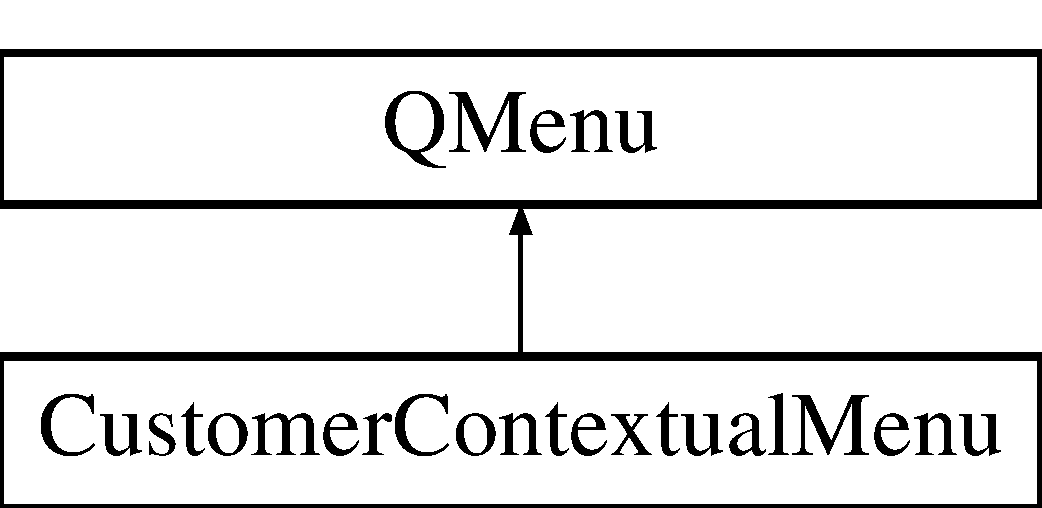
\includegraphics[height=2.000000cm]{d5/db9/classCustomerContextualMenu}
\end{center}
\end{figure}
\subsection*{Public Member Functions}
\begin{DoxyCompactItemize}
\item 
\hypertarget{classCustomerContextualMenu_a798a08f4b8526398a54752e7de87930e}{{\bfseries Customer\+Contextual\+Menu} (Q\+Widget $\ast$w=0)}\label{classCustomerContextualMenu_a798a08f4b8526398a54752e7de87930e}

\end{DoxyCompactItemize}


\subsection{Detailed Description}
Display contextual menu on a customer. 

\begin{DoxyAuthor}{Author}
Antoine de Roquemaurel 
\end{DoxyAuthor}


The documentation for this class was generated from the following files\+:\begin{DoxyCompactItemize}
\item 
src/widgets/customercontextualmenu.\+h\item 
src/widgets/customercontextualmenu.\+cpp\end{DoxyCompactItemize}

\hypertarget{classCustomerDatabase}{\section{Customer\-Database Class Reference}
\label{classCustomerDatabase}\index{Customer\-Database@{Customer\-Database}}
}


The {\bfseries \hyperlink{classCustomerDatabase}{Customer\-Database}} class \hyperlink{classCustomer}{Customer} table database.  




{\ttfamily \#include $<$customerdatabase.\-h$>$}

Inheritance diagram for Customer\-Database\-:\begin{figure}[H]
\begin{center}
\leavevmode
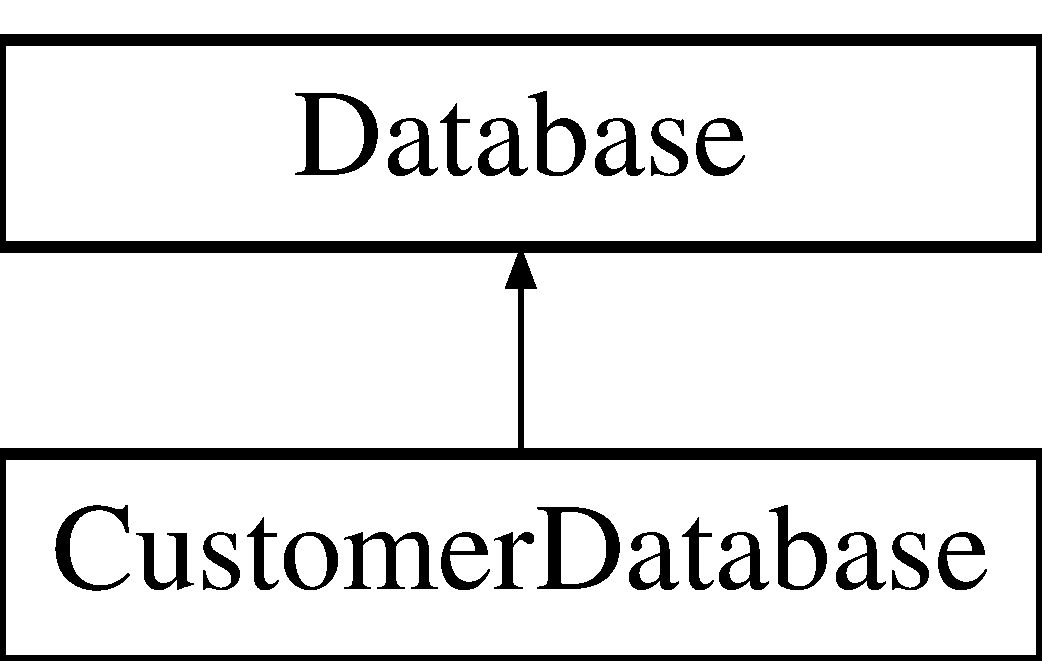
\includegraphics[height=2.000000cm]{dc/d7c/classCustomerDatabase}
\end{center}
\end{figure}
\subsection*{Public Member Functions}
\begin{DoxyCompactItemize}
\item 
Q\-Standard\-Item\-Model $\ast$ \hyperlink{classCustomerDatabase_a2e25b4f197ccbdd2c5753558dbe18d4b}{get\-Customers\-Table} (Q\-String filter=\char`\"{}\char`\"{})  throw (\-Db\-Exception$\ast$)
\begin{DoxyCompactList}\small\item\em \hyperlink{classCustomerDatabase_a2e25b4f197ccbdd2c5753558dbe18d4b}{Customer\-Database\-::get\-Customers\-Table} Return an item model of customers for Q\-Table\-View. \end{DoxyCompactList}\item 
Q\-Standard\-Item\-Model $\ast$ \hyperlink{classCustomerDatabase_a0fc1ca7fe1020cef19b2423531c4e934}{get\-Customers\-Tree} (Q\-String filter=\char`\"{}\char`\"{})  throw (\-Db\-Exception$\ast$)
\begin{DoxyCompactList}\small\item\em \hyperlink{classCustomerDatabase_a0fc1ca7fe1020cef19b2423531c4e934}{Customer\-Database\-::get\-Customers\-Tree} Return an item model of customers for Q\-Tree. \end{DoxyCompactList}\item 
\hyperlink{classCustomer}{Customer} $\ast$ \hyperlink{classCustomerDatabase_ae510e11ab1efe33b8e1da21bc1ca6f2d}{get\-Customer} (const int p\-Id)
\begin{DoxyCompactList}\small\item\em \hyperlink{classCustomerDatabase_ae510e11ab1efe33b8e1da21bc1ca6f2d}{Customer\-Database\-::get\-Customer} get informations about the customer identified by {\itshape p\-Id} \end{DoxyCompactList}\item 
int \hyperlink{classCustomerDatabase_a522337809fe7588ddc8b5eb27b0cb640}{add\-Customer} (const \hyperlink{classCustomer}{Customer} \&)
\begin{DoxyCompactList}\small\item\em \hyperlink{classCustomerDatabase_a522337809fe7588ddc8b5eb27b0cb640}{Customer\-Database\-::add\-Customer} Add the customer {\itshape p\-Customer} to the database. \end{DoxyCompactList}\item 
\hypertarget{classCustomerDatabase_a2ae17af9bcbf889dec21b4acae3161e1}{void \hyperlink{classCustomerDatabase_a2ae17af9bcbf889dec21b4acae3161e1}{update\-Customer} (const \hyperlink{classCustomer}{Customer} \&)}\label{classCustomerDatabase_a2ae17af9bcbf889dec21b4acae3161e1}

\begin{DoxyCompactList}\small\item\em \hyperlink{classCustomerDatabase_a2ae17af9bcbf889dec21b4acae3161e1}{Customer\-Database\-::update\-Customer} Update informations about the customer {\itshape p\-Customer} \end{DoxyCompactList}\item 
void \hyperlink{classCustomerDatabase_aa1d21765bdf6319e580b3fcf20d841d1}{remove\-Customer} (const int p\-Id)
\begin{DoxyCompactList}\small\item\em \hyperlink{classCustomerDatabase_aa1d21765bdf6319e580b3fcf20d841d1}{Customer\-Database\-::remove\-Customer} Remove the customer with the id {\itshape p\-Id} \end{DoxyCompactList}\item 
int \hyperlink{classCustomerDatabase_a1c60ecbaa2594426b522746c70beee19}{get\-Nb\-Customers} ()
\begin{DoxyCompactList}\small\item\em \hyperlink{classCustomerDatabase_a1c60ecbaa2594426b522746c70beee19}{Customer\-Database\-::get\-Nb\-Customers} Return the number of customers existing. \end{DoxyCompactList}\end{DoxyCompactItemize}
\subsection*{Static Public Member Functions}
\begin{DoxyCompactItemize}
\item 
static \hyperlink{classCustomerDatabase}{Customer\-Database} $\ast$ \hyperlink{classCustomerDatabase_a2b9546b1e5803c4055529d2a7f7df95e}{instance} ()  throw (\-Db\-Exception$\ast$)
\begin{DoxyCompactList}\small\item\em Customer\-Database\-::get\-Instance Return an instance of {\bfseries \hyperlink{classCustomerDatabase}{Customer\-Database}} \end{DoxyCompactList}\end{DoxyCompactItemize}
\subsection*{Additional Inherited Members}


\subsection{Detailed Description}
The {\bfseries \hyperlink{classCustomerDatabase}{Customer\-Database}} class \hyperlink{classCustomer}{Customer} table database. 

\begin{DoxyAuthor}{Author}
Antoine de Roquemaurel 
\end{DoxyAuthor}
\begin{DoxySeeAlso}{See Also}
\hyperlink{classDatabase}{Database} 

\hyperlink{classCustomer}{Customer} 
\end{DoxySeeAlso}


\subsection{Member Function Documentation}
\hypertarget{classCustomerDatabase_a522337809fe7588ddc8b5eb27b0cb640}{\index{Customer\-Database@{Customer\-Database}!add\-Customer@{add\-Customer}}
\index{add\-Customer@{add\-Customer}!CustomerDatabase@{Customer\-Database}}
\subsubsection[{add\-Customer}]{\setlength{\rightskip}{0pt plus 5cm}int Customer\-Database\-::add\-Customer (
\begin{DoxyParamCaption}
\item[{const {\bf Customer} \&}]{p\-Customer}
\end{DoxyParamCaption}
)}}\label{classCustomerDatabase_a522337809fe7588ddc8b5eb27b0cb640}


\hyperlink{classCustomerDatabase_a522337809fe7588ddc8b5eb27b0cb640}{Customer\-Database\-::add\-Customer} Add the customer {\itshape p\-Customer} to the database. 

\begin{DoxyReturn}{Returns}
customer id 
\end{DoxyReturn}
\hypertarget{classCustomerDatabase_ae510e11ab1efe33b8e1da21bc1ca6f2d}{\index{Customer\-Database@{Customer\-Database}!get\-Customer@{get\-Customer}}
\index{get\-Customer@{get\-Customer}!CustomerDatabase@{Customer\-Database}}
\subsubsection[{get\-Customer}]{\setlength{\rightskip}{0pt plus 5cm}{\bf Customer} $\ast$ Customer\-Database\-::get\-Customer (
\begin{DoxyParamCaption}
\item[{const int}]{p\-Id}
\end{DoxyParamCaption}
)}}\label{classCustomerDatabase_ae510e11ab1efe33b8e1da21bc1ca6f2d}


\hyperlink{classCustomerDatabase_ae510e11ab1efe33b8e1da21bc1ca6f2d}{Customer\-Database\-::get\-Customer} get informations about the customer identified by {\itshape p\-Id} 


\begin{DoxyParams}{Parameters}
{\em p\-Id} & customer id \\
\hline
\end{DoxyParams}
\begin{DoxyReturn}{Returns}
the \hyperlink{classCustomer}{Customer} 
\end{DoxyReturn}
\hypertarget{classCustomerDatabase_a2e25b4f197ccbdd2c5753558dbe18d4b}{\index{Customer\-Database@{Customer\-Database}!get\-Customers\-Table@{get\-Customers\-Table}}
\index{get\-Customers\-Table@{get\-Customers\-Table}!CustomerDatabase@{Customer\-Database}}
\subsubsection[{get\-Customers\-Table}]{\setlength{\rightskip}{0pt plus 5cm}Q\-Standard\-Item\-Model $\ast$ Customer\-Database\-::get\-Customers\-Table (
\begin{DoxyParamCaption}
\item[{Q\-String}]{filter = {\ttfamily \char`\"{}\char`\"{}}}
\end{DoxyParamCaption}
) throw  {\bf Db\-Exception} $\ast$) }}\label{classCustomerDatabase_a2e25b4f197ccbdd2c5753558dbe18d4b}


\hyperlink{classCustomerDatabase_a2e25b4f197ccbdd2c5753558dbe18d4b}{Customer\-Database\-::get\-Customers\-Table} Return an item model of customers for Q\-Table\-View. 

\begin{DoxyAuthor}{Author}
Manantsoa Razanajatovo 
\end{DoxyAuthor}

\begin{DoxyParams}{Parameters}
{\em filter} & Select only customers who are specified by {\itshape filter} \\
\hline
\end{DoxyParams}

\begin{DoxyExceptions}{Exceptions}
{\em \hyperlink{classDbException}{Db\-Exception}} & \\
\hline
\end{DoxyExceptions}
\begin{DoxyReturn}{Returns}
Q\-Standard\-Item\-Model an item model for Q\-Table\-View 
\end{DoxyReturn}
\hypertarget{classCustomerDatabase_a0fc1ca7fe1020cef19b2423531c4e934}{\index{Customer\-Database@{Customer\-Database}!get\-Customers\-Tree@{get\-Customers\-Tree}}
\index{get\-Customers\-Tree@{get\-Customers\-Tree}!CustomerDatabase@{Customer\-Database}}
\subsubsection[{get\-Customers\-Tree}]{\setlength{\rightskip}{0pt plus 5cm}Q\-Standard\-Item\-Model $\ast$ Customer\-Database\-::get\-Customers\-Tree (
\begin{DoxyParamCaption}
\item[{Q\-String}]{filter = {\ttfamily \char`\"{}\char`\"{}}}
\end{DoxyParamCaption}
) throw  {\bf Db\-Exception} $\ast$) }}\label{classCustomerDatabase_a0fc1ca7fe1020cef19b2423531c4e934}


\hyperlink{classCustomerDatabase_a0fc1ca7fe1020cef19b2423531c4e934}{Customer\-Database\-::get\-Customers\-Tree} Return an item model of customers for Q\-Tree. 

\begin{DoxyAuthor}{Author}
Manantsoa Razanajatovo 
\end{DoxyAuthor}

\begin{DoxyParams}{Parameters}
{\em filter} & Select only customers who are specified by {\itshape filter} \\
\hline
\end{DoxyParams}

\begin{DoxyExceptions}{Exceptions}
{\em \hyperlink{classDbException}{Db\-Exception}} & \\
\hline
\end{DoxyExceptions}
\begin{DoxyReturn}{Returns}
Q\-Standard\-Item\-Model an item model for Q\-Table\-View 
\end{DoxyReturn}
\hypertarget{classCustomerDatabase_a1c60ecbaa2594426b522746c70beee19}{\index{Customer\-Database@{Customer\-Database}!get\-Nb\-Customers@{get\-Nb\-Customers}}
\index{get\-Nb\-Customers@{get\-Nb\-Customers}!CustomerDatabase@{Customer\-Database}}
\subsubsection[{get\-Nb\-Customers}]{\setlength{\rightskip}{0pt plus 5cm}int Customer\-Database\-::get\-Nb\-Customers (
\begin{DoxyParamCaption}
{}
\end{DoxyParamCaption}
)}}\label{classCustomerDatabase_a1c60ecbaa2594426b522746c70beee19}


\hyperlink{classCustomerDatabase_a1c60ecbaa2594426b522746c70beee19}{Customer\-Database\-::get\-Nb\-Customers} Return the number of customers existing. 

\begin{DoxyReturn}{Returns}
number of customers 
\end{DoxyReturn}
\hypertarget{classCustomerDatabase_a2b9546b1e5803c4055529d2a7f7df95e}{\index{Customer\-Database@{Customer\-Database}!instance@{instance}}
\index{instance@{instance}!CustomerDatabase@{Customer\-Database}}
\subsubsection[{instance}]{\setlength{\rightskip}{0pt plus 5cm}{\bf Customer\-Database} $\ast$ Customer\-Database\-::instance (
\begin{DoxyParamCaption}
{}
\end{DoxyParamCaption}
) throw  {\bf Db\-Exception} $\ast$) \hspace{0.3cm}{\ttfamily [static]}}}\label{classCustomerDatabase_a2b9546b1e5803c4055529d2a7f7df95e}


Customer\-Database\-::get\-Instance Return an instance of {\bfseries \hyperlink{classCustomerDatabase}{Customer\-Database}} 

\begin{DoxySeeAlso}{See Also}
\hyperlink{classDbException}{Db\-Exception} 
\end{DoxySeeAlso}
\begin{DoxyReturn}{Returns}
Instance of \hyperlink{classCustomerDatabase}{Customer\-Database} 
\end{DoxyReturn}
\hypertarget{classCustomerDatabase_aa1d21765bdf6319e580b3fcf20d841d1}{\index{Customer\-Database@{Customer\-Database}!remove\-Customer@{remove\-Customer}}
\index{remove\-Customer@{remove\-Customer}!CustomerDatabase@{Customer\-Database}}
\subsubsection[{remove\-Customer}]{\setlength{\rightskip}{0pt plus 5cm}void Customer\-Database\-::remove\-Customer (
\begin{DoxyParamCaption}
\item[{const int}]{p\-Id}
\end{DoxyParamCaption}
)}}\label{classCustomerDatabase_aa1d21765bdf6319e580b3fcf20d841d1}


\hyperlink{classCustomerDatabase_aa1d21765bdf6319e580b3fcf20d841d1}{Customer\-Database\-::remove\-Customer} Remove the customer with the id {\itshape p\-Id} 


\begin{DoxyParams}{Parameters}
{\em p\-Id} & customer id \\
\hline
\end{DoxyParams}


The documentation for this class was generated from the following files\-:\begin{DoxyCompactItemize}
\item 
/home/florent/\-Documents/\-Projet\-\_\-\-S8/\-Fact\-Dev/src/database/customerdatabase.\-h\item 
/home/florent/\-Documents/\-Projet\-\_\-\-S8/\-Fact\-Dev/src/database/customerdatabase.\-cpp\end{DoxyCompactItemize}

\hypertarget{classCustomerDatabaseTest}{\section{Customer\-Database\-Test Class Reference}
\label{classCustomerDatabaseTest}\index{Customer\-Database\-Test@{Customer\-Database\-Test}}
}
Inheritance diagram for Customer\-Database\-Test\-:\begin{figure}[H]
\begin{center}
\leavevmode
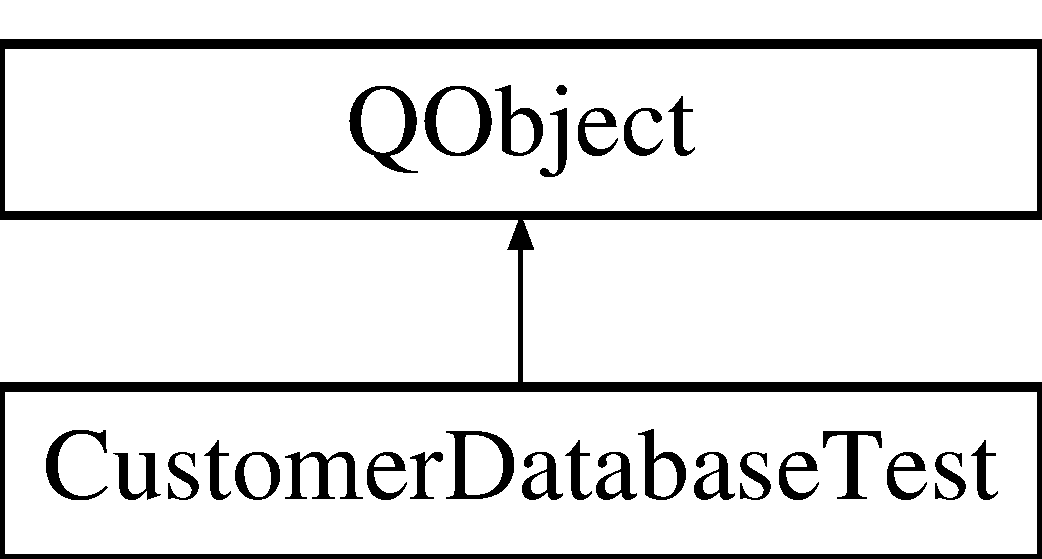
\includegraphics[height=2.000000cm]{d2/d63/classCustomerDatabaseTest}
\end{center}
\end{figure}


The documentation for this class was generated from the following files\-:\begin{DoxyCompactItemize}
\item 
/home/florent/\-Documents/\-Projet\-\_\-\-S8/\-Fact\-Dev/tests/database/customerdatabasetest.\-h\item 
/home/florent/\-Documents/\-Projet\-\_\-\-S8/\-Fact\-Dev/tests/database/customerdatabasetest.\-cpp\end{DoxyCompactItemize}

\hypertarget{classCustomerDataWidget}{\section{Customer\+Data\+Widget Class Reference}
\label{classCustomerDataWidget}\index{Customer\+Data\+Widget@{Customer\+Data\+Widget}}
}
Inheritance diagram for Customer\+Data\+Widget\+:\begin{figure}[H]
\begin{center}
\leavevmode
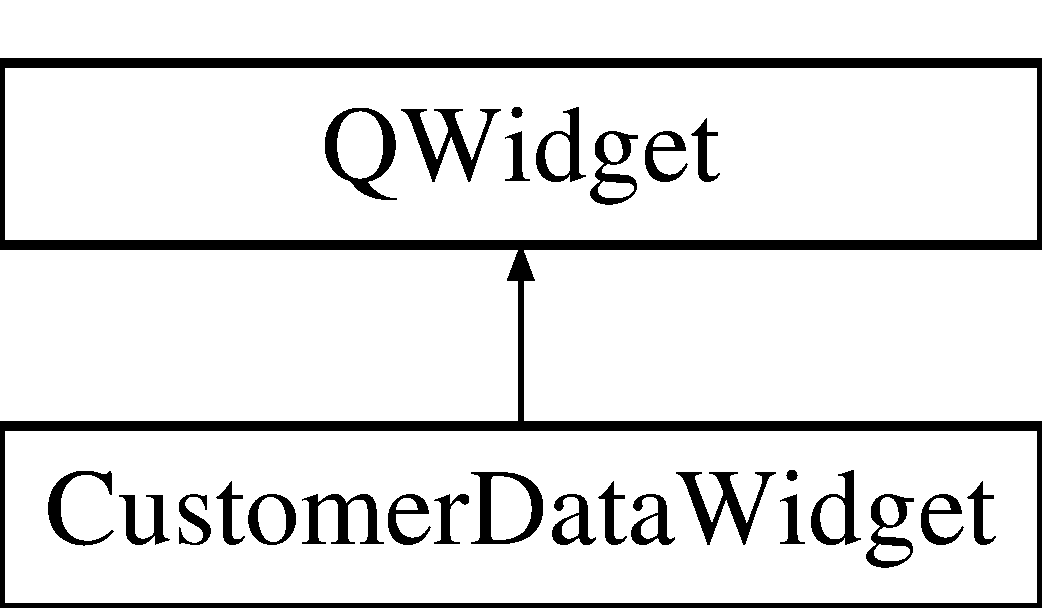
\includegraphics[height=2.000000cm]{df/df4/classCustomerDataWidget}
\end{center}
\end{figure}
\subsection*{Public Member Functions}
\begin{DoxyCompactItemize}
\item 
\hypertarget{classCustomerDataWidget_ae629d9d3839bd9f067927b19e1bb85cd}{{\bfseries Customer\+Data\+Widget} (Q\+Widget $\ast$parent=0)}\label{classCustomerDataWidget_ae629d9d3839bd9f067927b19e1bb85cd}

\item 
\hypertarget{classCustomerDataWidget_a9a56bd1d7faf76d083cfa97f2883bdf1}{void {\bfseries print\+User\+Data} ()}\label{classCustomerDataWidget_a9a56bd1d7faf76d083cfa97f2883bdf1}

\item 
\hypertarget{classCustomerDataWidget_ab61052cc337e51d1e34149d67816c58f}{void {\bfseries print\+Informations} (int id)}\label{classCustomerDataWidget_ab61052cc337e51d1e34149d67816c58f}

\end{DoxyCompactItemize}


The documentation for this class was generated from the following files\+:\begin{DoxyCompactItemize}
\item 
src/widgets/customerdatawidget.\+h\item 
src/widgets/customerdatawidget.\+cpp\end{DoxyCompactItemize}

\hypertarget{classCustomerModelTest}{\section{Customer\-Model\-Test Class Reference}
\label{classCustomerModelTest}\index{Customer\-Model\-Test@{Customer\-Model\-Test}}
}
Inheritance diagram for Customer\-Model\-Test\-:\begin{figure}[H]
\begin{center}
\leavevmode
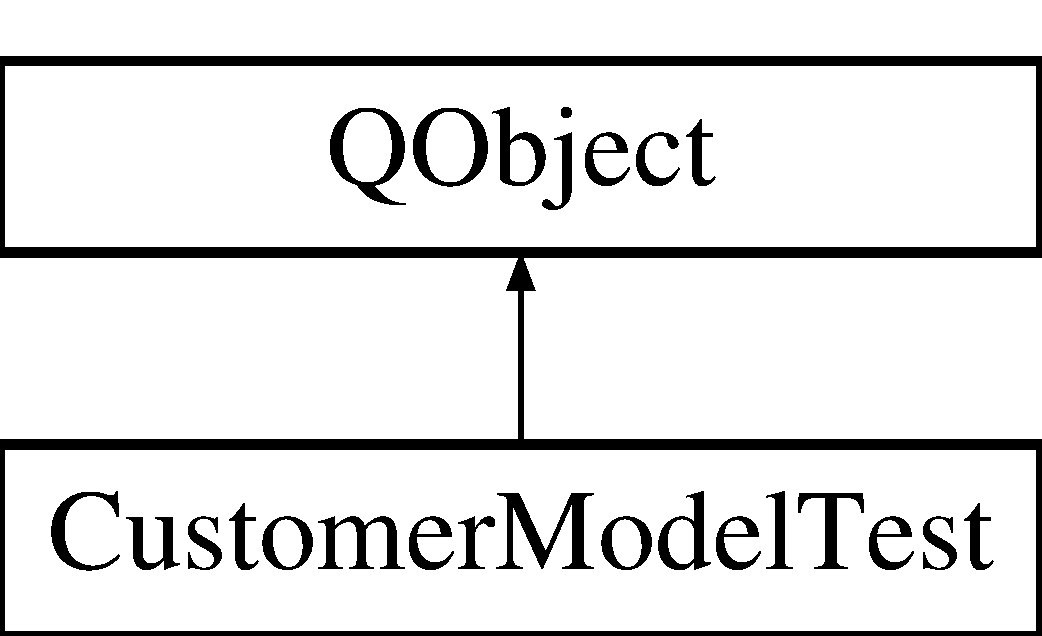
\includegraphics[height=2.000000cm]{d5/dcd/classCustomerModelTest}
\end{center}
\end{figure}


The documentation for this class was generated from the following files\-:\begin{DoxyCompactItemize}
\item 
/home/travis/build/\-F\-A\-C\-T-\/\-Team/\-Fact\-Dev/tests/models/customermodeltest.\-h\item 
/home/travis/build/\-F\-A\-C\-T-\/\-Team/\-Fact\-Dev/tests/models/customermodeltest.\-cpp\end{DoxyCompactItemize}

\hypertarget{classDatabase}{\section{Database Class Reference}
\label{classDatabase}\index{Database@{Database}}
}


The {\bfseries \hyperlink{classDatabase}{Database}} class Master class for all database access.  




{\ttfamily \#include $<$database.\-h$>$}

Inheritance diagram for Database\-:\begin{figure}[H]
\begin{center}
\leavevmode
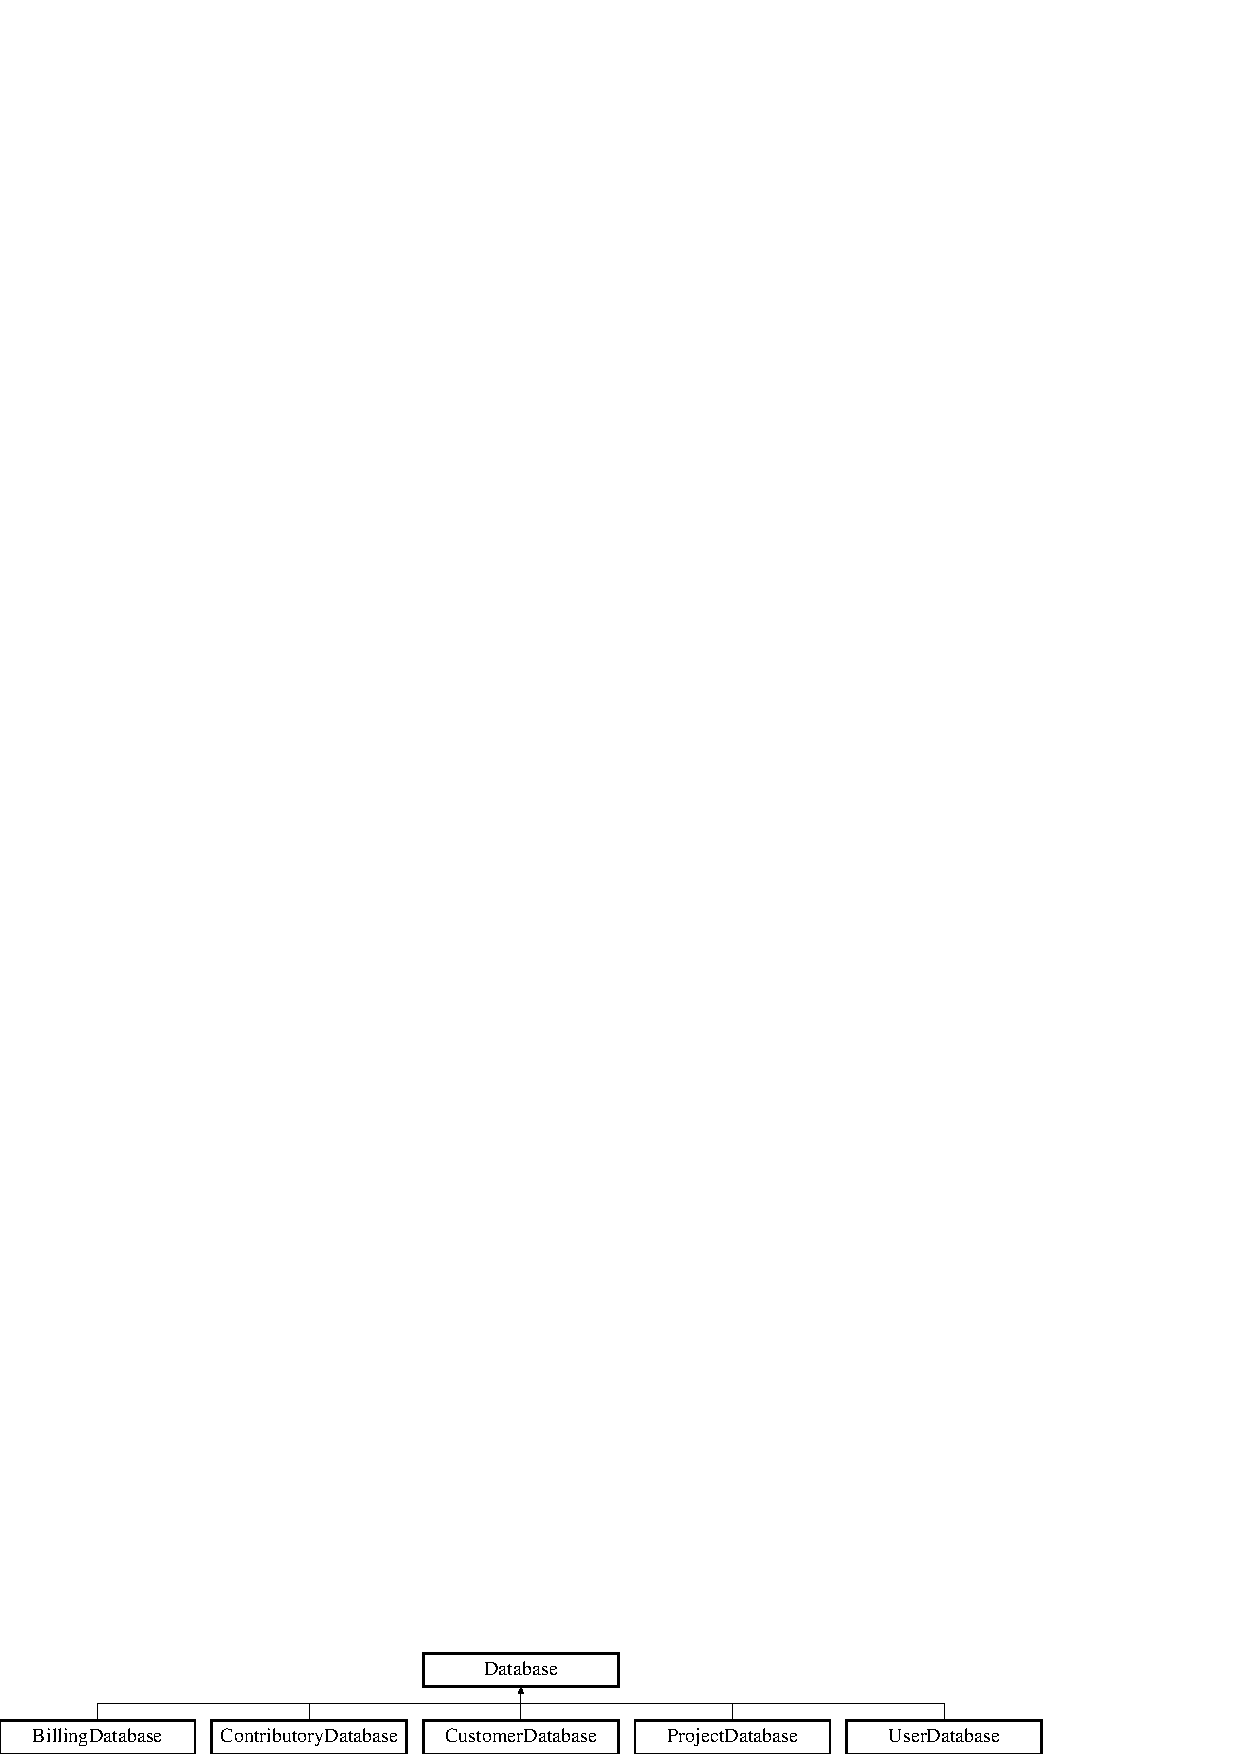
\includegraphics[height=2.000000cm]{de/d03/classDatabase}
\end{center}
\end{figure}
\subsection*{Public Member Functions}
\begin{DoxyCompactItemize}
\item 
Q\-String \hyperlink{classDatabase_a17465cc3fe0a8b853f96599e0584cc84}{last\-Error} (const Q\-Sql\-Query \&q)
\begin{DoxyCompactList}\small\item\em \hyperlink{classDatabase_a17465cc3fe0a8b853f96599e0584cc84}{Database\-::last\-Error} Return an error message on the last error occured during the S\-Q\-L request {\itshape q} \end{DoxyCompactList}\item 
void \hyperlink{classDatabase_a702ce00658c10518d2ddbbd234a0c67d}{test\-Cases} ()
\begin{DoxyCompactList}\small\item\em \hyperlink{classDatabase_a702ce00658c10518d2ddbbd234a0c67d}{Database\-::test\-Cases} Realise a test cases. \end{DoxyCompactList}\item 
\hypertarget{classDatabase_a6c7ca19f0107fdad000c268fc2b14ac0}{void \hyperlink{classDatabase_a6c7ca19f0107fdad000c268fc2b14ac0}{clean\-Database} ()}\label{classDatabase_a6c7ca19f0107fdad000c268fc2b14ac0}

\begin{DoxyCompactList}\small\item\em Database\-::vider\-Database Clear database. \end{DoxyCompactList}\item 
void \hyperlink{classDatabase_a06216acb010c0ea93ac2a53aa46256c2}{execute\-File} (Q\-String p\-Name)
\begin{DoxyCompactList}\small\item\em Database\-::executer\-Fichier Exeute a specified file named {\itshape p\-Name} \end{DoxyCompactList}\item 
\hypertarget{classDatabase_ace56e75784477e79197485e9b5980804}{void \hyperlink{classDatabase_ace56e75784477e79197485e9b5980804}{open\-Transaction} ()}\label{classDatabase_ace56e75784477e79197485e9b5980804}

\begin{DoxyCompactList}\small\item\em \hyperlink{classDatabase_ace56e75784477e79197485e9b5980804}{Database\-::open\-Transaction} Open new transaction. \end{DoxyCompactList}\item 
\hypertarget{classDatabase_a8322990bcba006d0d82ac069ad6e0307}{void \hyperlink{classDatabase_a8322990bcba006d0d82ac069ad6e0307}{close\-Transaction} ()}\label{classDatabase_a8322990bcba006d0d82ac069ad6e0307}

\begin{DoxyCompactList}\small\item\em \hyperlink{classDatabase_a8322990bcba006d0d82ac069ad6e0307}{Database\-::close\-Transaction} Close current transaction. \end{DoxyCompactList}\item 
\hypertarget{classDatabase_ab89cb07242f0ab1d4058974bf3e7cf19}{void \hyperlink{classDatabase_ab89cb07242f0ab1d4058974bf3e7cf19}{close} ()}\label{classDatabase_ab89cb07242f0ab1d4058974bf3e7cf19}

\begin{DoxyCompactList}\small\item\em \hyperlink{classDatabase_ab89cb07242f0ab1d4058974bf3e7cf19}{Database\-::close} Close database access. \end{DoxyCompactList}\item 
\hypertarget{classDatabase_a0d0134e05c8f2dc4fcbbb2f36c02a779}{void \hyperlink{classDatabase_a0d0134e05c8f2dc4fcbbb2f36c02a779}{open} ()}\label{classDatabase_a0d0134e05c8f2dc4fcbbb2f36c02a779}

\begin{DoxyCompactList}\small\item\em \hyperlink{classDatabase_a0d0134e05c8f2dc4fcbbb2f36c02a779}{Database\-::open} Open database. \end{DoxyCompactList}\item 
\hypertarget{classDatabase_a84d399a2ad58d69daab9b05330e1316d}{\hyperlink{classDatabase_a84d399a2ad58d69daab9b05330e1316d}{$\sim$\-Database} ()}\label{classDatabase_a84d399a2ad58d69daab9b05330e1316d}

\begin{DoxyCompactList}\small\item\em \hyperlink{classDatabase_a84d399a2ad58d69daab9b05330e1316d}{Database\-::$\sim$\-Database} Suppression object, and close database access. \end{DoxyCompactList}\item 
void \hyperlink{classDatabase_a8b03d7f4a92325b9e519fd3f8a2e245c}{set\-Database} (Q\-Sql\-Database sql)
\begin{DoxyCompactList}\small\item\em \hyperlink{classDatabase_a8b03d7f4a92325b9e519fd3f8a2e245c}{Database\-::set\-Database} Set database. \end{DoxyCompactList}\item 
\hypertarget{classDatabase_a2dc260583a49889bed8097e21953594e}{void \hyperlink{classDatabase_a2dc260583a49889bed8097e21953594e}{create\-Database} ()}\label{classDatabase_a2dc260583a49889bed8097e21953594e}

\begin{DoxyCompactList}\small\item\em Database\-::creer\-Database Create a new database. \end{DoxyCompactList}\end{DoxyCompactItemize}
\subsection*{Static Public Member Functions}
\begin{DoxyCompactItemize}
\item 
static \hyperlink{classDatabase}{Database} $\ast$ \hyperlink{classDatabase_aa334760d1e18f82a344fb696547bfa5c}{instance} ()  throw (\-Db\-Exception$\ast$)
\begin{DoxyCompactList}\small\item\em Database\-::get\-Instance Return an instance of \hyperlink{classDatabase}{Database}. \end{DoxyCompactList}\end{DoxyCompactItemize}
\subsection*{Protected Member Functions}
\begin{DoxyCompactItemize}
\item 
\hypertarget{classDatabase_a4703c80e6969d33565ea340f768fdadf}{\hyperlink{classDatabase_a4703c80e6969d33565ea340f768fdadf}{Database} ()  throw (\-Db\-Exception$\ast$)}\label{classDatabase_a4703c80e6969d33565ea340f768fdadf}

\begin{DoxyCompactList}\small\item\em \hyperlink{classDatabase_a4703c80e6969d33565ea340f768fdadf}{Database\-::\-Database} \hyperlink{classDatabase}{Database} is a singleton. \end{DoxyCompactList}\item 
Q\-Variant \hyperlink{classDatabase_a88f0ccd102fc421fb10ddad0fd94e8c1}{value} (const Q\-Sql\-Query \&q, const Q\-String \&champ)
\begin{DoxyCompactList}\small\item\em Database\-::valeur Value of database field. \end{DoxyCompactList}\end{DoxyCompactItemize}
\subsection*{Protected Attributes}
\begin{DoxyCompactItemize}
\item 
\hypertarget{classDatabase_a6cde413cb6d644c835406c09ec37947e}{Q\-Settings $\ast$ {\bfseries \-\_\-settings}}\label{classDatabase_a6cde413cb6d644c835406c09ec37947e}

\item 
\hypertarget{classDatabase_a64b9dbb3a5e6f42447a24caf726782e1}{Q\-Sql\-Database {\bfseries m\-Database}}\label{classDatabase_a64b9dbb3a5e6f42447a24caf726782e1}

\item 
\hypertarget{classDatabase_a9202583fae82c7f4ecbda6cb11b978c8}{Q\-List$<$ \hyperlink{classDatabase}{Database} $\ast$ $>$ {\bfseries \-\_\-instances}}\label{classDatabase_a9202583fae82c7f4ecbda6cb11b978c8}

\end{DoxyCompactItemize}
\subsection*{Static Protected Attributes}
\begin{DoxyCompactItemize}
\item 
\hypertarget{classDatabase_a4f435119a26cf1b0b8cca652a74c70b7}{static \hyperlink{classDatabase}{Database} $\ast$ {\bfseries \-\_\-instance} = 0}\label{classDatabase_a4f435119a26cf1b0b8cca652a74c70b7}

\item 
\hypertarget{classDatabase_a923366369d404e62e9e77111d7c21bab}{static bool {\bfseries \-\_\-db\-Instance} = 0}\label{classDatabase_a923366369d404e62e9e77111d7c21bab}

\item 
\hypertarget{classDatabase_a8ed9b8afac7134aa48e40c48780b240f}{static bool {\bfseries is\-Open} = false}\label{classDatabase_a8ed9b8afac7134aa48e40c48780b240f}

\end{DoxyCompactItemize}


\subsection{Detailed Description}
The {\bfseries \hyperlink{classDatabase}{Database}} class Master class for all database access. 

\begin{DoxyAuthor}{Author}
Antoine de Roquemaurel 
\end{DoxyAuthor}


\subsection{Member Function Documentation}
\hypertarget{classDatabase_a06216acb010c0ea93ac2a53aa46256c2}{\index{Database@{Database}!execute\-File@{execute\-File}}
\index{execute\-File@{execute\-File}!Database@{Database}}
\subsubsection[{execute\-File}]{\setlength{\rightskip}{0pt plus 5cm}void Database\-::execute\-File (
\begin{DoxyParamCaption}
\item[{Q\-String}]{p\-Name}
\end{DoxyParamCaption}
)}}\label{classDatabase_a06216acb010c0ea93ac2a53aa46256c2}


Database\-::executer\-Fichier Exeute a specified file named {\itshape p\-Name} 

Database\-::executer\-Fichier Exeute a specified file.


\begin{DoxyParams}{Parameters}
{\em p\-Nom} & File name \\
\hline
\end{DoxyParams}
\hypertarget{classDatabase_aa334760d1e18f82a344fb696547bfa5c}{\index{Database@{Database}!instance@{instance}}
\index{instance@{instance}!Database@{Database}}
\subsubsection[{instance}]{\setlength{\rightskip}{0pt plus 5cm}{\bf Database} $\ast$ Database\-::instance (
\begin{DoxyParamCaption}
{}
\end{DoxyParamCaption}
) throw  {\bf Db\-Exception} $\ast$) \hspace{0.3cm}{\ttfamily [static]}}}\label{classDatabase_aa334760d1e18f82a344fb696547bfa5c}


Database\-::get\-Instance Return an instance of \hyperlink{classDatabase}{Database}. 

\begin{DoxyReturn}{Returns}
Instance of \hyperlink{classDatabase}{Database} 
\end{DoxyReturn}
\hypertarget{classDatabase_a17465cc3fe0a8b853f96599e0584cc84}{\index{Database@{Database}!last\-Error@{last\-Error}}
\index{last\-Error@{last\-Error}!Database@{Database}}
\subsubsection[{last\-Error}]{\setlength{\rightskip}{0pt plus 5cm}Q\-String Database\-::last\-Error (
\begin{DoxyParamCaption}
\item[{const Q\-Sql\-Query \&}]{q}
\end{DoxyParamCaption}
)\hspace{0.3cm}{\ttfamily [inline]}}}\label{classDatabase_a17465cc3fe0a8b853f96599e0584cc84}


\hyperlink{classDatabase_a17465cc3fe0a8b853f96599e0584cc84}{Database\-::last\-Error} Return an error message on the last error occured during the S\-Q\-L request {\itshape q} 

Database\-::derniere\-Erreur Return text of last error.


\begin{DoxyParams}{Parameters}
{\em q} & S\-Q\-L request \\
\hline
\end{DoxyParams}
\begin{DoxyReturn}{Returns}
an error message
\end{DoxyReturn}

\begin{DoxyParams}{Parameters}
{\em q} & Query \\
\hline
\end{DoxyParams}
\begin{DoxyReturn}{Returns}
error message 
\end{DoxyReturn}
\hypertarget{classDatabase_a8b03d7f4a92325b9e519fd3f8a2e245c}{\index{Database@{Database}!set\-Database@{set\-Database}}
\index{set\-Database@{set\-Database}!Database@{Database}}
\subsubsection[{set\-Database}]{\setlength{\rightskip}{0pt plus 5cm}void Database\-::set\-Database (
\begin{DoxyParamCaption}
\item[{Q\-Sql\-Database}]{sql}
\end{DoxyParamCaption}
)}}\label{classDatabase_a8b03d7f4a92325b9e519fd3f8a2e245c}


\hyperlink{classDatabase_a8b03d7f4a92325b9e519fd3f8a2e245c}{Database\-::set\-Database} Set database. 


\begin{DoxyParams}{Parameters}
{\em sql} & The new database \\
\hline
\end{DoxyParams}
\hypertarget{classDatabase_a702ce00658c10518d2ddbbd234a0c67d}{\index{Database@{Database}!test\-Cases@{test\-Cases}}
\index{test\-Cases@{test\-Cases}!Database@{Database}}
\subsubsection[{test\-Cases}]{\setlength{\rightskip}{0pt plus 5cm}void Database\-::test\-Cases (
\begin{DoxyParamCaption}
{}
\end{DoxyParamCaption}
)\hspace{0.3cm}{\ttfamily [inline]}}}\label{classDatabase_a702ce00658c10518d2ddbbd234a0c67d}


\hyperlink{classDatabase_a702ce00658c10518d2ddbbd234a0c67d}{Database\-::test\-Cases} Realise a test cases. 

Database\-::jeu\-D\-Essai Create. \hypertarget{classDatabase_a88f0ccd102fc421fb10ddad0fd94e8c1}{\index{Database@{Database}!value@{value}}
\index{value@{value}!Database@{Database}}
\subsubsection[{value}]{\setlength{\rightskip}{0pt plus 5cm}Q\-Variant Database\-::value (
\begin{DoxyParamCaption}
\item[{const Q\-Sql\-Query \&}]{q, }
\item[{const Q\-String \&}]{champ}
\end{DoxyParamCaption}
)\hspace{0.3cm}{\ttfamily [protected]}}}\label{classDatabase_a88f0ccd102fc421fb10ddad0fd94e8c1}


Database\-::valeur Value of database field. 


\begin{DoxyParams}{Parameters}
{\em q} & Query \\
\hline
{\em champ} & Field \\
\hline
\end{DoxyParams}
\begin{DoxyReturn}{Returns}
The value 
\end{DoxyReturn}


The documentation for this class was generated from the following files\-:\begin{DoxyCompactItemize}
\item 
/home/florent/\-Documents/\-Projet\-\_\-\-S8/\-Fact\-Dev/src/database/database.\-h\item 
/home/florent/\-Documents/\-Projet\-\_\-\-S8/\-Fact\-Dev/src/database/database.\-cpp\end{DoxyCompactItemize}

\hypertarget{classDbException}{\section{Db\+Exception Class Reference}
\label{classDbException}\index{Db\+Exception@{Db\+Exception}}
}


The \hyperlink{classDbException}{Db\+Exception} class for database exception \+: queries, db file, …  




{\ttfamily \#include $<$dbexception.\+h$>$}

Inheritance diagram for Db\+Exception\+:\begin{figure}[H]
\begin{center}
\leavevmode
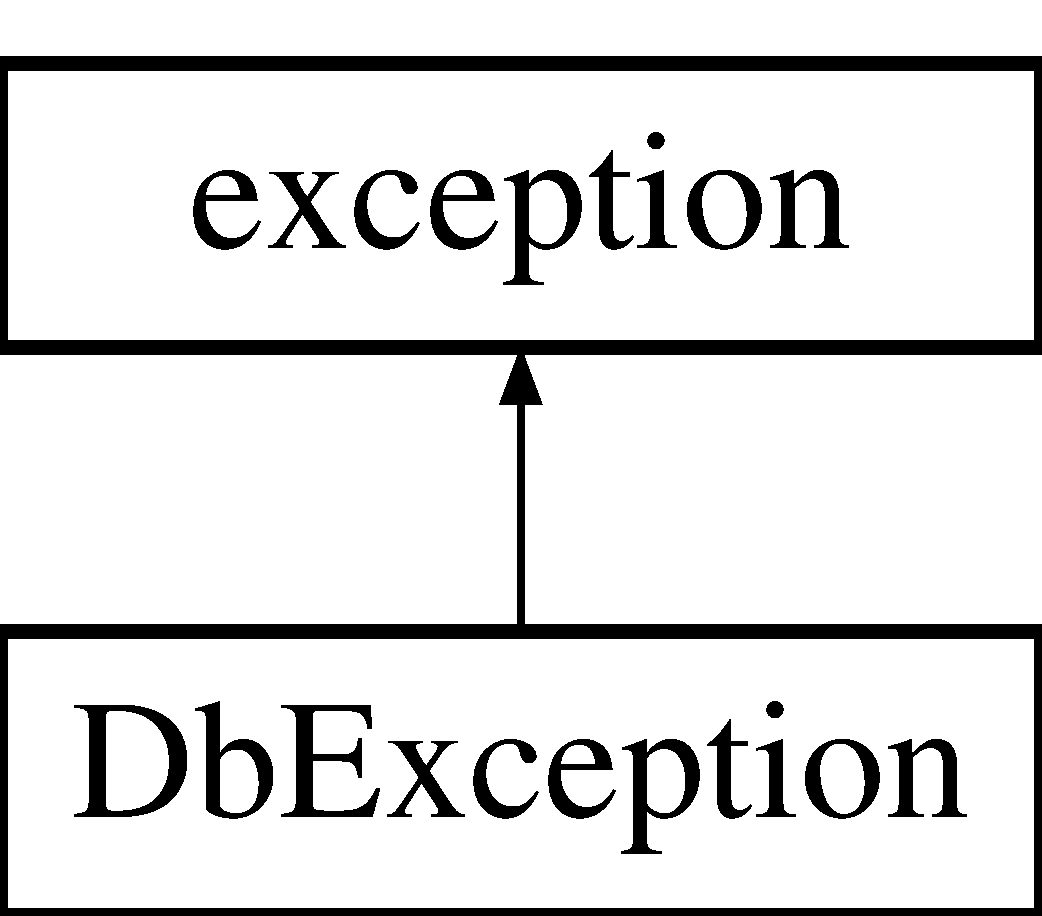
\includegraphics[height=2.000000cm]{dd/dca/classDbException}
\end{center}
\end{figure}
\subsection*{Public Member Functions}
\begin{DoxyCompactItemize}
\item 
\hyperlink{classDbException_a22204317679895d999e3621cf97d5dee}{Db\+Exception} (const Q\+String fct, const Q\+String fct\+Name, const Q\+String log\+Error, float error\+Code)
\begin{DoxyCompactList}\small\item\em \hyperlink{classDbException_a22204317679895d999e3621cf97d5dee}{Db\+Exception\+::\+Db\+Exception}. Construct a \hyperlink{classDbException}{Db\+Exception}. \end{DoxyCompactList}\item 
\hypertarget{classDbException_a57b57d4d9010c06d158ccc44d45a1376}{virtual \hyperlink{classDbException_a57b57d4d9010c06d158ccc44d45a1376}{$\sim$\+Db\+Exception} ()  throw ()}\label{classDbException_a57b57d4d9010c06d158ccc44d45a1376}

\begin{DoxyCompactList}\small\item\em $\sim$\+Db\+Exception \end{DoxyCompactList}\item 
void \hyperlink{classDbException_a06765391cd11f596721c877c1a62c2f1}{popup\+Message} (Q\+Widget $\ast$parent)
\begin{DoxyCompactList}\small\item\em \hyperlink{classDbException_a06765391cd11f596721c877c1a62c2f1}{Db\+Exception\+::popup\+Message}. Display a popup message with the message error. \end{DoxyCompactList}\end{DoxyCompactItemize}


\subsection{Detailed Description}
The \hyperlink{classDbException}{Db\+Exception} class for database exception \+: queries, db file, … 

\begin{DoxyAuthor}{Author}
Antoine de Roquemaurel 
\end{DoxyAuthor}


\subsection{Constructor \& Destructor Documentation}
\hypertarget{classDbException_a22204317679895d999e3621cf97d5dee}{\index{Db\+Exception@{Db\+Exception}!Db\+Exception@{Db\+Exception}}
\index{Db\+Exception@{Db\+Exception}!Db\+Exception@{Db\+Exception}}
\subsubsection[{Db\+Exception}]{\setlength{\rightskip}{0pt plus 5cm}Db\+Exception\+::\+Db\+Exception (
\begin{DoxyParamCaption}
\item[{const Q\+String}]{fct, }
\item[{const Q\+String}]{fct\+Name, }
\item[{const Q\+String}]{log\+Error, }
\item[{float}]{error\+Code}
\end{DoxyParamCaption}
)}}\label{classDbException_a22204317679895d999e3621cf97d5dee}


\hyperlink{classDbException_a22204317679895d999e3621cf97d5dee}{Db\+Exception\+::\+Db\+Exception}. Construct a \hyperlink{classDbException}{Db\+Exception}. 


\begin{DoxyParams}{Parameters}
{\em user\+Error} & Class\+Name of error \\
\hline
{\em fct\+Name} & Function name \\
\hline
{\em log\+Error} & Message error \\
\hline
{\em error\+Code} & Code of error \\
\hline
\end{DoxyParams}


\subsection{Member Function Documentation}
\hypertarget{classDbException_a06765391cd11f596721c877c1a62c2f1}{\index{Db\+Exception@{Db\+Exception}!popup\+Message@{popup\+Message}}
\index{popup\+Message@{popup\+Message}!Db\+Exception@{Db\+Exception}}
\subsubsection[{popup\+Message}]{\setlength{\rightskip}{0pt plus 5cm}void Db\+Exception\+::popup\+Message (
\begin{DoxyParamCaption}
\item[{Q\+Widget $\ast$}]{parent}
\end{DoxyParamCaption}
)}}\label{classDbException_a06765391cd11f596721c877c1a62c2f1}


\hyperlink{classDbException_a06765391cd11f596721c877c1a62c2f1}{Db\+Exception\+::popup\+Message}. Display a popup message with the message error. 


\begin{DoxyParams}{Parameters}
{\em parent} & \\
\hline
\end{DoxyParams}


The documentation for this class was generated from the following files\+:\begin{DoxyCompactItemize}
\item 
src/exceptions/dbexception.\+h\item 
src/exceptions/dbexception.\+cpp\end{DoxyCompactItemize}

\hypertarget{classDialogAddCustomer}{\section{Dialog\+Add\+Customer Class Reference}
\label{classDialogAddCustomer}\index{Dialog\+Add\+Customer@{Dialog\+Add\+Customer}}
}


The \hyperlink{classDialogAddCustomer}{Dialog\+Add\+Customer} class Window to add or modify a \hyperlink{classCustomer}{Customer}.  




{\ttfamily \#include $<$dialogaddcustomer.\+h$>$}

Inheritance diagram for Dialog\+Add\+Customer\+:\begin{figure}[H]
\begin{center}
\leavevmode
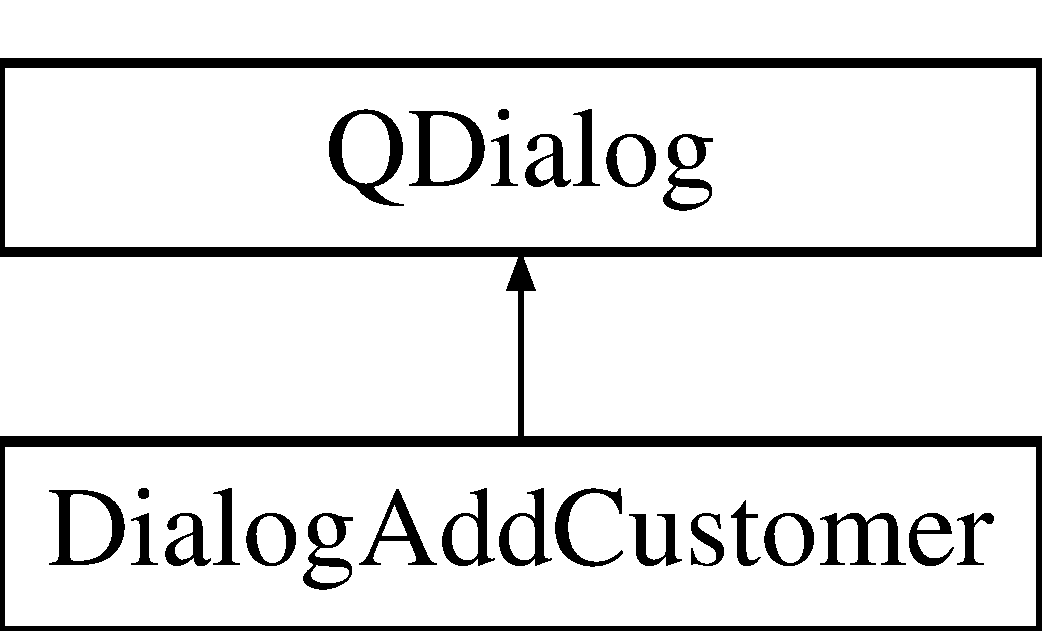
\includegraphics[height=2.000000cm]{df/d01/classDialogAddCustomer}
\end{center}
\end{figure}
\subsection*{Public Member Functions}
\begin{DoxyCompactItemize}
\item 
\hyperlink{classDialogAddCustomer_a6123adb32813c5ebe71ce06012c46b9c}{Dialog\+Add\+Customer} (int id=0, Q\+Widget $\ast$parent=0)
\begin{DoxyCompactList}\small\item\em \hyperlink{classDialogAddCustomer}{Dialog\+Add\+Customer} Construct a window to add/modify a \hyperlink{classCustomer}{Customer}. \end{DoxyCompactList}\item 
\hypertarget{classDialogAddCustomer_ae06c708abccad5ce0b8523c94b40eb75}{void \hyperlink{classDialogAddCustomer_ae06c708abccad5ce0b8523c94b40eb75}{fill\+Fields} ()}\label{classDialogAddCustomer_ae06c708abccad5ce0b8523c94b40eb75}

\begin{DoxyCompactList}\small\item\em fill\+Fields If the \hyperlink{classCustomer}{Customer} exits, fill line edits with the data of the current \hyperlink{classCustomer}{Customer} \end{DoxyCompactList}\item 
\hypertarget{classDialogAddCustomer_a1492352d114740bb44178f2415555155}{void \hyperlink{classDialogAddCustomer_a1492352d114740bb44178f2415555155}{accept} ()}\label{classDialogAddCustomer_a1492352d114740bb44178f2415555155}

\begin{DoxyCompactList}\small\item\em accept Valid data inputed by user and add these data in \hyperlink{classDatabase}{Database} \end{DoxyCompactList}\item 
\hypertarget{classDialogAddCustomer_a6affc8db156ee183ffd14a71d06a8534}{void \hyperlink{classDialogAddCustomer_a6affc8db156ee183ffd14a71d06a8534}{reject} ()}\label{classDialogAddCustomer_a6affc8db156ee183ffd14a71d06a8534}

\begin{DoxyCompactList}\small\item\em reject Cancel the operation and close the windows \end{DoxyCompactList}\item 
\hypertarget{classDialogAddCustomer_a65516413d3d3cb78acb03f5b45bc0278}{\hyperlink{classCustomer}{Customer} $\ast$ {\bfseries get\+Custom} () const }\label{classDialogAddCustomer_a65516413d3d3cb78acb03f5b45bc0278}

\item 
\hypertarget{classDialogAddCustomer_afde6fa7e1b2758d56f400fd719dfb603}{void {\bfseries set\+Custom} (\hyperlink{classCustomer}{Customer} $\ast$get\+Custom)}\label{classDialogAddCustomer_afde6fa7e1b2758d56f400fd719dfb603}

\end{DoxyCompactItemize}


\subsection{Detailed Description}
The \hyperlink{classDialogAddCustomer}{Dialog\+Add\+Customer} class Window to add or modify a \hyperlink{classCustomer}{Customer}. 

\begin{DoxyAuthor}{Author}
Cédric Rohaut 
\end{DoxyAuthor}


\subsection{Constructor \& Destructor Documentation}
\hypertarget{classDialogAddCustomer_a6123adb32813c5ebe71ce06012c46b9c}{\index{Dialog\+Add\+Customer@{Dialog\+Add\+Customer}!Dialog\+Add\+Customer@{Dialog\+Add\+Customer}}
\index{Dialog\+Add\+Customer@{Dialog\+Add\+Customer}!Dialog\+Add\+Customer@{Dialog\+Add\+Customer}}
\subsubsection[{Dialog\+Add\+Customer}]{\setlength{\rightskip}{0pt plus 5cm}Dialog\+Add\+Customer\+::\+Dialog\+Add\+Customer (
\begin{DoxyParamCaption}
\item[{int}]{id = {\ttfamily 0}, }
\item[{Q\+Widget $\ast$}]{parent = {\ttfamily 0}}
\end{DoxyParamCaption}
)\hspace{0.3cm}{\ttfamily [explicit]}}}\label{classDialogAddCustomer_a6123adb32813c5ebe71ce06012c46b9c}


\hyperlink{classDialogAddCustomer}{Dialog\+Add\+Customer} Construct a window to add/modify a \hyperlink{classCustomer}{Customer}. 


\begin{DoxyParams}{Parameters}
{\em id} & \hyperlink{classCustomer}{Customer} id \\
\hline
{\em parent} & Q\+Widget parent \\
\hline
\end{DoxyParams}


The documentation for this class was generated from the following files\+:\begin{DoxyCompactItemize}
\item 
src/dialogs/dialogaddcustomer.\+h\item 
src/dialogs/dialogaddcustomer.\+cpp\end{DoxyCompactItemize}

\hypertarget{classIDatabaseModel}{\section{I\+Database\+Model Class Reference}
\label{classIDatabaseModel}\index{I\+Database\+Model@{I\+Database\+Model}}
}


The \hyperlink{classIDatabaseModel}{I\+Database\+Model} class.  




{\ttfamily \#include $<$idatabasemodel.\+h$>$}

Inheritance diagram for I\+Database\+Model\+:\begin{figure}[H]
\begin{center}
\leavevmode
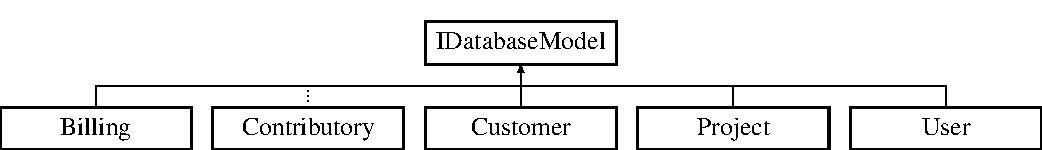
\includegraphics[height=2.000000cm]{d1/dc3/classIDatabaseModel}
\end{center}
\end{figure}
\subsection*{Public Member Functions}
\begin{DoxyCompactItemize}
\item 
\hypertarget{classIDatabaseModel_a85b66486922fe56a18c897cf93ed33a2}{virtual \hyperlink{classIDatabaseModel_a85b66486922fe56a18c897cf93ed33a2}{$\sim$\+I\+Database\+Model} ()}\label{classIDatabaseModel_a85b66486922fe56a18c897cf93ed33a2}

\begin{DoxyCompactList}\small\item\em $\sim$\+I\+Database\+Model Remove an instance of \hyperlink{classIDatabaseModel}{I\+Database\+Model} \end{DoxyCompactList}\item 
\hypertarget{classIDatabaseModel_a2d4fd70557c1815d100df17ba0751cbd}{virtual void \hyperlink{classIDatabaseModel_a2d4fd70557c1815d100df17ba0751cbd}{commit} ()=0}\label{classIDatabaseModel_a2d4fd70557c1815d100df17ba0751cbd}

\begin{DoxyCompactList}\small\item\em \hyperlink{classIDatabaseModel_a2d4fd70557c1815d100df17ba0751cbd}{I\+Database\+Model\+::commit} Update or insert data into the database. \end{DoxyCompactList}\item 
virtual void \hyperlink{classIDatabaseModel_a25e44ed10a75976f86e14d34aea02c37}{hydrat} (int id)=0
\begin{DoxyCompactList}\small\item\em \hyperlink{classIDatabaseModel_a25e44ed10a75976f86e14d34aea02c37}{I\+Database\+Model\+::hydrat} Get data of the element which is specified by the identify {\itshape id} from the database. \end{DoxyCompactList}\item 
\hypertarget{classIDatabaseModel_a11d94697daf0af2b44fbe37ef831ea94}{virtual void \hyperlink{classIDatabaseModel_a11d94697daf0af2b44fbe37ef831ea94}{remove} ()=0}\label{classIDatabaseModel_a11d94697daf0af2b44fbe37ef831ea94}

\begin{DoxyCompactList}\small\item\em \hyperlink{classIDatabaseModel_a11d94697daf0af2b44fbe37ef831ea94}{I\+Database\+Model\+::remove} Remove the current element in the database. \end{DoxyCompactList}\item 
int \hyperlink{classIDatabaseModel_a61523b015ec148d4e68ee8054c2ad3e3}{get\+Id} () const 
\begin{DoxyCompactList}\small\item\em \hyperlink{classIDatabaseModel_a61523b015ec148d4e68ee8054c2ad3e3}{I\+Database\+Model\+::get\+Id} Return the identify of the element of the database. \end{DoxyCompactList}\item 
void \hyperlink{classIDatabaseModel_ad4f47f3e25302c506ce98103e616ca57}{set\+Id} (int id)
\begin{DoxyCompactList}\small\item\em \hyperlink{classIDatabaseModel_ad4f47f3e25302c506ce98103e616ca57}{I\+Database\+Model\+::set\+Id} Replace the current identify by {\itshape id} \end{DoxyCompactList}\item 
bool \hyperlink{classIDatabaseModel_a095166b2e37a0d07c4151a25ddbd89f9}{is\+To\+Removed} () const 
\begin{DoxyCompactList}\small\item\em to\+Removed return if object must be removed. \end{DoxyCompactList}\item 
void \hyperlink{classIDatabaseModel_a6c7d03b37e11a287dfe97a2e7bc12522}{set\+To\+Removed} (bool to\+Removed)
\begin{DoxyCompactList}\small\item\em set\+To\+Removed Change the flag for removed object \end{DoxyCompactList}\end{DoxyCompactItemize}
\subsection*{Protected Attributes}
\begin{DoxyCompactItemize}
\item 
\hypertarget{classIDatabaseModel_a49f0ca7727c7d12eb78f670c882a3028}{int \hyperlink{classIDatabaseModel_a49f0ca7727c7d12eb78f670c882a3028}{\+\_\+id}}\label{classIDatabaseModel_a49f0ca7727c7d12eb78f670c882a3028}

\begin{DoxyCompactList}\small\item\em Element identify. \end{DoxyCompactList}\item 
\hypertarget{classIDatabaseModel_a3353a9530b1b9e4af91c02a944b050ae}{bool \hyperlink{classIDatabaseModel_a3353a9530b1b9e4af91c02a944b050ae}{\+\_\+to\+Removed}}\label{classIDatabaseModel_a3353a9530b1b9e4af91c02a944b050ae}

\begin{DoxyCompactList}\small\item\em Flag to know if the object must be removed. \end{DoxyCompactList}\end{DoxyCompactItemize}


\subsection{Detailed Description}
The \hyperlink{classIDatabaseModel}{I\+Database\+Model} class. 

\begin{DoxyAuthor}{Author}
Antoine de Roquemaurel 
\end{DoxyAuthor}


\subsection{Member Function Documentation}
\hypertarget{classIDatabaseModel_a61523b015ec148d4e68ee8054c2ad3e3}{\index{I\+Database\+Model@{I\+Database\+Model}!get\+Id@{get\+Id}}
\index{get\+Id@{get\+Id}!I\+Database\+Model@{I\+Database\+Model}}
\subsubsection[{get\+Id}]{\setlength{\rightskip}{0pt plus 5cm}int I\+Database\+Model\+::get\+Id (
\begin{DoxyParamCaption}
{}
\end{DoxyParamCaption}
) const\hspace{0.3cm}{\ttfamily [inline]}}}\label{classIDatabaseModel_a61523b015ec148d4e68ee8054c2ad3e3}


\hyperlink{classIDatabaseModel_a61523b015ec148d4e68ee8054c2ad3e3}{I\+Database\+Model\+::get\+Id} Return the identify of the element of the database. 

\begin{DoxyReturn}{Returns}
identity 
\end{DoxyReturn}
\hypertarget{classIDatabaseModel_a25e44ed10a75976f86e14d34aea02c37}{\index{I\+Database\+Model@{I\+Database\+Model}!hydrat@{hydrat}}
\index{hydrat@{hydrat}!I\+Database\+Model@{I\+Database\+Model}}
\subsubsection[{hydrat}]{\setlength{\rightskip}{0pt plus 5cm}virtual void I\+Database\+Model\+::hydrat (
\begin{DoxyParamCaption}
\item[{int}]{id}
\end{DoxyParamCaption}
)\hspace{0.3cm}{\ttfamily [pure virtual]}}}\label{classIDatabaseModel_a25e44ed10a75976f86e14d34aea02c37}


\hyperlink{classIDatabaseModel_a25e44ed10a75976f86e14d34aea02c37}{I\+Database\+Model\+::hydrat} Get data of the element which is specified by the identify {\itshape id} from the database. 


\begin{DoxyParams}{Parameters}
{\em id} & \\
\hline
\end{DoxyParams}


Implemented in \hyperlink{classProject_aa966f15c9c8a277844a75c3530701525}{Project}, \hyperlink{classBilling_a8beb72061cd53a964cf0ba3f04686613}{Billing}, \hyperlink{classContributory_a2b834e0288c93ba9ed70acf7a0b8c32d}{Contributory}, \hyperlink{classUser_a2e4160755d2189979b758929e832b12c}{User}, and \hyperlink{classCustomer_ac77f54786ea2bd4c1696c0a76301c639}{Customer}.

\hypertarget{classIDatabaseModel_a095166b2e37a0d07c4151a25ddbd89f9}{\index{I\+Database\+Model@{I\+Database\+Model}!is\+To\+Removed@{is\+To\+Removed}}
\index{is\+To\+Removed@{is\+To\+Removed}!I\+Database\+Model@{I\+Database\+Model}}
\subsubsection[{is\+To\+Removed}]{\setlength{\rightskip}{0pt plus 5cm}bool I\+Database\+Model\+::is\+To\+Removed (
\begin{DoxyParamCaption}
{}
\end{DoxyParamCaption}
) const\hspace{0.3cm}{\ttfamily [inline]}}}\label{classIDatabaseModel_a095166b2e37a0d07c4151a25ddbd89f9}


to\+Removed return if object must be removed. 

\begin{DoxyReturn}{Returns}

\end{DoxyReturn}
\hypertarget{classIDatabaseModel_ad4f47f3e25302c506ce98103e616ca57}{\index{I\+Database\+Model@{I\+Database\+Model}!set\+Id@{set\+Id}}
\index{set\+Id@{set\+Id}!I\+Database\+Model@{I\+Database\+Model}}
\subsubsection[{set\+Id}]{\setlength{\rightskip}{0pt plus 5cm}void I\+Database\+Model\+::set\+Id (
\begin{DoxyParamCaption}
\item[{int}]{id}
\end{DoxyParamCaption}
)\hspace{0.3cm}{\ttfamily [inline]}}}\label{classIDatabaseModel_ad4f47f3e25302c506ce98103e616ca57}


\hyperlink{classIDatabaseModel_ad4f47f3e25302c506ce98103e616ca57}{I\+Database\+Model\+::set\+Id} Replace the current identify by {\itshape id} 


\begin{DoxyParams}{Parameters}
{\em id} & New identify \\
\hline
\end{DoxyParams}
\hypertarget{classIDatabaseModel_a6c7d03b37e11a287dfe97a2e7bc12522}{\index{I\+Database\+Model@{I\+Database\+Model}!set\+To\+Removed@{set\+To\+Removed}}
\index{set\+To\+Removed@{set\+To\+Removed}!I\+Database\+Model@{I\+Database\+Model}}
\subsubsection[{set\+To\+Removed}]{\setlength{\rightskip}{0pt plus 5cm}void I\+Database\+Model\+::set\+To\+Removed (
\begin{DoxyParamCaption}
\item[{bool}]{to\+Removed}
\end{DoxyParamCaption}
)\hspace{0.3cm}{\ttfamily [inline]}}}\label{classIDatabaseModel_a6c7d03b37e11a287dfe97a2e7bc12522}


set\+To\+Removed Change the flag for removed object 


\begin{DoxyParams}{Parameters}
{\em to\+Removed} & The new flag \\
\hline
\end{DoxyParams}


The documentation for this class was generated from the following file\+:\begin{DoxyCompactItemize}
\item 
src/models/idatabasemodel.\+h\end{DoxyCompactItemize}

\hypertarget{classLog}{\section{Log Class Reference}
\label{classLog}\index{Log@{Log}}
}


The \hyperlink{classLog}{Log} class for Simple management of log.  




{\ttfamily \#include $<$log.\-h$>$}

\subsection*{Public Member Functions}
\begin{DoxyCompactItemize}
\item 
\hypertarget{classLog_a0fbfda88fbee5027c89f6eb121059360}{\hyperlink{classLog_a0fbfda88fbee5027c89f6eb121059360}{$\sim$\-Log} ()}\label{classLog_a0fbfda88fbee5027c89f6eb121059360}

\begin{DoxyCompactList}\small\item\em \hyperlink{classLog_a0fbfda88fbee5027c89f6eb121059360}{Log\-::$\sim$\-Log}. \end{DoxyCompactList}\item 
void \hyperlink{classLog_acef079f691840d7afd2ed9482d5d66ea}{write} (const Q\-String text)
\begin{DoxyCompactList}\small\item\em \hyperlink{classLog_acef079f691840d7afd2ed9482d5d66ea}{Log\-::write}. Write log message in file. \end{DoxyCompactList}\item 
\hypertarget{classLog_af6071a60aa52b6c1b511f99b4bc1b8fe}{\hyperlink{classLog_af6071a60aa52b6c1b511f99b4bc1b8fe}{Log} ()}\label{classLog_af6071a60aa52b6c1b511f99b4bc1b8fe}

\begin{DoxyCompactList}\small\item\em \hyperlink{classLog_af6071a60aa52b6c1b511f99b4bc1b8fe}{Log\-::\-Log}. \hyperlink{classLog}{Log} is a singleton. \end{DoxyCompactList}\end{DoxyCompactItemize}
\subsection*{Static Public Member Functions}
\begin{DoxyCompactItemize}
\item 
static \hyperlink{classLog}{Log} \& \hyperlink{classLog_ad8ef93302c147f832ed8202a6b039eb5}{instance} (Type\-Log type=I\-N\-F\-O)
\begin{DoxyCompactList}\small\item\em \hyperlink{classLog_ad8ef93302c147f832ed8202a6b039eb5}{Log\-::instance}. Return the instance of logger. \end{DoxyCompactList}\end{DoxyCompactItemize}
\subsection*{Friends}
\begin{DoxyCompactItemize}
\item 
\hyperlink{classLog}{Log} \& \hyperlink{classLog_a1ecba3328cadecbbd7d65ae2852171fc}{operator$<$$<$} (\hyperlink{classLog}{Log} \&logger, const Q\-String \&text)
\begin{DoxyCompactList}\small\item\em operator $<$$<$ for log writing \end{DoxyCompactList}\end{DoxyCompactItemize}


\subsection{Detailed Description}
The \hyperlink{classLog}{Log} class for Simple management of log. 

\subsection{Member Function Documentation}
\hypertarget{classLog_ad8ef93302c147f832ed8202a6b039eb5}{\index{Log@{Log}!instance@{instance}}
\index{instance@{instance}!Log@{Log}}
\subsubsection[{instance}]{\setlength{\rightskip}{0pt plus 5cm}{\bf Log} \& Log\-::instance (
\begin{DoxyParamCaption}
\item[{Type\-Log}]{type = {\ttfamily INFO}}
\end{DoxyParamCaption}
)\hspace{0.3cm}{\ttfamily [static]}}}\label{classLog_ad8ef93302c147f832ed8202a6b039eb5}


\hyperlink{classLog_ad8ef93302c147f832ed8202a6b039eb5}{Log\-::instance}. Return the instance of logger. 


\begin{DoxyParams}{Parameters}
{\em type} & Type of log \-: W\-A\-R\-N\-I\-N\-G, I\-N\-F\-O, E\-R\-R\-O\-R \\
\hline
\end{DoxyParams}
\begin{DoxyReturn}{Returns}
Instance of logger. 
\end{DoxyReturn}
\hypertarget{classLog_acef079f691840d7afd2ed9482d5d66ea}{\index{Log@{Log}!write@{write}}
\index{write@{write}!Log@{Log}}
\subsubsection[{write}]{\setlength{\rightskip}{0pt plus 5cm}void Log\-::write (
\begin{DoxyParamCaption}
\item[{const Q\-String}]{text}
\end{DoxyParamCaption}
)}}\label{classLog_acef079f691840d7afd2ed9482d5d66ea}


\hyperlink{classLog_acef079f691840d7afd2ed9482d5d66ea}{Log\-::write}. Write log message in file. 


\begin{DoxyParams}{Parameters}
{\em text} & \\
\hline
\end{DoxyParams}


\subsection{Friends And Related Function Documentation}
\hypertarget{classLog_a1ecba3328cadecbbd7d65ae2852171fc}{\index{Log@{Log}!operator$<$$<$@{operator$<$$<$}}
\index{operator$<$$<$@{operator$<$$<$}!Log@{Log}}
\subsubsection[{operator$<$$<$}]{\setlength{\rightskip}{0pt plus 5cm}{\bf Log}\& operator$<$$<$ (
\begin{DoxyParamCaption}
\item[{{\bf Log} \&}]{logger, }
\item[{const Q\-String \&}]{text}
\end{DoxyParamCaption}
)\hspace{0.3cm}{\ttfamily [friend]}}}\label{classLog_a1ecba3328cadecbbd7d65ae2852171fc}


operator $<$$<$ for log writing 


\begin{DoxyParams}{Parameters}
{\em logger} & Instance of Logger \\
\hline
{\em text} & Text to write \\
\hline
\end{DoxyParams}
\begin{DoxyReturn}{Returns}
New logger. 
\end{DoxyReturn}


The documentation for this class was generated from the following files\-:\begin{DoxyCompactItemize}
\item 
/home/florent/\-Documents/\-Projet\-\_\-\-S8/\-Fact\-Dev/src/log.\-h\item 
/home/florent/\-Documents/\-Projet\-\_\-\-S8/\-Fact\-Dev/src/log.\-cpp\end{DoxyCompactItemize}

\hypertarget{classMainWindow}{\section{Main\-Window Class Reference}
\label{classMainWindow}\index{Main\-Window@{Main\-Window}}
}
Inheritance diagram for Main\-Window\-:\begin{figure}[H]
\begin{center}
\leavevmode
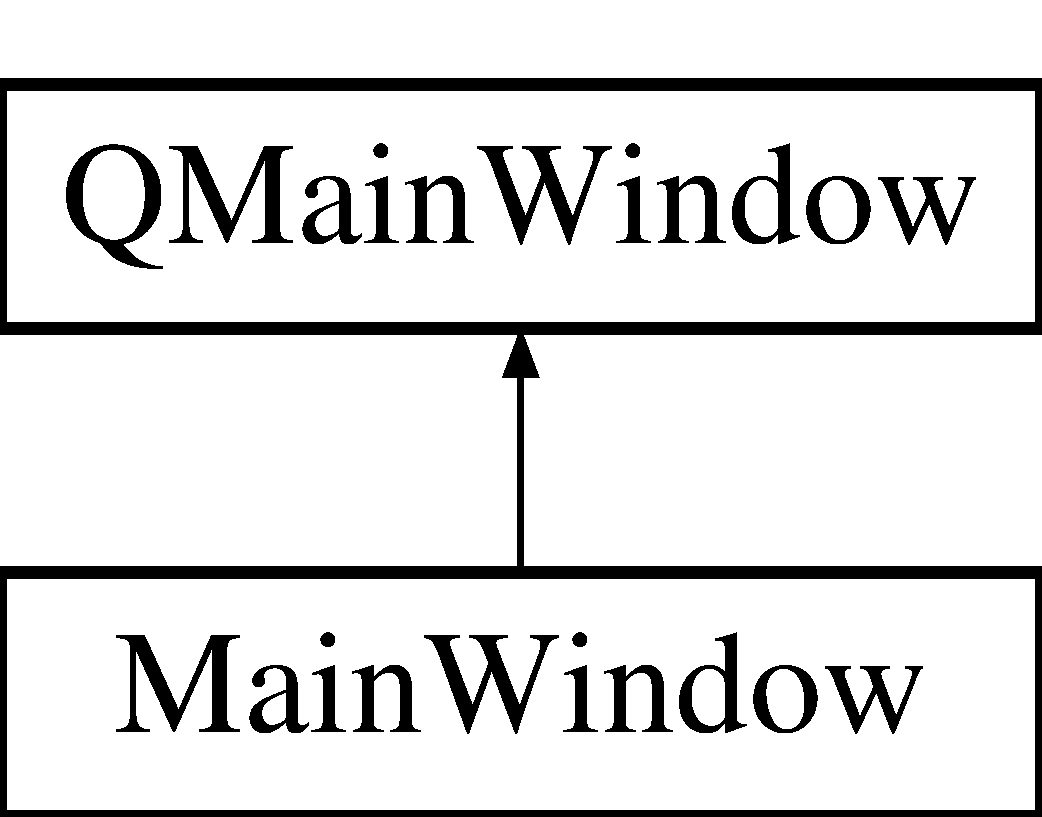
\includegraphics[height=2.000000cm]{d6/d1a/classMainWindow}
\end{center}
\end{figure}
\subsection*{Public Slots}
\begin{DoxyCompactItemize}
\item 
\hypertarget{classMainWindow_a661e495fc5b587dce8c7b930120098aa}{void {\bfseries add\-Customer} ()}\label{classMainWindow_a661e495fc5b587dce8c7b930120098aa}

\item 
\hypertarget{classMainWindow_afff9ca5b1b867af6b54eb1c8d9501522}{void {\bfseries edit\-Customer} ()}\label{classMainWindow_afff9ca5b1b867af6b54eb1c8d9501522}

\item 
\hypertarget{classMainWindow_adb6fcfe64c3a11f28655e397b3accea9}{void {\bfseries remove\-Customer} ()}\label{classMainWindow_adb6fcfe64c3a11f28655e397b3accea9}

\item 
\hypertarget{classMainWindow_ad2f2a4051df4fc4776ea4465cf6b6ecb}{void {\bfseries open\-Customer} ()}\label{classMainWindow_ad2f2a4051df4fc4776ea4465cf6b6ecb}

\item 
\hypertarget{classMainWindow_a32fb574dece506733a3b80d2ccf565ac}{void {\bfseries edit\-User} ()}\label{classMainWindow_a32fb574dece506733a3b80d2ccf565ac}

\item 
\hypertarget{classMainWindow_aa186e57f984c98ea0266536df32acebd}{void {\bfseries search} (Q\-String)}\label{classMainWindow_aa186e57f984c98ea0266536df32acebd}

\item 
\hypertarget{classMainWindow_a274dd0e068ebdc2a752e7ef05209fb2d}{void {\bfseries search} ()}\label{classMainWindow_a274dd0e068ebdc2a752e7ef05209fb2d}

\item 
\hypertarget{classMainWindow_a31a63c4615f9c26a6df6e8c3b52967a1}{void {\bfseries new\-Project} (void)}\label{classMainWindow_a31a63c4615f9c26a6df6e8c3b52967a1}

\item 
\hypertarget{classMainWindow_a4710d90108bd39f7b80bdc6c3a1b1aef}{void {\bfseries about\-Qt} ()}\label{classMainWindow_a4710d90108bd39f7b80bdc6c3a1b1aef}

\item 
\hypertarget{classMainWindow_a82e1b6ba63283af94f37684cf14b5c66}{void {\bfseries about\-Fact} ()}\label{classMainWindow_a82e1b6ba63283af94f37684cf14b5c66}

\item 
\hypertarget{classMainWindow_af9af9644d45d2af769d18f2370eed83e}{void {\bfseries about\-Fact\-Dev} ()}\label{classMainWindow_af9af9644d45d2af769d18f2370eed83e}

\item 
\hypertarget{classMainWindow_ae6a7598b9931ca8901a62bb95c490e0e}{void {\bfseries about\-Icons} ()}\label{classMainWindow_ae6a7598b9931ca8901a62bb95c490e0e}

\item 
\hypertarget{classMainWindow_afa850634f7968a6e9803a25e905f3178}{void {\bfseries change\-Customer} ()}\label{classMainWindow_afa850634f7968a6e9803a25e905f3178}

\end{DoxyCompactItemize}
\subsection*{Public Member Functions}
\begin{DoxyCompactItemize}
\item 
\hypertarget{classMainWindow_a8b244be8b7b7db1b08de2a2acb9409db}{{\bfseries Main\-Window} (Q\-Widget $\ast$parent=0)}\label{classMainWindow_a8b244be8b7b7db1b08de2a2acb9409db}

\item 
\hypertarget{classMainWindow_a0584b17eb78c07b513524a09bd914042}{int {\bfseries get\-Current\-Customer\-Id} ()}\label{classMainWindow_a0584b17eb78c07b513524a09bd914042}

\end{DoxyCompactItemize}


The documentation for this class was generated from the following files\-:\begin{DoxyCompactItemize}
\item 
/home/aroquemaurel/projets/qt/\-Fact\-Dev/src/mainwindow.\-h\item 
/home/aroquemaurel/projets/qt/\-Fact\-Dev/src/mainwindow.\-cpp\end{DoxyCompactItemize}

\hypertarget{classParameters}{\section{Parameters Class Reference}
\label{classParameters}\index{Parameters@{Parameters}}
}
\subsection*{Static Public Attributes}
\begin{DoxyCompactItemize}
\item 
\hypertarget{classParameters_a80b98bd51d910bcc2203afcacbc7df87}{static const Q\-String {\bfseries D\-B\-\_\-\-F\-I\-L\-E\-N\-A\-M\-E} = \char`\"{}database.\-db\char`\"{}}\label{classParameters_a80b98bd51d910bcc2203afcacbc7df87}

\item 
\hypertarget{classParameters_a279ee24140c761de46178daa8960bdc8}{static const double {\bfseries V\-E\-R\-S\-I\-O\-N} = 0.\-1}\label{classParameters_a279ee24140c761de46178daa8960bdc8}

\end{DoxyCompactItemize}


The documentation for this class was generated from the following files\-:\begin{DoxyCompactItemize}
\item 
/home/aroquemaurel/projets/qt/\-Fact\-Dev/src/parameters.\-h\item 
/home/aroquemaurel/projets/qt/\-Fact\-Dev/src/parameters.\-cpp\end{DoxyCompactItemize}

\hypertarget{classPopup}{\section{Popup Class Reference}
\label{classPopup}\index{Popup@{Popup}}
}


Class for display popup quickly.  




{\ttfamily \#include $<$popup.\+h$>$}

\subsection*{Static Public Member Functions}
\begin{DoxyCompactItemize}
\item 
\hypertarget{classPopup_aa3173e0f473b42f08363c4ef17c93a07}{static void \hyperlink{classPopup_aa3173e0f473b42f08363c4ef17c93a07}{to\+Implement} (Q\+String, Q\+Widget $\ast$)}\label{classPopup_aa3173e0f473b42f08363c4ef17c93a07}

\begin{DoxyCompactList}\small\item\em \hyperlink{classPopup_aa3173e0f473b42f08363c4ef17c93a07}{Popup\+::to\+Implement} Method to display a critical message \+: feature is not implemented now. \end{DoxyCompactList}\end{DoxyCompactItemize}


\subsection{Detailed Description}
Class for display popup quickly. 

\begin{DoxyAuthor}{Author}
Antoine de Roquemaurel 
\end{DoxyAuthor}


The documentation for this class was generated from the following files\+:\begin{DoxyCompactItemize}
\item 
src/widgets/popup.\+h\item 
src/widgets/popup.\+cpp\end{DoxyCompactItemize}

\hypertarget{classProject}{\section{Project Class Reference}
\label{classProject}\index{Project@{Project}}
}


The \hyperlink{classProject}{Project} class \+: \hyperlink{classProject}{Project} linked to a \hyperlink{classCustomer}{Customer}.  




{\ttfamily \#include $<$project.\+h$>$}

Inheritance diagram for Project\+:\begin{figure}[H]
\begin{center}
\leavevmode
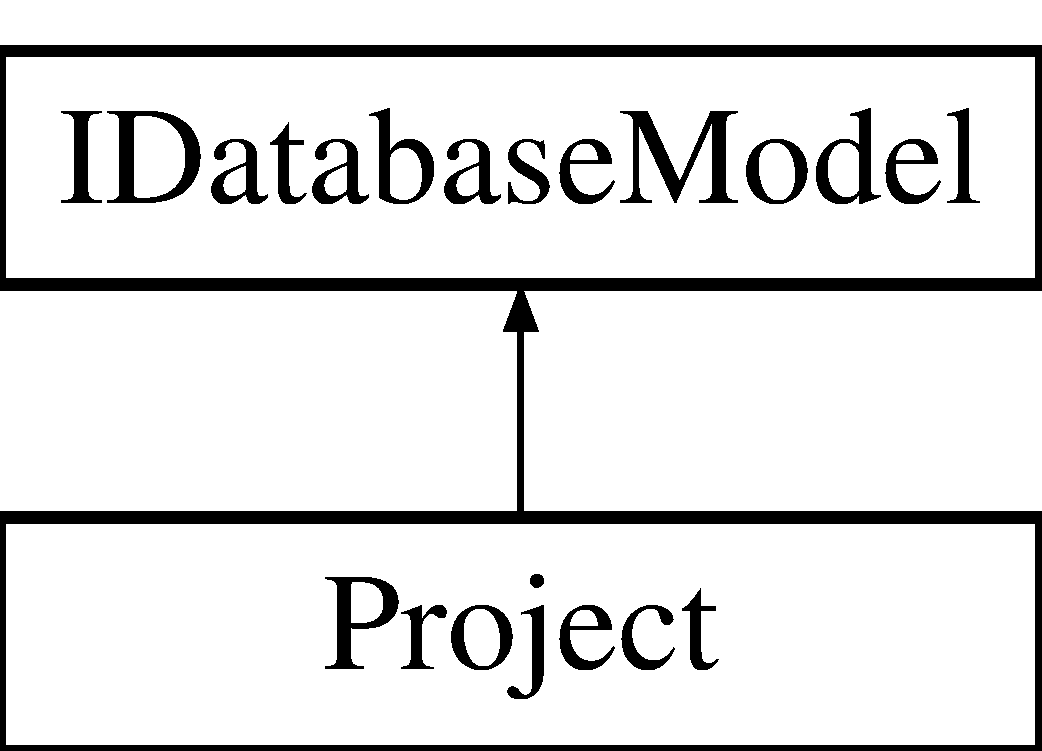
\includegraphics[height=2.000000cm]{db/d91/classProject}
\end{center}
\end{figure}
\subsection*{Public Member Functions}
\begin{DoxyCompactItemize}
\item 
\hypertarget{classProject_aa007ecd17d5bc800e7a956cf666eea21}{\hyperlink{classProject_aa007ecd17d5bc800e7a956cf666eea21}{Project} ()}\label{classProject_aa007ecd17d5bc800e7a956cf666eea21}

\begin{DoxyCompactList}\small\item\em \hyperlink{classProject_aa007ecd17d5bc800e7a956cf666eea21}{Project\+::\+Project} Construct a \hyperlink{classProject}{Project}. \end{DoxyCompactList}\item 
\hyperlink{classProject_a8f608fdf1f0687598294f9534d702dd5}{Project} (int id)
\begin{DoxyCompactList}\small\item\em \hyperlink{classProject_aa007ecd17d5bc800e7a956cf666eea21}{Project\+::\+Project} Construct a \hyperlink{classProject}{Project} which is specified by an {\itshape id} \end{DoxyCompactList}\item 
\hypertarget{classProject_ab471d9354fb128c801f455e9a6bef675}{void \hyperlink{classProject_ab471d9354fb128c801f455e9a6bef675}{commit} ()}\label{classProject_ab471d9354fb128c801f455e9a6bef675}

\begin{DoxyCompactList}\small\item\em \hyperlink{classProject_ab471d9354fb128c801f455e9a6bef675}{Project\+::commit} Update project data in the database. \end{DoxyCompactList}\item 
void \hyperlink{classProject_aa966f15c9c8a277844a75c3530701525}{hydrat} (int id)
\begin{DoxyCompactList}\small\item\em \hyperlink{classProject_aa966f15c9c8a277844a75c3530701525}{Project\+::hydrat} Insert project data which is specified by {\itshape id} in the database. \end{DoxyCompactList}\item 
\hypertarget{classProject_a7bd735a59c2fdf2718db14c3073245fc}{void \hyperlink{classProject_a7bd735a59c2fdf2718db14c3073245fc}{remove} ()}\label{classProject_a7bd735a59c2fdf2718db14c3073245fc}

\begin{DoxyCompactList}\small\item\em \hyperlink{classProject_a7bd735a59c2fdf2718db14c3073245fc}{Project\+::remove} Remove the current project. \end{DoxyCompactList}\item 
Q\+String \hyperlink{classProject_af547be6d3433bbf4ccf0f905788a9fee}{get\+Name} () const 
\begin{DoxyCompactList}\small\item\em \hyperlink{classProject_af547be6d3433bbf4ccf0f905788a9fee}{Project\+::get\+Name} Return the project name. \end{DoxyCompactList}\item 
void \hyperlink{classProject_ab330ed5176b1eb93b558676fff8c47e1}{set\+Name} (const Q\+String \&name)
\begin{DoxyCompactList}\small\item\em \hyperlink{classProject_ab330ed5176b1eb93b558676fff8c47e1}{Project\+::set\+Name} Modify the project {\itshape name} \end{DoxyCompactList}\item 
Q\+String \hyperlink{classProject_ae7cc47cfca8038bf63b67f0d255e92dd}{get\+Description} () const 
\begin{DoxyCompactList}\small\item\em \hyperlink{classProject_ae7cc47cfca8038bf63b67f0d255e92dd}{Project\+::get\+Description} Return a project description. \end{DoxyCompactList}\item 
void \hyperlink{classProject_a08632a8a8905245559c844c863fc796b}{set\+Description} (const Q\+String \&description)
\begin{DoxyCompactList}\small\item\em \hyperlink{classProject_a08632a8a8905245559c844c863fc796b}{Project\+::set\+Description} Modify the project {\itshape description} \end{DoxyCompactList}\item 
double \hyperlink{classProject_a1f34916428682e0134675d45f93a2173}{get\+Daily\+Rate} () const 
\begin{DoxyCompactList}\small\item\em \hyperlink{classProject_a1f34916428682e0134675d45f93a2173}{Project\+::get\+Daily\+Rate} Return the daily rate estimated for this project. \end{DoxyCompactList}\item 
void \hyperlink{classProject_aa3c6dc9722ed16fd69a6034b2398a7c9}{set\+Daily\+Rate} (double daily\+Rate)
\begin{DoxyCompactList}\small\item\em \hyperlink{classProject_aa3c6dc9722ed16fd69a6034b2398a7c9}{Project\+::set\+Daily\+Rate} Modify the daily rate {\itshape daily\+Rate} of the current project. \end{DoxyCompactList}\item 
\hyperlink{classCustomer}{Customer} $\ast$ \hyperlink{classProject_a92b286f48db8f3643214e0c802201d1e}{get\+Customer} () const 
\begin{DoxyCompactList}\small\item\em \hyperlink{classProject_a92b286f48db8f3643214e0c802201d1e}{Project\+::get\+Customer} Return the reference to the customer linked to this project. \end{DoxyCompactList}\item 
void \hyperlink{classProject_a0f1d520c0ecbbfa286d310d18c55dabd}{set\+Customer} (\hyperlink{classCustomer}{Customer} $\ast$customer)
\begin{DoxyCompactList}\small\item\em \hyperlink{classProject_a0f1d520c0ecbbfa286d310d18c55dabd}{Project\+::set\+Customer} Modify the {\itshape customer} linked to this project. \end{DoxyCompactList}\end{DoxyCompactItemize}
\subsection*{Additional Inherited Members}


\subsection{Detailed Description}
The \hyperlink{classProject}{Project} class \+: \hyperlink{classProject}{Project} linked to a \hyperlink{classCustomer}{Customer}. 

\begin{DoxyAuthor}{Author}
Florent Berbie 
\end{DoxyAuthor}
\begin{DoxySeeAlso}{See also}
\hyperlink{classIDatabaseModel}{I\+Database\+Model} 
\end{DoxySeeAlso}


\subsection{Constructor \& Destructor Documentation}
\hypertarget{classProject_a8f608fdf1f0687598294f9534d702dd5}{\index{Project@{Project}!Project@{Project}}
\index{Project@{Project}!Project@{Project}}
\subsubsection[{Project}]{\setlength{\rightskip}{0pt plus 5cm}Project\+::\+Project (
\begin{DoxyParamCaption}
\item[{int}]{id}
\end{DoxyParamCaption}
)}}\label{classProject_a8f608fdf1f0687598294f9534d702dd5}


\hyperlink{classProject_aa007ecd17d5bc800e7a956cf666eea21}{Project\+::\+Project} Construct a \hyperlink{classProject}{Project} which is specified by an {\itshape id} 


\begin{DoxyParams}{Parameters}
{\em id} & \\
\hline
\end{DoxyParams}


\subsection{Member Function Documentation}
\hypertarget{classProject_a92b286f48db8f3643214e0c802201d1e}{\index{Project@{Project}!get\+Customer@{get\+Customer}}
\index{get\+Customer@{get\+Customer}!Project@{Project}}
\subsubsection[{get\+Customer}]{\setlength{\rightskip}{0pt plus 5cm}{\bf Customer} $\ast$ Project\+::get\+Customer (
\begin{DoxyParamCaption}
{}
\end{DoxyParamCaption}
) const}}\label{classProject_a92b286f48db8f3643214e0c802201d1e}


\hyperlink{classProject_a92b286f48db8f3643214e0c802201d1e}{Project\+::get\+Customer} Return the reference to the customer linked to this project. 

\begin{DoxyReturn}{Returns}
customer linked to this project 
\end{DoxyReturn}
\hypertarget{classProject_a1f34916428682e0134675d45f93a2173}{\index{Project@{Project}!get\+Daily\+Rate@{get\+Daily\+Rate}}
\index{get\+Daily\+Rate@{get\+Daily\+Rate}!Project@{Project}}
\subsubsection[{get\+Daily\+Rate}]{\setlength{\rightskip}{0pt plus 5cm}double Project\+::get\+Daily\+Rate (
\begin{DoxyParamCaption}
{}
\end{DoxyParamCaption}
) const}}\label{classProject_a1f34916428682e0134675d45f93a2173}


\hyperlink{classProject_a1f34916428682e0134675d45f93a2173}{Project\+::get\+Daily\+Rate} Return the daily rate estimated for this project. 

\begin{DoxyReturn}{Returns}
the daily rate linket to the current project 
\end{DoxyReturn}
\hypertarget{classProject_ae7cc47cfca8038bf63b67f0d255e92dd}{\index{Project@{Project}!get\+Description@{get\+Description}}
\index{get\+Description@{get\+Description}!Project@{Project}}
\subsubsection[{get\+Description}]{\setlength{\rightskip}{0pt plus 5cm}Q\+String Project\+::get\+Description (
\begin{DoxyParamCaption}
{}
\end{DoxyParamCaption}
) const}}\label{classProject_ae7cc47cfca8038bf63b67f0d255e92dd}


\hyperlink{classProject_ae7cc47cfca8038bf63b67f0d255e92dd}{Project\+::get\+Description} Return a project description. 

\begin{DoxyReturn}{Returns}
project description 
\end{DoxyReturn}
\hypertarget{classProject_af547be6d3433bbf4ccf0f905788a9fee}{\index{Project@{Project}!get\+Name@{get\+Name}}
\index{get\+Name@{get\+Name}!Project@{Project}}
\subsubsection[{get\+Name}]{\setlength{\rightskip}{0pt plus 5cm}Q\+String Project\+::get\+Name (
\begin{DoxyParamCaption}
{}
\end{DoxyParamCaption}
) const}}\label{classProject_af547be6d3433bbf4ccf0f905788a9fee}


\hyperlink{classProject_af547be6d3433bbf4ccf0f905788a9fee}{Project\+::get\+Name} Return the project name. 

\begin{DoxyReturn}{Returns}
project name 
\end{DoxyReturn}
\hypertarget{classProject_aa966f15c9c8a277844a75c3530701525}{\index{Project@{Project}!hydrat@{hydrat}}
\index{hydrat@{hydrat}!Project@{Project}}
\subsubsection[{hydrat}]{\setlength{\rightskip}{0pt plus 5cm}void Project\+::hydrat (
\begin{DoxyParamCaption}
\item[{int}]{id}
\end{DoxyParamCaption}
)\hspace{0.3cm}{\ttfamily [virtual]}}}\label{classProject_aa966f15c9c8a277844a75c3530701525}


\hyperlink{classProject_aa966f15c9c8a277844a75c3530701525}{Project\+::hydrat} Insert project data which is specified by {\itshape id} in the database. 


\begin{DoxyParams}{Parameters}
{\em id} & \hyperlink{classProject}{Project} identify \\
\hline
\end{DoxyParams}


Implements \hyperlink{classIDatabaseModel_a25e44ed10a75976f86e14d34aea02c37}{I\+Database\+Model}.

\hypertarget{classProject_a0f1d520c0ecbbfa286d310d18c55dabd}{\index{Project@{Project}!set\+Customer@{set\+Customer}}
\index{set\+Customer@{set\+Customer}!Project@{Project}}
\subsubsection[{set\+Customer}]{\setlength{\rightskip}{0pt plus 5cm}void Project\+::set\+Customer (
\begin{DoxyParamCaption}
\item[{{\bf Customer} $\ast$}]{customer}
\end{DoxyParamCaption}
)}}\label{classProject_a0f1d520c0ecbbfa286d310d18c55dabd}


\hyperlink{classProject_a0f1d520c0ecbbfa286d310d18c55dabd}{Project\+::set\+Customer} Modify the {\itshape customer} linked to this project. 


\begin{DoxyParams}{Parameters}
{\em customer} & New customer associated to this project \\
\hline
\end{DoxyParams}
\hypertarget{classProject_aa3c6dc9722ed16fd69a6034b2398a7c9}{\index{Project@{Project}!set\+Daily\+Rate@{set\+Daily\+Rate}}
\index{set\+Daily\+Rate@{set\+Daily\+Rate}!Project@{Project}}
\subsubsection[{set\+Daily\+Rate}]{\setlength{\rightskip}{0pt plus 5cm}void Project\+::set\+Daily\+Rate (
\begin{DoxyParamCaption}
\item[{double}]{daily\+Rate}
\end{DoxyParamCaption}
)}}\label{classProject_aa3c6dc9722ed16fd69a6034b2398a7c9}


\hyperlink{classProject_aa3c6dc9722ed16fd69a6034b2398a7c9}{Project\+::set\+Daily\+Rate} Modify the daily rate {\itshape daily\+Rate} of the current project. 


\begin{DoxyParams}{Parameters}
{\em daily\+Rate} & New daily rate associated to the current project \\
\hline
\end{DoxyParams}
\hypertarget{classProject_a08632a8a8905245559c844c863fc796b}{\index{Project@{Project}!set\+Description@{set\+Description}}
\index{set\+Description@{set\+Description}!Project@{Project}}
\subsubsection[{set\+Description}]{\setlength{\rightskip}{0pt plus 5cm}void Project\+::set\+Description (
\begin{DoxyParamCaption}
\item[{const Q\+String \&}]{description}
\end{DoxyParamCaption}
)}}\label{classProject_a08632a8a8905245559c844c863fc796b}


\hyperlink{classProject_a08632a8a8905245559c844c863fc796b}{Project\+::set\+Description} Modify the project {\itshape description} 


\begin{DoxyParams}{Parameters}
{\em description} & New project description \\
\hline
\end{DoxyParams}
\hypertarget{classProject_ab330ed5176b1eb93b558676fff8c47e1}{\index{Project@{Project}!set\+Name@{set\+Name}}
\index{set\+Name@{set\+Name}!Project@{Project}}
\subsubsection[{set\+Name}]{\setlength{\rightskip}{0pt plus 5cm}void Project\+::set\+Name (
\begin{DoxyParamCaption}
\item[{const Q\+String \&}]{name}
\end{DoxyParamCaption}
)}}\label{classProject_ab330ed5176b1eb93b558676fff8c47e1}


\hyperlink{classProject_ab330ed5176b1eb93b558676fff8c47e1}{Project\+::set\+Name} Modify the project {\itshape name} 


\begin{DoxyParams}{Parameters}
{\em name} & \hyperlink{classProject}{Project} name \\
\hline
\end{DoxyParams}


The documentation for this class was generated from the following files\+:\begin{DoxyCompactItemize}
\item 
src/models/project.\+h\item 
src/models/project.\+cpp\end{DoxyCompactItemize}

\hypertarget{classProjectDatabase}{\section{Project\-Database Class Reference}
\label{classProjectDatabase}\index{Project\-Database@{Project\-Database}}
}


The \hyperlink{classProjectDatabase}{Project\-Database} class \hyperlink{classProject}{Project} table database.  




{\ttfamily \#include $<$projectdatabase.\-h$>$}

Inheritance diagram for Project\-Database\-:\begin{figure}[H]
\begin{center}
\leavevmode
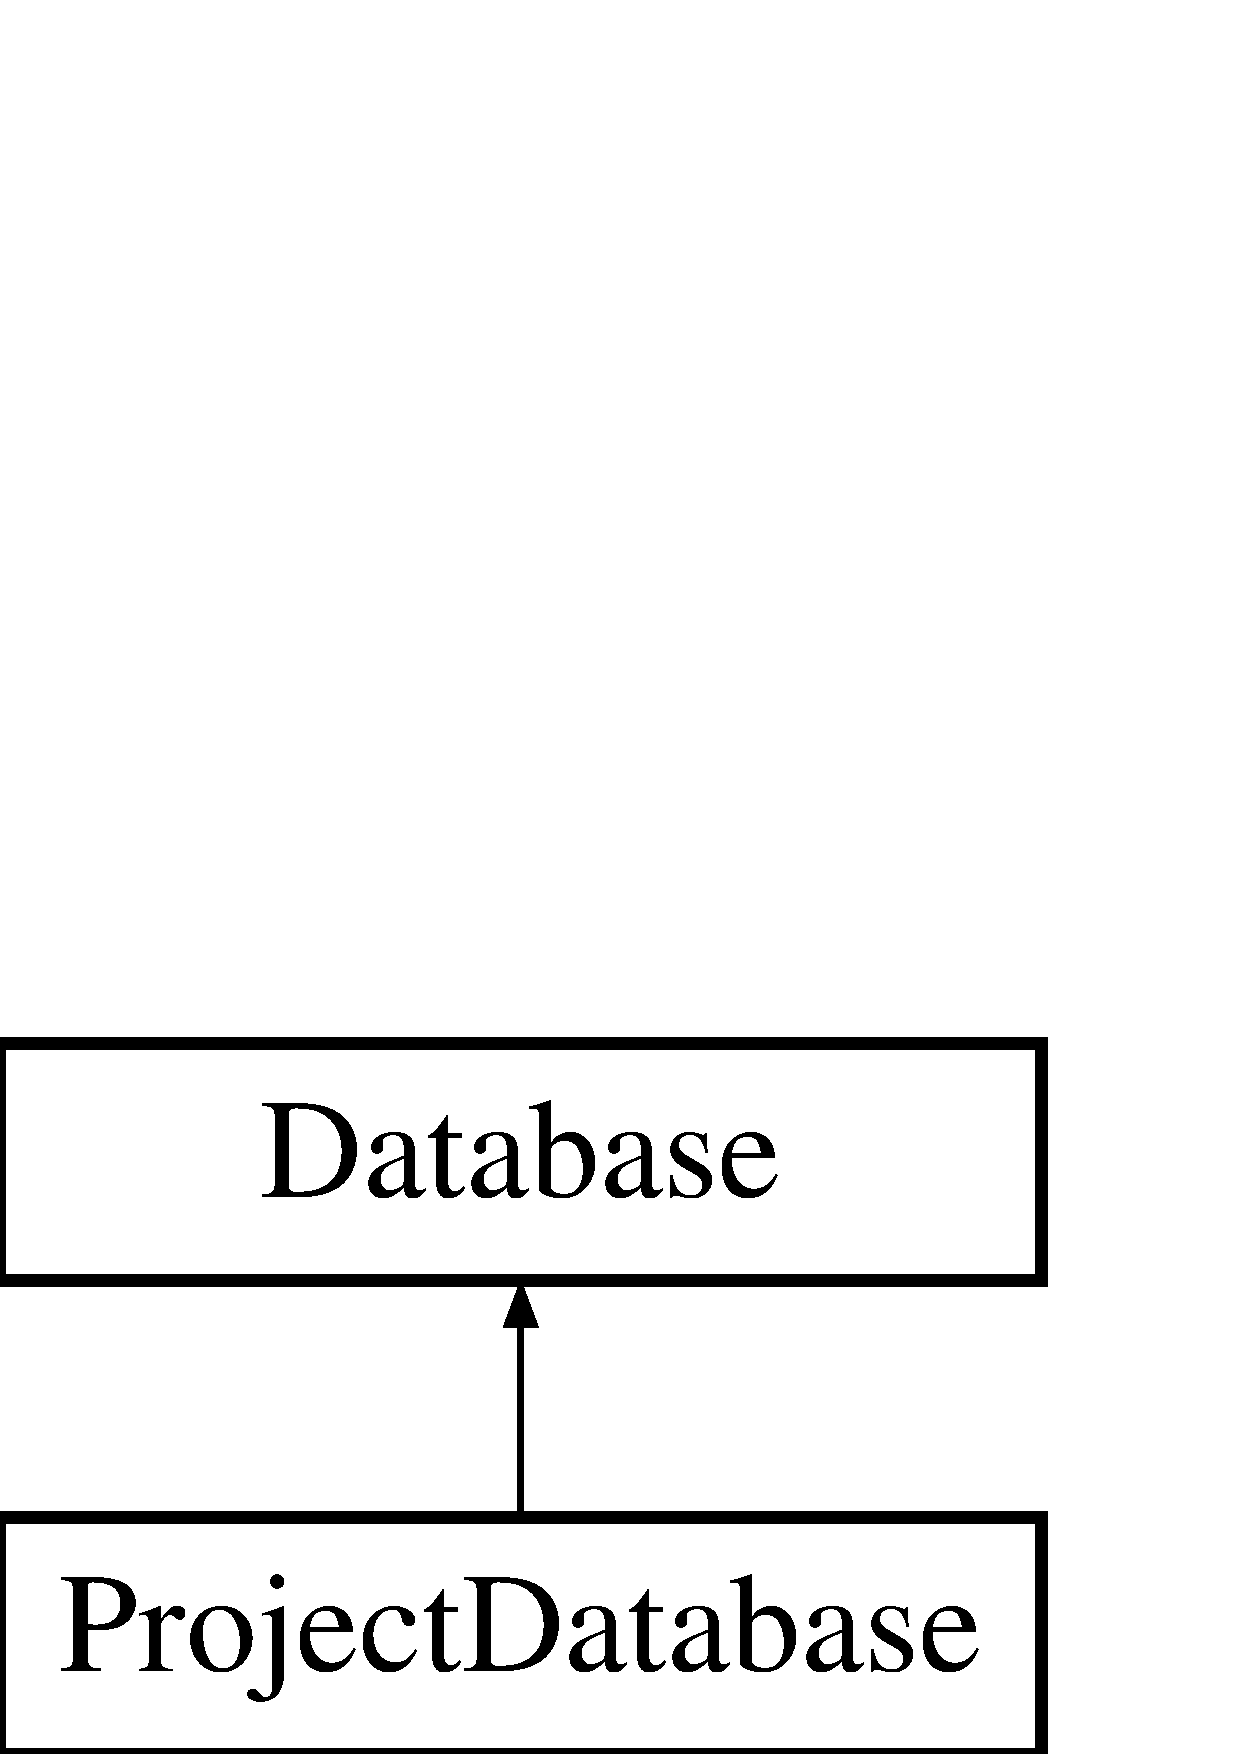
\includegraphics[height=2.000000cm]{d4/d8d/classProjectDatabase}
\end{center}
\end{figure}
\subsection*{Public Member Functions}
\begin{DoxyCompactItemize}
\item 
\hyperlink{classProject}{Project} $\ast$ \hyperlink{classProjectDatabase_a895c03003dc4deea0bc429776337795f}{get\-Project} (const int p\-Id)
\begin{DoxyCompactList}\small\item\em Project\-Databaseget\-Project Get informations about the project identified by 'p\-Id'. \end{DoxyCompactList}\item 
int \hyperlink{classProjectDatabase_a3e2c3d198f7f5724ae0388fd49f4e8cb}{add\-Project} (const \hyperlink{classProject}{Project} \&)
\begin{DoxyCompactList}\small\item\em \hyperlink{classProjectDatabase}{Project\-Database}\-:add\-Project Add the project 'p\-Project' to the database. \end{DoxyCompactList}\item 
\hypertarget{classProjectDatabase_a959b2f9617969277a8c92a8239c613f1}{void \hyperlink{classProjectDatabase_a959b2f9617969277a8c92a8239c613f1}{update\-Project} (const \hyperlink{classProject}{Project} \&)}\label{classProjectDatabase_a959b2f9617969277a8c92a8239c613f1}

\begin{DoxyCompactList}\small\item\em \hyperlink{classProjectDatabase}{Project\-Database}\-:update\-Project Update informations about the project. \end{DoxyCompactList}\item 
void \hyperlink{classProjectDatabase_a52f3c3b312c418568531eb4cd2ecf615}{remove\-Project} (const int p\-Id)
\begin{DoxyCompactList}\small\item\em remove\-Project Remove the project with the id 'p\-Id' \end{DoxyCompactList}\item 
int \hyperlink{classProjectDatabase_a48ab28fa18bc3f0371f8c17c5421a46e}{get\-Nb\-Projects} ()
\begin{DoxyCompactList}\small\item\em \hyperlink{classProjectDatabase}{Project\-Database}\-:get\-Nb\-Projects Return the number of projects existing. \end{DoxyCompactList}\item 
int \hyperlink{classProjectDatabase_a3dbf2e270674727fc479d392c6609dec}{get\-Nb\-Projects\-For\-A\-Customer} (const int p\-Id)
\begin{DoxyCompactList}\small\item\em \hyperlink{classProjectDatabase}{Project\-Database}\-:get\-Nb\-Projects\-For\-A\-Customer Return the number of projects existing for an identify customer {\itshape p\-Id} \end{DoxyCompactList}\end{DoxyCompactItemize}
\subsection*{Static Public Member Functions}
\begin{DoxyCompactItemize}
\item 
static \hyperlink{classProjectDatabase}{Project\-Database} $\ast$ \hyperlink{classProjectDatabase_a06a93b599475687f19f66c7bbb921899}{instance} ()  throw (\-Db\-Exception$\ast$)
\begin{DoxyCompactList}\small\item\em Project\-Database\-::get\-Instance Return an instance of \hyperlink{classProjectDatabase}{Project\-Database}. \end{DoxyCompactList}\end{DoxyCompactItemize}
\subsection*{Additional Inherited Members}


\subsection{Detailed Description}
The \hyperlink{classProjectDatabase}{Project\-Database} class \hyperlink{classProject}{Project} table database. 

\begin{DoxyAuthor}{Author}
Florent Berbie 
\end{DoxyAuthor}
\begin{DoxySeeAlso}{See Also}
\hyperlink{classDatabase}{Database} 

\hyperlink{classProject}{Project} 
\end{DoxySeeAlso}


\subsection{Member Function Documentation}
\hypertarget{classProjectDatabase_a3e2c3d198f7f5724ae0388fd49f4e8cb}{\index{Project\-Database@{Project\-Database}!add\-Project@{add\-Project}}
\index{add\-Project@{add\-Project}!ProjectDatabase@{Project\-Database}}
\subsubsection[{add\-Project}]{\setlength{\rightskip}{0pt plus 5cm}int Project\-Database\-::add\-Project (
\begin{DoxyParamCaption}
\item[{const {\bf Project} \&}]{p\-Project}
\end{DoxyParamCaption}
)}}\label{classProjectDatabase_a3e2c3d198f7f5724ae0388fd49f4e8cb}


\hyperlink{classProjectDatabase}{Project\-Database}\-:add\-Project Add the project 'p\-Project' to the database. 

\begin{DoxyReturn}{Returns}
project id 
\end{DoxyReturn}
\hypertarget{classProjectDatabase_a48ab28fa18bc3f0371f8c17c5421a46e}{\index{Project\-Database@{Project\-Database}!get\-Nb\-Projects@{get\-Nb\-Projects}}
\index{get\-Nb\-Projects@{get\-Nb\-Projects}!ProjectDatabase@{Project\-Database}}
\subsubsection[{get\-Nb\-Projects}]{\setlength{\rightskip}{0pt plus 5cm}int Project\-Database\-::get\-Nb\-Projects (
\begin{DoxyParamCaption}
{}
\end{DoxyParamCaption}
)}}\label{classProjectDatabase_a48ab28fa18bc3f0371f8c17c5421a46e}


\hyperlink{classProjectDatabase}{Project\-Database}\-:get\-Nb\-Projects Return the number of projects existing. 

\begin{DoxyReturn}{Returns}
number of projects 
\end{DoxyReturn}
\hypertarget{classProjectDatabase_a3dbf2e270674727fc479d392c6609dec}{\index{Project\-Database@{Project\-Database}!get\-Nb\-Projects\-For\-A\-Customer@{get\-Nb\-Projects\-For\-A\-Customer}}
\index{get\-Nb\-Projects\-For\-A\-Customer@{get\-Nb\-Projects\-For\-A\-Customer}!ProjectDatabase@{Project\-Database}}
\subsubsection[{get\-Nb\-Projects\-For\-A\-Customer}]{\setlength{\rightskip}{0pt plus 5cm}int Project\-Database\-::get\-Nb\-Projects\-For\-A\-Customer (
\begin{DoxyParamCaption}
\item[{const int}]{p\-Id}
\end{DoxyParamCaption}
)}}\label{classProjectDatabase_a3dbf2e270674727fc479d392c6609dec}


\hyperlink{classProjectDatabase}{Project\-Database}\-:get\-Nb\-Projects\-For\-A\-Customer Return the number of projects existing for an identify customer {\itshape p\-Id} 


\begin{DoxyParams}{Parameters}
{\em p\-Id} & \hyperlink{classProject}{Project} id \\
\hline
\end{DoxyParams}
\begin{DoxyReturn}{Returns}
number of projects 
\end{DoxyReturn}
\hypertarget{classProjectDatabase_a895c03003dc4deea0bc429776337795f}{\index{Project\-Database@{Project\-Database}!get\-Project@{get\-Project}}
\index{get\-Project@{get\-Project}!ProjectDatabase@{Project\-Database}}
\subsubsection[{get\-Project}]{\setlength{\rightskip}{0pt plus 5cm}{\bf Project} $\ast$ Project\-Database\-::get\-Project (
\begin{DoxyParamCaption}
\item[{const int}]{p\-Id}
\end{DoxyParamCaption}
)}}\label{classProjectDatabase_a895c03003dc4deea0bc429776337795f}


Project\-Databaseget\-Project Get informations about the project identified by 'p\-Id'. 


\begin{DoxyParams}{Parameters}
{\em p\-Id} & project \\
\hline
\end{DoxyParams}
\begin{DoxyReturn}{Returns}
the project 
\end{DoxyReturn}
\hypertarget{classProjectDatabase_a06a93b599475687f19f66c7bbb921899}{\index{Project\-Database@{Project\-Database}!instance@{instance}}
\index{instance@{instance}!ProjectDatabase@{Project\-Database}}
\subsubsection[{instance}]{\setlength{\rightskip}{0pt plus 5cm}{\bf Project\-Database} $\ast$ Project\-Database\-::instance (
\begin{DoxyParamCaption}
{}
\end{DoxyParamCaption}
) throw  {\bf Db\-Exception} $\ast$) \hspace{0.3cm}{\ttfamily [static]}}}\label{classProjectDatabase_a06a93b599475687f19f66c7bbb921899}


Project\-Database\-::get\-Instance Return an instance of \hyperlink{classProjectDatabase}{Project\-Database}. 

\begin{DoxyReturn}{Returns}
Instance of \hyperlink{classProjectDatabase}{Project\-Database} 
\end{DoxyReturn}
\hypertarget{classProjectDatabase_a52f3c3b312c418568531eb4cd2ecf615}{\index{Project\-Database@{Project\-Database}!remove\-Project@{remove\-Project}}
\index{remove\-Project@{remove\-Project}!ProjectDatabase@{Project\-Database}}
\subsubsection[{remove\-Project}]{\setlength{\rightskip}{0pt plus 5cm}void Project\-Database\-::remove\-Project (
\begin{DoxyParamCaption}
\item[{const int}]{p\-Id}
\end{DoxyParamCaption}
)}}\label{classProjectDatabase_a52f3c3b312c418568531eb4cd2ecf615}


remove\-Project Remove the project with the id 'p\-Id' 


\begin{DoxyParams}{Parameters}
{\em p\-Id} & project id \\
\hline
\end{DoxyParams}


The documentation for this class was generated from the following files\-:\begin{DoxyCompactItemize}
\item 
/home/florent/\-Documents/\-Projet\-\_\-\-S8/\-Fact\-Dev/src/database/projectdatabase.\-h\item 
/home/florent/\-Documents/\-Projet\-\_\-\-S8/\-Fact\-Dev/src/database/projectdatabase.\-cpp\end{DoxyCompactItemize}

\hypertarget{classProjectsWidget}{\section{Projects\+Widget Class Reference}
\label{classProjectsWidget}\index{Projects\+Widget@{Projects\+Widget}}
}
Inheritance diagram for Projects\+Widget\+:\begin{figure}[H]
\begin{center}
\leavevmode
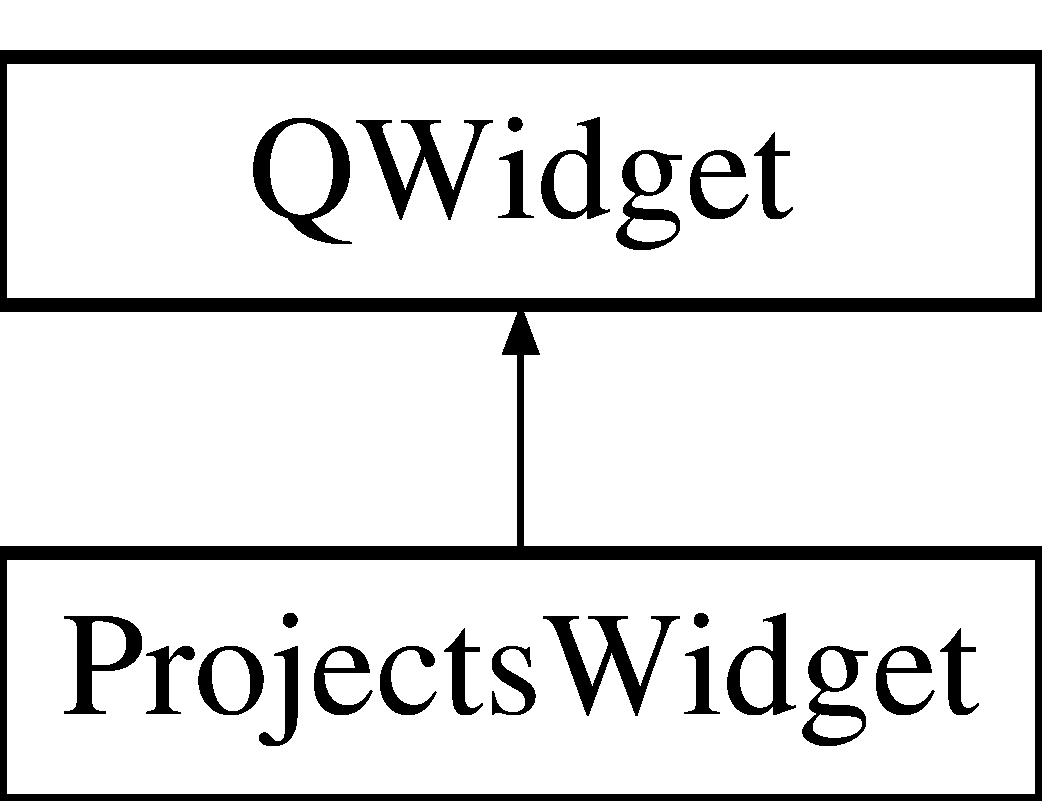
\includegraphics[height=2.000000cm]{de/da7/classProjectsWidget}
\end{center}
\end{figure}
\subsection*{Public Slots}
\begin{DoxyCompactItemize}
\item 
\hypertarget{classProjectsWidget_a9a3e158093ed435a68d4d9874a22a128}{void {\bfseries new\+Project} ()}\label{classProjectsWidget_a9a3e158093ed435a68d4d9874a22a128}

\item 
\hypertarget{classProjectsWidget_a026e17f035717e382f4afca6896a72d3}{void {\bfseries edit\+Selected\+Project} ()}\label{classProjectsWidget_a026e17f035717e382f4afca6896a72d3}

\item 
\hypertarget{classProjectsWidget_a038205ca1dee68dadae84e31dabfd7fc}{void {\bfseries remove\+Selected\+Project} ()}\label{classProjectsWidget_a038205ca1dee68dadae84e31dabfd7fc}

\end{DoxyCompactItemize}
\subsection*{Public Member Functions}
\begin{DoxyCompactItemize}
\item 
\hypertarget{classProjectsWidget_a542fb678c61897b56c86dc58524bd969}{{\bfseries Projects\+Widget} (Q\+Widget $\ast$parent=0)}\label{classProjectsWidget_a542fb678c61897b56c86dc58524bd969}

\end{DoxyCompactItemize}


The documentation for this class was generated from the following files\+:\begin{DoxyCompactItemize}
\item 
src/widgets/projectswidget.\+h\item 
src/widgets/projectswidget.\+cpp\end{DoxyCompactItemize}

\hypertarget{classRateWidget}{\section{Rate\+Widget Class Reference}
\label{classRateWidget}\index{Rate\+Widget@{Rate\+Widget}}
}


Class for display Rate.  




{\ttfamily \#include $<$ratewidget.\+h$>$}

Inheritance diagram for Rate\+Widget\+:\begin{figure}[H]
\begin{center}
\leavevmode
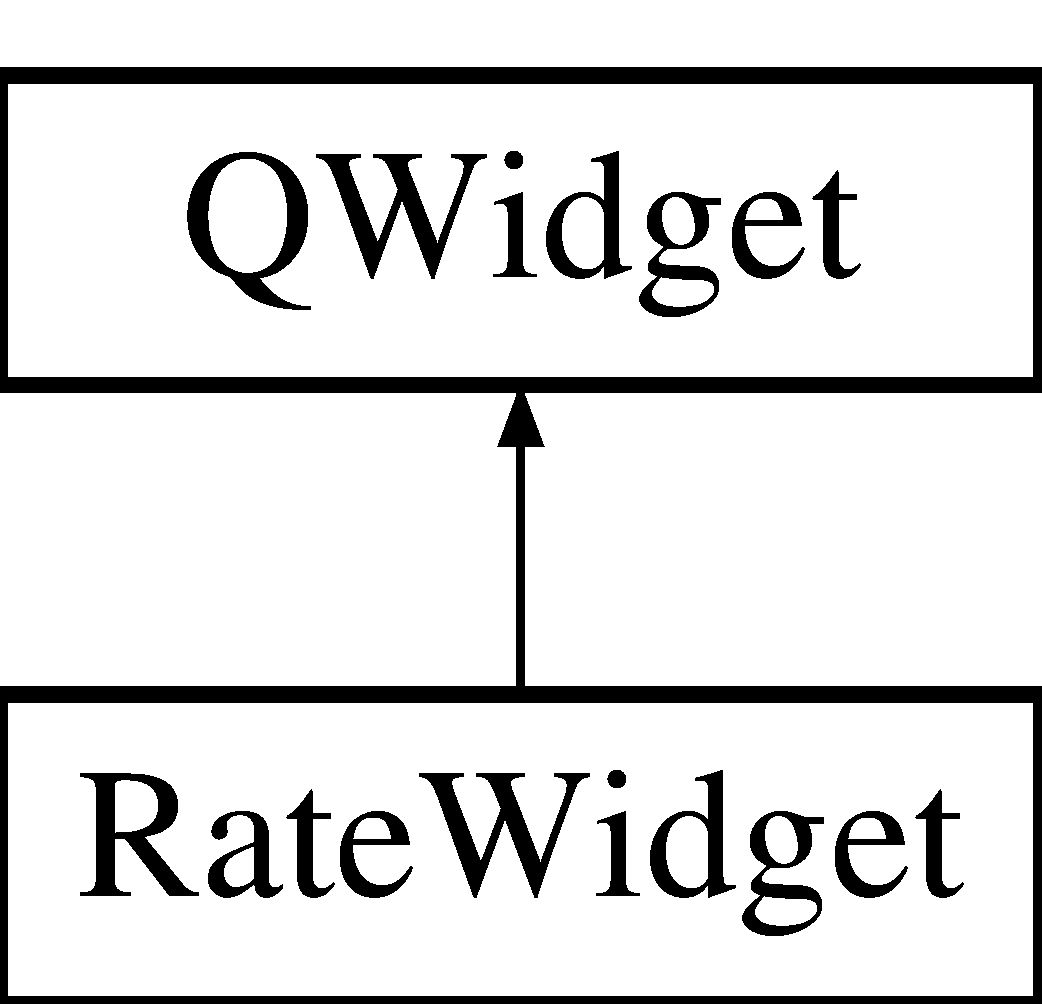
\includegraphics[height=2.000000cm]{dc/da5/classRateWidget}
\end{center}
\end{figure}
\subsection*{Public Member Functions}
\begin{DoxyCompactItemize}
\item 
\hyperlink{classRateWidget_ad1cb6a97e47b408043e83708ff8af15e}{Rate\+Widget} (Q\+Widget $\ast$parent=0)
\begin{DoxyCompactList}\small\item\em \hyperlink{classRateWidget}{Rate\+Widget} Construct a rate widget. \end{DoxyCompactList}\item 
\hypertarget{classRateWidget_a4a3ec9a546055d6ecb3bd1a9ee8082a6}{void \hyperlink{classRateWidget_a4a3ec9a546055d6ecb3bd1a9ee8082a6}{init\+Rate} ()}\label{classRateWidget_a4a3ec9a546055d6ecb3bd1a9ee8082a6}

\begin{DoxyCompactList}\small\item\em init\+Rate Initialize the rate \end{DoxyCompactList}\item 
double \hyperlink{classRateWidget_a0a72cea5ff524b47e513dcb21aea2022}{get\+Daily\+Rate} ()
\begin{DoxyCompactList}\small\item\em get\+Daily\+Rate \end{DoxyCompactList}\item 
void \hyperlink{classRateWidget_a8a3bccabb5c33e9f617ed85a68398b5a}{set\+Daily\+Rate} (double daily\+Rate)
\begin{DoxyCompactList}\small\item\em set\+Daily\+Rate Set a new value for the daily rate \end{DoxyCompactList}\item 
double \hyperlink{classRateWidget_a50285d4472979e004c706ff5640e8227}{get\+Hourly\+Rate} ()
\begin{DoxyCompactList}\small\item\em get\+Hourly\+Rate \end{DoxyCompactList}\item 
void \hyperlink{classRateWidget_a8135738c8a54389110de6751d9e2728e}{set\+Hourly\+Rate} (double hourly\+Rate)
\begin{DoxyCompactList}\small\item\em set\+Hourly\+Rate Set a new value for the hourly rate \end{DoxyCompactList}\end{DoxyCompactItemize}


\subsection{Detailed Description}
Class for display Rate. 

\begin{DoxyAuthor}{Author}
Florent Berbie 
\end{DoxyAuthor}


\subsection{Constructor \& Destructor Documentation}
\hypertarget{classRateWidget_ad1cb6a97e47b408043e83708ff8af15e}{\index{Rate\+Widget@{Rate\+Widget}!Rate\+Widget@{Rate\+Widget}}
\index{Rate\+Widget@{Rate\+Widget}!Rate\+Widget@{Rate\+Widget}}
\subsubsection[{Rate\+Widget}]{\setlength{\rightskip}{0pt plus 5cm}Rate\+Widget\+::\+Rate\+Widget (
\begin{DoxyParamCaption}
\item[{Q\+Widget $\ast$}]{parent = {\ttfamily 0}}
\end{DoxyParamCaption}
)\hspace{0.3cm}{\ttfamily [explicit]}}}\label{classRateWidget_ad1cb6a97e47b408043e83708ff8af15e}


\hyperlink{classRateWidget}{Rate\+Widget} Construct a rate widget. 


\begin{DoxyParams}{Parameters}
{\em parent} & The Q\+Widget parent \\
\hline
\end{DoxyParams}


\subsection{Member Function Documentation}
\hypertarget{classRateWidget_a0a72cea5ff524b47e513dcb21aea2022}{\index{Rate\+Widget@{Rate\+Widget}!get\+Daily\+Rate@{get\+Daily\+Rate}}
\index{get\+Daily\+Rate@{get\+Daily\+Rate}!Rate\+Widget@{Rate\+Widget}}
\subsubsection[{get\+Daily\+Rate}]{\setlength{\rightskip}{0pt plus 5cm}double Rate\+Widget\+::get\+Daily\+Rate (
\begin{DoxyParamCaption}
{}
\end{DoxyParamCaption}
)}}\label{classRateWidget_a0a72cea5ff524b47e513dcb21aea2022}


get\+Daily\+Rate 

\begin{DoxyReturn}{Returns}
The daily rate 
\end{DoxyReturn}
\hypertarget{classRateWidget_a50285d4472979e004c706ff5640e8227}{\index{Rate\+Widget@{Rate\+Widget}!get\+Hourly\+Rate@{get\+Hourly\+Rate}}
\index{get\+Hourly\+Rate@{get\+Hourly\+Rate}!Rate\+Widget@{Rate\+Widget}}
\subsubsection[{get\+Hourly\+Rate}]{\setlength{\rightskip}{0pt plus 5cm}double Rate\+Widget\+::get\+Hourly\+Rate (
\begin{DoxyParamCaption}
{}
\end{DoxyParamCaption}
)}}\label{classRateWidget_a50285d4472979e004c706ff5640e8227}


get\+Hourly\+Rate 

\begin{DoxyReturn}{Returns}
The hourly rate 
\end{DoxyReturn}
\hypertarget{classRateWidget_a8a3bccabb5c33e9f617ed85a68398b5a}{\index{Rate\+Widget@{Rate\+Widget}!set\+Daily\+Rate@{set\+Daily\+Rate}}
\index{set\+Daily\+Rate@{set\+Daily\+Rate}!Rate\+Widget@{Rate\+Widget}}
\subsubsection[{set\+Daily\+Rate}]{\setlength{\rightskip}{0pt plus 5cm}void Rate\+Widget\+::set\+Daily\+Rate (
\begin{DoxyParamCaption}
\item[{double}]{daily\+Rate}
\end{DoxyParamCaption}
)}}\label{classRateWidget_a8a3bccabb5c33e9f617ed85a68398b5a}


set\+Daily\+Rate Set a new value for the daily rate 


\begin{DoxyParams}{Parameters}
{\em daily\+Rate} & The new daily rate \\
\hline
\end{DoxyParams}
\hypertarget{classRateWidget_a8135738c8a54389110de6751d9e2728e}{\index{Rate\+Widget@{Rate\+Widget}!set\+Hourly\+Rate@{set\+Hourly\+Rate}}
\index{set\+Hourly\+Rate@{set\+Hourly\+Rate}!Rate\+Widget@{Rate\+Widget}}
\subsubsection[{set\+Hourly\+Rate}]{\setlength{\rightskip}{0pt plus 5cm}void Rate\+Widget\+::set\+Hourly\+Rate (
\begin{DoxyParamCaption}
\item[{double}]{hourly\+Rate}
\end{DoxyParamCaption}
)}}\label{classRateWidget_a8135738c8a54389110de6751d9e2728e}


set\+Hourly\+Rate Set a new value for the hourly rate 


\begin{DoxyParams}{Parameters}
{\em hourly\+Rate} & The new hourly rate \\
\hline
\end{DoxyParams}


The documentation for this class was generated from the following files\+:\begin{DoxyCompactItemize}
\item 
src/widgets/ratewidget.\+h\item 
src/widgets/ratewidget.\+cpp\end{DoxyCompactItemize}

\hypertarget{classSearch}{\section{Search Class Reference}
\label{classSearch}\index{Search@{Search}}
}


The \hyperlink{classSearch}{Search} class.  




{\ttfamily \#include $<$search.\+h$>$}

\subsection*{Public Member Functions}
\begin{DoxyCompactItemize}
\item 
\hypertarget{classSearch_af629e7254d367d2b2cacfb0699c9de31}{\hyperlink{classSearch_af629e7254d367d2b2cacfb0699c9de31}{Search} ()}\label{classSearch_af629e7254d367d2b2cacfb0699c9de31}

\begin{DoxyCompactList}\small\item\em \hyperlink{classSearch_af629e7254d367d2b2cacfb0699c9de31}{Search\+::\+Search} Construct a search. \end{DoxyCompactList}\item 
\hypertarget{classSearch_afd7e16f7369d7a44189e530292b5faa0}{\hyperlink{classSearch_afd7e16f7369d7a44189e530292b5faa0}{$\sim$\+Search} ()}\label{classSearch_afd7e16f7369d7a44189e530292b5faa0}

\begin{DoxyCompactList}\small\item\em \hyperlink{classSearch_af629e7254d367d2b2cacfb0699c9de31}{Search\+::\+Search} Destruct a search. \end{DoxyCompactList}\item 
Q\+String \hyperlink{classSearch_ad4cbed03998957eb80a2d1b536407f01}{get\+Filter} ()
\begin{DoxyCompactList}\small\item\em \hyperlink{classSearch_ad4cbed03998957eb80a2d1b536407f01}{Search\+::get\+Filter} Return the search filter. \end{DoxyCompactList}\item 
bool \hyperlink{classSearch_a683100feb68358d1eedda781f700cd46}{get\+Search\+In\+Companies} () const 
\begin{DoxyCompactList}\small\item\em \hyperlink{classSearch_a683100feb68358d1eedda781f700cd46}{Search\+::get\+Search\+In\+Companies} Return if we search a company. \end{DoxyCompactList}\item 
void \hyperlink{classSearch_a1c2abc83b8995d5b1d908905a7212042}{set\+Search\+In\+Companies} (bool \hyperlink{classSearch_a683100feb68358d1eedda781f700cd46}{get\+Search\+In\+Companies})
\begin{DoxyCompactList}\small\item\em \hyperlink{classSearch_a1c2abc83b8995d5b1d908905a7212042}{Search\+::set\+Search\+In\+Companies} Modify the filter of search. \end{DoxyCompactList}\item 
bool \hyperlink{classSearch_afb76798798f03d34f8d2363d7062ec0f}{get\+Search\+In\+Referent\+Lastname} () const 
\begin{DoxyCompactList}\small\item\em \hyperlink{classSearch_afb76798798f03d34f8d2363d7062ec0f}{Search\+::get\+Search\+In\+Referent\+Lastname} Return if we search a Last name referent. \end{DoxyCompactList}\item 
void \hyperlink{classSearch_a18603321d8e2039b181dbfe082689a08}{set\+Search\+In\+Referent\+Lastname} (bool \hyperlink{classSearch_afb76798798f03d34f8d2363d7062ec0f}{get\+Search\+In\+Referent\+Lastname})
\begin{DoxyCompactList}\small\item\em \hyperlink{classSearch_a18603321d8e2039b181dbfe082689a08}{Search\+::set\+Search\+In\+Referent\+Lastname} Modify the filter of search. \end{DoxyCompactList}\item 
bool \hyperlink{classSearch_a19db0f8c76c414514b9df09e07b4d962}{get\+Group\+Filter} () const 
\begin{DoxyCompactList}\small\item\em \hyperlink{classSearch_a19db0f8c76c414514b9df09e07b4d962}{Search\+::get\+Group\+Filter} Return if the filter is actived. \end{DoxyCompactList}\item 
void \hyperlink{classSearch_a8a944b2ece0cafe967afb4334d92b62a}{set\+Group\+Filter} (bool \hyperlink{classSearch_a19db0f8c76c414514b9df09e07b4d962}{get\+Group\+Filter})
\begin{DoxyCompactList}\small\item\em \hyperlink{classSearch_a8a944b2ece0cafe967afb4334d92b62a}{Search\+::set\+Group\+Filter} Modify if we active search filter. \end{DoxyCompactList}\item 
Q\+String \hyperlink{classSearch_a10a8f699332477cab0d512027bdaaa44}{get\+Text} () const 
\begin{DoxyCompactList}\small\item\em \hyperlink{classSearch_a10a8f699332477cab0d512027bdaaa44}{Search\+::get\+Text} Return sql portion of filter. \end{DoxyCompactList}\item 
void \hyperlink{classSearch_a92f09448baccf5cddbc433835b716b36}{set\+Text} (const Q\+String \&\hyperlink{classSearch_a10a8f699332477cab0d512027bdaaa44}{get\+Text})
\begin{DoxyCompactList}\small\item\em \hyperlink{classSearch_a92f09448baccf5cddbc433835b716b36}{Search\+::set\+Text} Modify sql portion. \end{DoxyCompactList}\end{DoxyCompactItemize}


\subsection{Detailed Description}
The \hyperlink{classSearch}{Search} class. 

\begin{DoxyAuthor}{Author}
Antoine de Roquemaurel 
\end{DoxyAuthor}


\subsection{Member Function Documentation}
\hypertarget{classSearch_ad4cbed03998957eb80a2d1b536407f01}{\index{Search@{Search}!get\+Filter@{get\+Filter}}
\index{get\+Filter@{get\+Filter}!Search@{Search}}
\subsubsection[{get\+Filter}]{\setlength{\rightskip}{0pt plus 5cm}Q\+String Search\+::get\+Filter (
\begin{DoxyParamCaption}
{}
\end{DoxyParamCaption}
)}}\label{classSearch_ad4cbed03998957eb80a2d1b536407f01}


\hyperlink{classSearch_ad4cbed03998957eb80a2d1b536407f01}{Search\+::get\+Filter} Return the search filter. 

\begin{DoxyReturn}{Returns}
filter selected (sql portion) 
\end{DoxyReturn}
\hypertarget{classSearch_a19db0f8c76c414514b9df09e07b4d962}{\index{Search@{Search}!get\+Group\+Filter@{get\+Group\+Filter}}
\index{get\+Group\+Filter@{get\+Group\+Filter}!Search@{Search}}
\subsubsection[{get\+Group\+Filter}]{\setlength{\rightskip}{0pt plus 5cm}bool Search\+::get\+Group\+Filter (
\begin{DoxyParamCaption}
{}
\end{DoxyParamCaption}
) const}}\label{classSearch_a19db0f8c76c414514b9df09e07b4d962}


\hyperlink{classSearch_a19db0f8c76c414514b9df09e07b4d962}{Search\+::get\+Group\+Filter} Return if the filter is actived. 

\begin{DoxyReturn}{Returns}
boolean if search filter is actived 
\end{DoxyReturn}
\hypertarget{classSearch_a683100feb68358d1eedda781f700cd46}{\index{Search@{Search}!get\+Search\+In\+Companies@{get\+Search\+In\+Companies}}
\index{get\+Search\+In\+Companies@{get\+Search\+In\+Companies}!Search@{Search}}
\subsubsection[{get\+Search\+In\+Companies}]{\setlength{\rightskip}{0pt plus 5cm}bool Search\+::get\+Search\+In\+Companies (
\begin{DoxyParamCaption}
{}
\end{DoxyParamCaption}
) const}}\label{classSearch_a683100feb68358d1eedda781f700cd46}


\hyperlink{classSearch_a683100feb68358d1eedda781f700cd46}{Search\+::get\+Search\+In\+Companies} Return if we search a company. 

\begin{DoxyReturn}{Returns}
boolean if we search a company 
\end{DoxyReturn}
\hypertarget{classSearch_afb76798798f03d34f8d2363d7062ec0f}{\index{Search@{Search}!get\+Search\+In\+Referent\+Lastname@{get\+Search\+In\+Referent\+Lastname}}
\index{get\+Search\+In\+Referent\+Lastname@{get\+Search\+In\+Referent\+Lastname}!Search@{Search}}
\subsubsection[{get\+Search\+In\+Referent\+Lastname}]{\setlength{\rightskip}{0pt plus 5cm}bool Search\+::get\+Search\+In\+Referent\+Lastname (
\begin{DoxyParamCaption}
{}
\end{DoxyParamCaption}
) const}}\label{classSearch_afb76798798f03d34f8d2363d7062ec0f}


\hyperlink{classSearch_afb76798798f03d34f8d2363d7062ec0f}{Search\+::get\+Search\+In\+Referent\+Lastname} Return if we search a Last name referent. 

\begin{DoxyReturn}{Returns}
boolean if search concerns the last name of referent 
\end{DoxyReturn}
\hypertarget{classSearch_a10a8f699332477cab0d512027bdaaa44}{\index{Search@{Search}!get\+Text@{get\+Text}}
\index{get\+Text@{get\+Text}!Search@{Search}}
\subsubsection[{get\+Text}]{\setlength{\rightskip}{0pt plus 5cm}Q\+String Search\+::get\+Text (
\begin{DoxyParamCaption}
{}
\end{DoxyParamCaption}
) const}}\label{classSearch_a10a8f699332477cab0d512027bdaaa44}


\hyperlink{classSearch_a10a8f699332477cab0d512027bdaaa44}{Search\+::get\+Text} Return sql portion of filter. 

\begin{DoxyReturn}{Returns}
Q\+String the sql portion 
\end{DoxyReturn}
\hypertarget{classSearch_a8a944b2ece0cafe967afb4334d92b62a}{\index{Search@{Search}!set\+Group\+Filter@{set\+Group\+Filter}}
\index{set\+Group\+Filter@{set\+Group\+Filter}!Search@{Search}}
\subsubsection[{set\+Group\+Filter}]{\setlength{\rightskip}{0pt plus 5cm}void Search\+::set\+Group\+Filter (
\begin{DoxyParamCaption}
\item[{bool}]{get\+Group\+Filter}
\end{DoxyParamCaption}
)}}\label{classSearch_a8a944b2ece0cafe967afb4334d92b62a}


\hyperlink{classSearch_a8a944b2ece0cafe967afb4334d92b62a}{Search\+::set\+Group\+Filter} Modify if we active search filter. 


\begin{DoxyParams}{Parameters}
{\em get\+Group\+Filter} & Get if filter is actived \\
\hline
\end{DoxyParams}
\hypertarget{classSearch_a1c2abc83b8995d5b1d908905a7212042}{\index{Search@{Search}!set\+Search\+In\+Companies@{set\+Search\+In\+Companies}}
\index{set\+Search\+In\+Companies@{set\+Search\+In\+Companies}!Search@{Search}}
\subsubsection[{set\+Search\+In\+Companies}]{\setlength{\rightskip}{0pt plus 5cm}void Search\+::set\+Search\+In\+Companies (
\begin{DoxyParamCaption}
\item[{bool}]{get\+Search\+In\+Companies}
\end{DoxyParamCaption}
)}}\label{classSearch_a1c2abc83b8995d5b1d908905a7212042}


\hyperlink{classSearch_a1c2abc83b8995d5b1d908905a7212042}{Search\+::set\+Search\+In\+Companies} Modify the filter of search. 


\begin{DoxyParams}{Parameters}
{\em get\+Search\+In\+Companies} & \hyperlink{classSearch}{Search} in companies is concerned \\
\hline
\end{DoxyParams}
\hypertarget{classSearch_a18603321d8e2039b181dbfe082689a08}{\index{Search@{Search}!set\+Search\+In\+Referent\+Lastname@{set\+Search\+In\+Referent\+Lastname}}
\index{set\+Search\+In\+Referent\+Lastname@{set\+Search\+In\+Referent\+Lastname}!Search@{Search}}
\subsubsection[{set\+Search\+In\+Referent\+Lastname}]{\setlength{\rightskip}{0pt plus 5cm}void Search\+::set\+Search\+In\+Referent\+Lastname (
\begin{DoxyParamCaption}
\item[{bool}]{get\+Search\+In\+Referent\+Lastname}
\end{DoxyParamCaption}
)}}\label{classSearch_a18603321d8e2039b181dbfe082689a08}


\hyperlink{classSearch_a18603321d8e2039b181dbfe082689a08}{Search\+::set\+Search\+In\+Referent\+Lastname} Modify the filter of search. 


\begin{DoxyParams}{Parameters}
{\em get\+Search\+In\+Referent\+Lastname} & \hyperlink{classSearch}{Search} in referent last name is concerned \\
\hline
\end{DoxyParams}
\hypertarget{classSearch_a92f09448baccf5cddbc433835b716b36}{\index{Search@{Search}!set\+Text@{set\+Text}}
\index{set\+Text@{set\+Text}!Search@{Search}}
\subsubsection[{set\+Text}]{\setlength{\rightskip}{0pt plus 5cm}void Search\+::set\+Text (
\begin{DoxyParamCaption}
\item[{const Q\+String \&}]{get\+Text}
\end{DoxyParamCaption}
)}}\label{classSearch_a92f09448baccf5cddbc433835b716b36}


\hyperlink{classSearch_a92f09448baccf5cddbc433835b716b36}{Search\+::set\+Text} Modify sql portion. 


\begin{DoxyParams}{Parameters}
{\em get\+Text} & Get sql portion \\
\hline
\end{DoxyParams}


The documentation for this class was generated from the following files\+:\begin{DoxyCompactItemize}
\item 
src/models/search.\+h\item 
src/models/search.\+cpp\end{DoxyCompactItemize}

\hypertarget{classsearchTest}{}\section{search\+Test Class Reference}
\label{classsearchTest}\index{search\+Test@{search\+Test}}
Inheritance diagram for search\+Test\+:\begin{figure}[H]
\begin{center}
\leavevmode
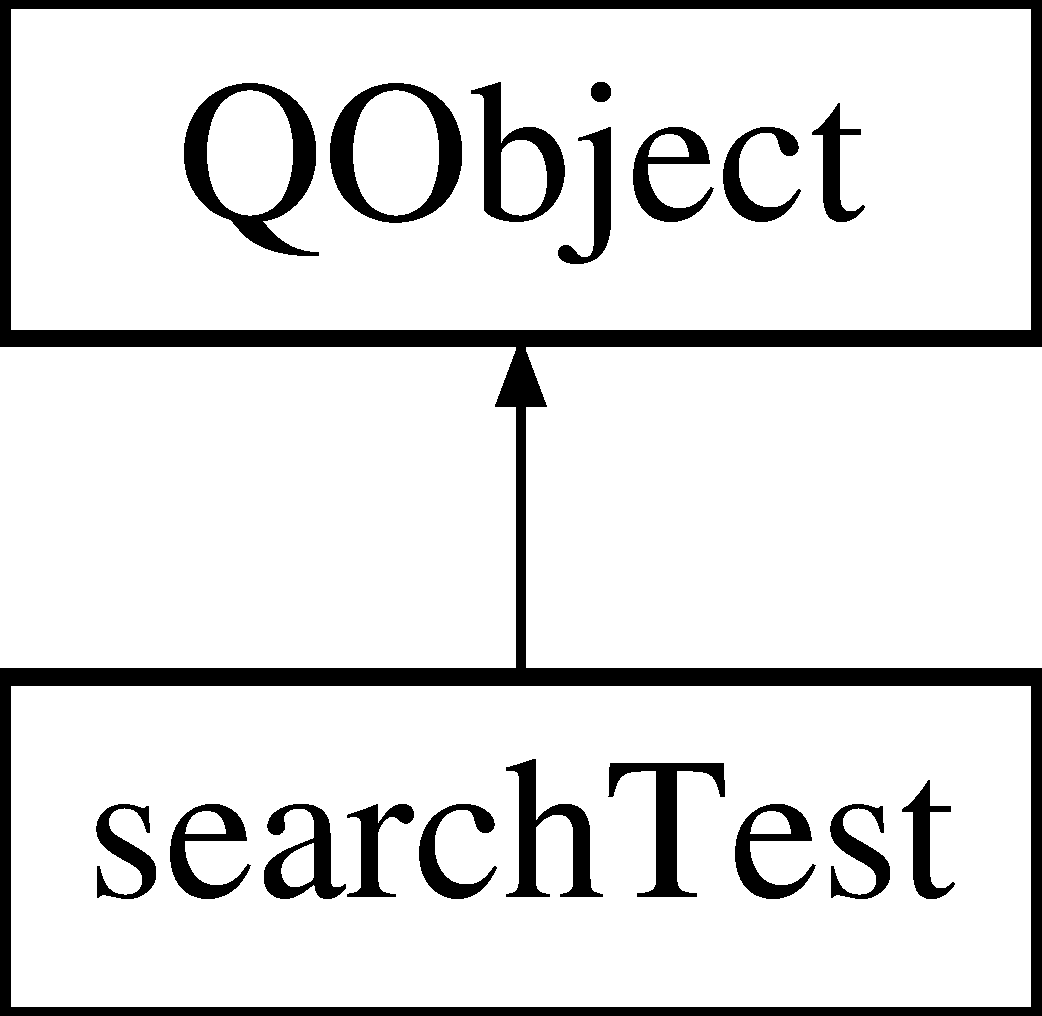
\includegraphics[height=2.000000cm]{d7/d51/classsearchTest}
\end{center}
\end{figure}


The documentation for this class was generated from the following files\+:\begin{DoxyCompactItemize}
\item 
tests/models/searchtest.\+h\item 
tests/models/searchtest.\+cpp\end{DoxyCompactItemize}

\hypertarget{classsearchWidget}{\section{search\-Widget Class Reference}
\label{classsearchWidget}\index{search\-Widget@{search\-Widget}}
}
Inheritance diagram for search\-Widget\-:\begin{figure}[H]
\begin{center}
\leavevmode
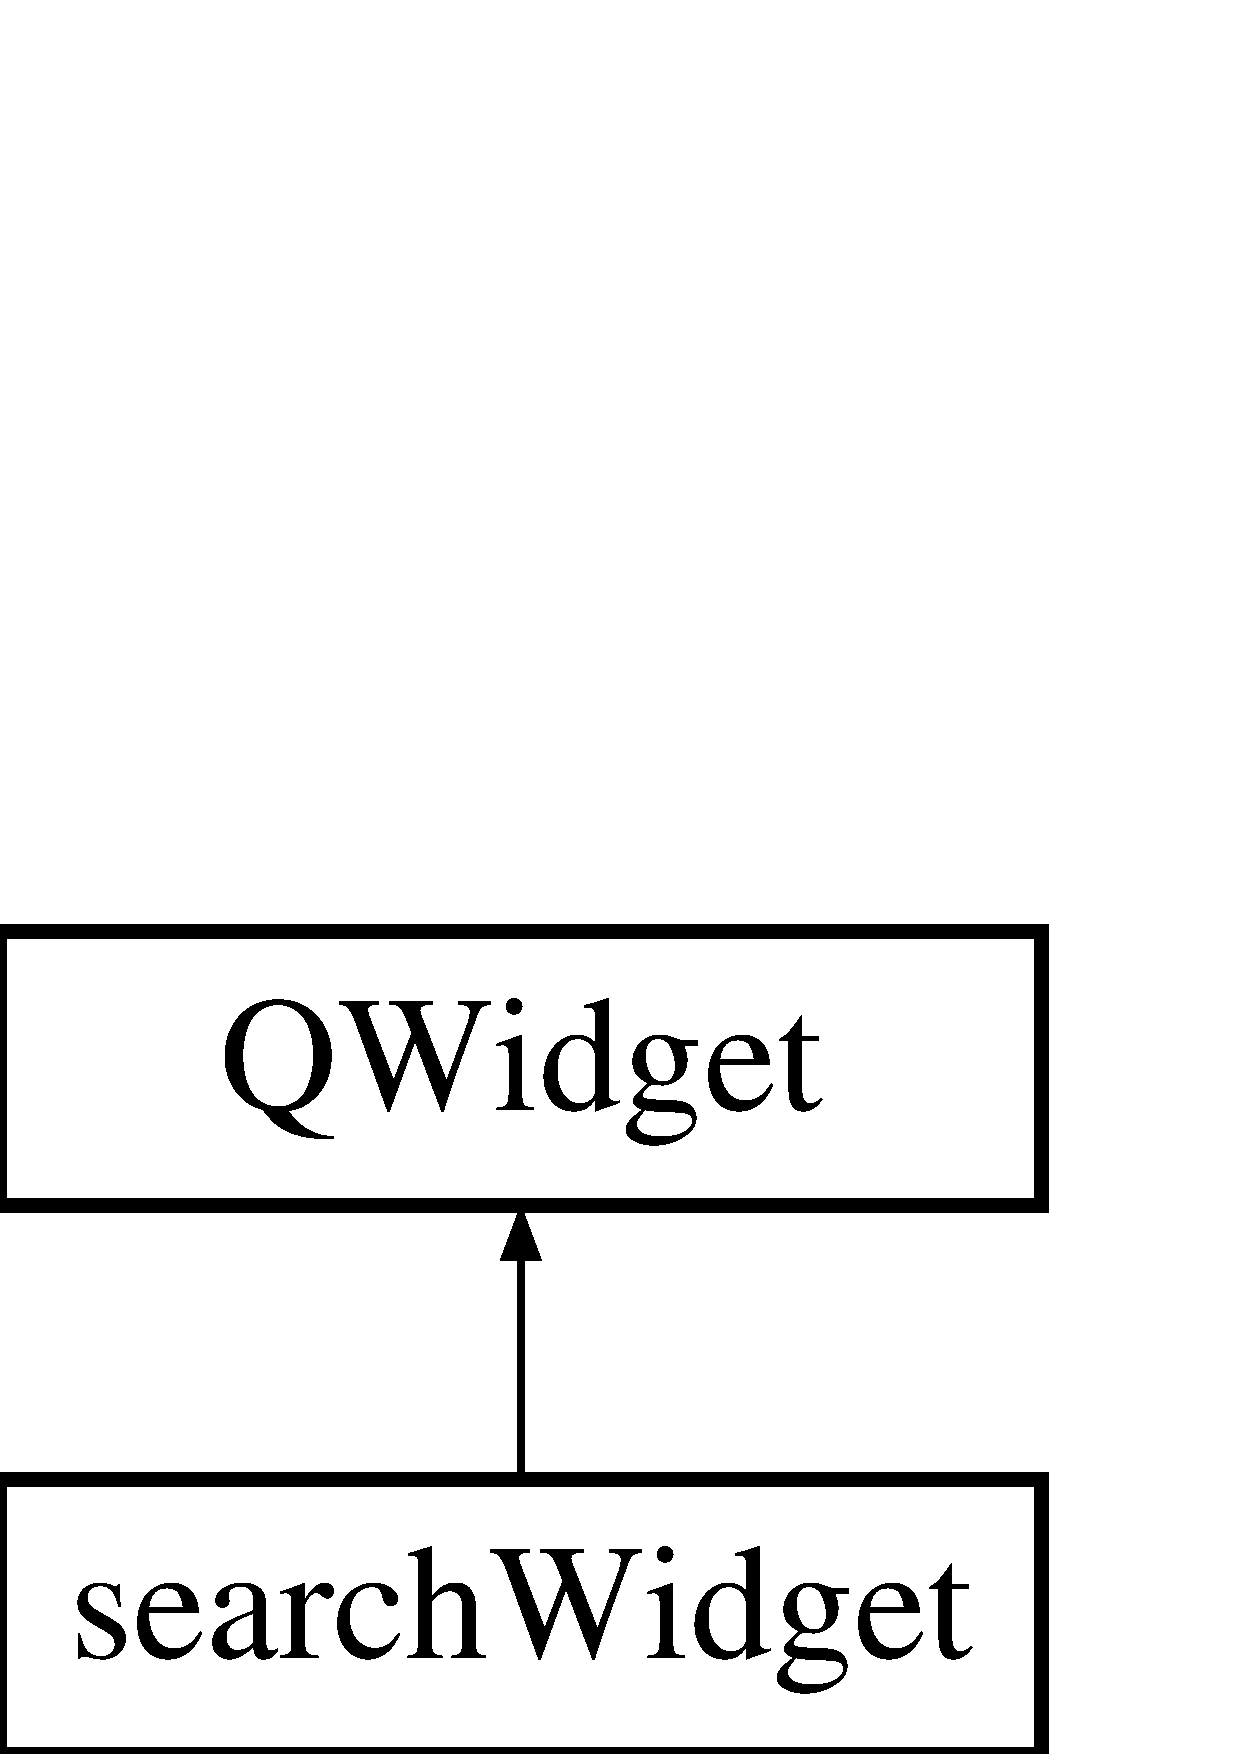
\includegraphics[height=2.000000cm]{d2/dfd/classsearchWidget}
\end{center}
\end{figure}
\subsection*{Public Slots}
\begin{DoxyCompactItemize}
\item 
\hypertarget{classsearchWidget_a01f311627fd5bdbc2886e2dbbe8d7fc7}{void {\bfseries search} (Q\-String)}\label{classsearchWidget_a01f311627fd5bdbc2886e2dbbe8d7fc7}

\end{DoxyCompactItemize}
\subsection*{Public Member Functions}
\begin{DoxyCompactItemize}
\item 
\hypertarget{classsearchWidget_a0c712bf4f3c2105319645ce97e23eba9}{{\bfseries search\-Widget} (Q\-Widget $\ast$parent=0)}\label{classsearchWidget_a0c712bf4f3c2105319645ce97e23eba9}

\item 
int \hyperlink{classsearchWidget_ac74ae97eb8c147c89edc3dec3decf174}{get\-Current\-Customer\-Id} ()
\begin{DoxyCompactList}\small\item\em get\-Current\-Customer\-Id Return the id of the customer selected in the table \end{DoxyCompactList}\end{DoxyCompactItemize}


\subsection{Member Function Documentation}
\hypertarget{classsearchWidget_ac74ae97eb8c147c89edc3dec3decf174}{\index{search\-Widget@{search\-Widget}!get\-Current\-Customer\-Id@{get\-Current\-Customer\-Id}}
\index{get\-Current\-Customer\-Id@{get\-Current\-Customer\-Id}!searchWidget@{search\-Widget}}
\subsubsection[{get\-Current\-Customer\-Id}]{\setlength{\rightskip}{0pt plus 5cm}int search\-Widget\-::get\-Current\-Customer\-Id (
\begin{DoxyParamCaption}
{}
\end{DoxyParamCaption}
)}}\label{classsearchWidget_ac74ae97eb8c147c89edc3dec3decf174}


get\-Current\-Customer\-Id Return the id of the customer selected in the table 

\begin{DoxyReturn}{Returns}
id of the current customer 
\end{DoxyReturn}


The documentation for this class was generated from the following files\-:\begin{DoxyCompactItemize}
\item 
/home/aroquemaurel/projets/qt/\-Fact\-Dev/src/widgets/searchwidget.\-h\item 
/home/aroquemaurel/projets/qt/\-Fact\-Dev/src/widgets/searchwidget.\-cpp\end{DoxyCompactItemize}

\hypertarget{classtestadder}{\section{testadder Class Reference}
\label{classtestadder}\index{testadder@{testadder}}
}


The documentation for this class was generated from the following file\-:\begin{DoxyCompactItemize}
\item 
/home/florent/\-Documents/\-Projet\-\_\-\-S8/\-Fact\-Dev/tests/\-Q\-Test\-Runner/testadder.\-h\end{DoxyCompactItemize}

\hypertarget{classTestAdder}{\section{Test\+Adder$<$ T $>$ Class Template Reference}
\label{classTestAdder}\index{Test\+Adder$<$ T $>$@{Test\+Adder$<$ T $>$}}
}
\subsection*{Public Member Functions}
\begin{DoxyCompactItemize}
\item 
\hypertarget{classTestAdder_a64f9008ae27868e36acdd5c94eebae3b}{{\bfseries Test\+Adder} (const Q\+String \&name)}\label{classTestAdder_a64f9008ae27868e36acdd5c94eebae3b}

\end{DoxyCompactItemize}


The documentation for this class was generated from the following file\+:\begin{DoxyCompactItemize}
\item 
tests/\+Q\+Test\+Runner/testadder.\+cpp\end{DoxyCompactItemize}

\hypertarget{classTestRunner}{\section{Test\-Runner Class Reference}
\label{classTestRunner}\index{Test\-Runner@{Test\-Runner}}
}
\subsection*{Public Member Functions}
\begin{DoxyCompactItemize}
\item 
\hypertarget{classTestRunner_affb5703febccf285914b08ce39e7396f}{{\footnotesize template$<$typename T $>$ }\\char {\bfseries Register\-Test} (Q\-String name)}\label{classTestRunner_affb5703febccf285914b08ce39e7396f}

\item 
\hypertarget{classTestRunner_a10db57abd545dd4f9b93e7aeaae55e4c}{int {\bfseries Run\-All} ()}\label{classTestRunner_a10db57abd545dd4f9b93e7aeaae55e4c}

\end{DoxyCompactItemize}
\subsection*{Static Public Member Functions}
\begin{DoxyCompactItemize}
\item 
\hypertarget{classTestRunner_a4707c4680c85ce622fc375efcf39fc25}{static \hyperlink{classTestRunner}{Test\-Runner} \& {\bfseries Instance} ()}\label{classTestRunner_a4707c4680c85ce622fc375efcf39fc25}

\end{DoxyCompactItemize}


The documentation for this class was generated from the following files\-:\begin{DoxyCompactItemize}
\item 
/home/travis/build/\-F\-A\-C\-T-\/\-Team/\-Fact\-Dev/tests/\-Q\-Test\-Runner/testrunner.\-h\item 
/home/travis/build/\-F\-A\-C\-T-\/\-Team/\-Fact\-Dev/tests/\-Q\-Test\-Runner/testrunner.\-cpp\end{DoxyCompactItemize}

\hypertarget{classUser}{\section{User Class Reference}
\label{classUser}\index{User@{User}}
}


The \hyperlink{classUser}{User} class {\bfseries \hyperlink{classUser}{User}} of it application.  




{\ttfamily \#include $<$user.\-h$>$}

Inheritance diagram for User\-:\begin{figure}[H]
\begin{center}
\leavevmode
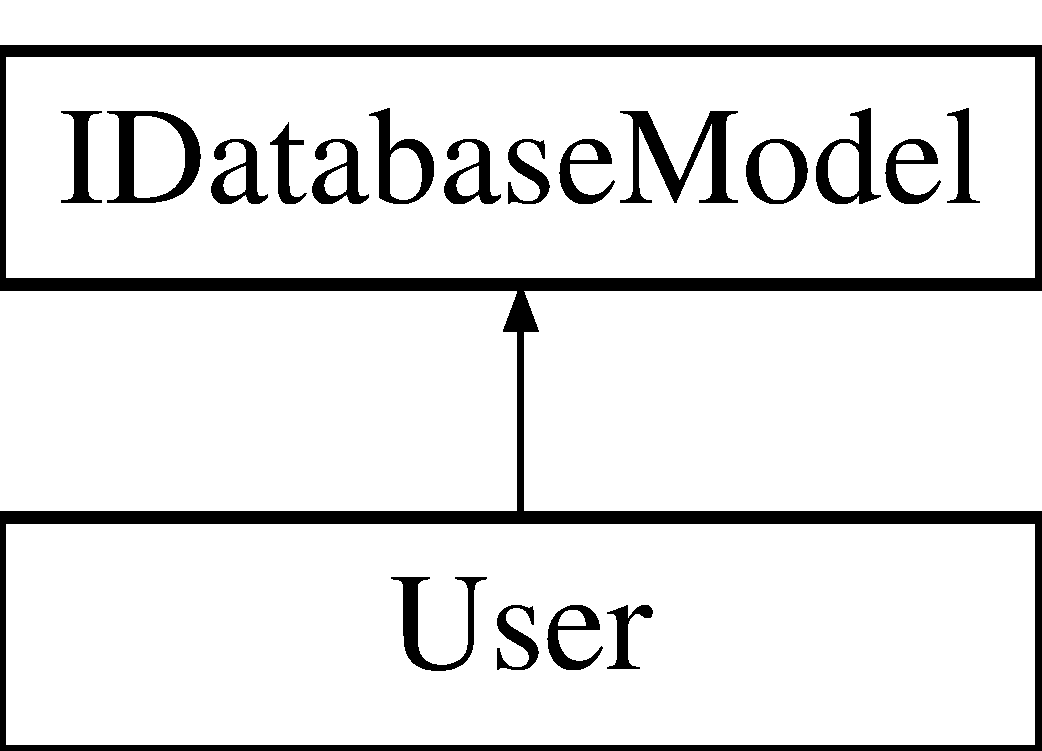
\includegraphics[height=2.000000cm]{d9/dc0/classUser}
\end{center}
\end{figure}
\subsection*{Public Member Functions}
\begin{DoxyCompactItemize}
\item 
\hypertarget{classUser_a4a0137053e591fbb79d9057dd7d2283d}{\hyperlink{classUser_a4a0137053e591fbb79d9057dd7d2283d}{User} ()}\label{classUser_a4a0137053e591fbb79d9057dd7d2283d}

\begin{DoxyCompactList}\small\item\em \hyperlink{classUser_a4a0137053e591fbb79d9057dd7d2283d}{User\-::\-User}. Contruct an \hyperlink{classUser}{User}. \end{DoxyCompactList}\item 
\hyperlink{classUser_a6e84637389bc36a13300df82a7387bb0}{User} (int id)
\begin{DoxyCompactList}\small\item\em \hyperlink{classUser_a4a0137053e591fbb79d9057dd7d2283d}{User\-::\-User}. Construct a \hyperlink{classUser}{User} with the identify {\itshape id} \end{DoxyCompactList}\item 
\hypertarget{classUser_aee39916633f5bf89100a4a917b2db4a2}{void \hyperlink{classUser_aee39916633f5bf89100a4a917b2db4a2}{commit} ()}\label{classUser_aee39916633f5bf89100a4a917b2db4a2}

\begin{DoxyCompactList}\small\item\em \hyperlink{classUser_aee39916633f5bf89100a4a917b2db4a2}{User\-::commit} Update user data in \hyperlink{classUser}{User} table on the database. \end{DoxyCompactList}\item 
void \hyperlink{classUser_a2e4160755d2189979b758929e832b12c}{hydrat} (int id=1)
\begin{DoxyCompactList}\small\item\em \hyperlink{classUser_a2e4160755d2189979b758929e832b12c}{User\-::hydrat} Get data of the user who is specified by {\itshape id} from the database. \end{DoxyCompactList}\item 
\hypertarget{classUser_aba787de7188a5c7bc4b99734b1b093cf}{void \hyperlink{classUser_aba787de7188a5c7bc4b99734b1b093cf}{remove} ()}\label{classUser_aba787de7188a5c7bc4b99734b1b093cf}

\begin{DoxyCompactList}\small\item\em remove Remove the current \hyperlink{classUser}{User} \end{DoxyCompactList}\item 
Q\-String \hyperlink{classUser_acad034d3a093164f056d06d9a3ee33a2}{get\-Firstname} () const 
\begin{DoxyCompactList}\small\item\em \hyperlink{classUser_acad034d3a093164f056d06d9a3ee33a2}{User\-::get\-Firstname} Return the user firstname. \end{DoxyCompactList}\item 
void \hyperlink{classUser_ad9f69006800232eb19146d2354910412}{set\-Firstname} (const Q\-String \&firstname)
\begin{DoxyCompactList}\small\item\em User\-::set\-Firstnament Modify the user {\itshape firstname} \end{DoxyCompactList}\item 
Q\-String \hyperlink{classUser_aabbb05d0c6e6be5ed078ba3c730b24b3}{get\-Lastname} () const 
\begin{DoxyCompactList}\small\item\em \hyperlink{classUser_aabbb05d0c6e6be5ed078ba3c730b24b3}{User\-::get\-Lastname} Return the user lastname. \end{DoxyCompactList}\item 
void \hyperlink{classUser_a90d5bae75aa56253642386ad42da171d}{set\-Lastname} (const Q\-String \&lastname)
\begin{DoxyCompactList}\small\item\em \hyperlink{classUser_a90d5bae75aa56253642386ad42da171d}{User\-::set\-Lastname} Modify the user {\itshape lastname} \end{DoxyCompactList}\item 
Q\-String \hyperlink{classUser_ace35ae55a1681e5df796ebee79fa5b07}{get\-Company} () const 
\begin{DoxyCompactList}\small\item\em \hyperlink{classUser_ace35ae55a1681e5df796ebee79fa5b07}{User\-::get\-Company} Return the user company. \end{DoxyCompactList}\item 
void \hyperlink{classUser_a3a92e61c3e31dddeff27bc8c2307f2db}{set\-Company} (const Q\-String \&company)
\begin{DoxyCompactList}\small\item\em \hyperlink{classUser_a3a92e61c3e31dddeff27bc8c2307f2db}{User\-::set\-Company} Modify the user {\itshape company} name. \end{DoxyCompactList}\item 
Q\-String \hyperlink{classUser_a44af1366445fb0284411f92d37231f2d}{get\-Title} () const 
\begin{DoxyCompactList}\small\item\em \hyperlink{classUser_a44af1366445fb0284411f92d37231f2d}{User\-::get\-Title} Return a short description of \hyperlink{classUser}{User} (company) activity. \end{DoxyCompactList}\item 
void \hyperlink{classUser_ae51847b13715ba1fed59a2778397691a}{set\-Title} (const Q\-String \&title)
\begin{DoxyCompactList}\small\item\em \hyperlink{classUser_ae51847b13715ba1fed59a2778397691a}{User\-::set\-Title} Modify the user/company activities {\itshape description} \end{DoxyCompactList}\item 
Q\-String \hyperlink{classUser_af5cebeb07ba0ebffb916f1f6fd7c002d}{get\-Address} () const 
\begin{DoxyCompactList}\small\item\em \hyperlink{classUser_af5cebeb07ba0ebffb916f1f6fd7c002d}{User\-::get\-Address} Return the company addess (Number and name of street) \end{DoxyCompactList}\item 
void \hyperlink{classUser_a14a70021648f51900cc54f6535d3a603}{set\-Address} (const Q\-String \&address)
\begin{DoxyCompactList}\small\item\em \hyperlink{classUser_a14a70021648f51900cc54f6535d3a603}{User\-::set\-Address} Modify the user company {\itshape address} \end{DoxyCompactList}\item 
Q\-String \hyperlink{classUser_a6a3ecafe2c72860cbc2cfc031d6112c9}{get\-Postal\-Code} () const 
\begin{DoxyCompactList}\small\item\em \hyperlink{classUser_a6a3ecafe2c72860cbc2cfc031d6112c9}{User\-::get\-Postal\-Code} Return the postal code. \end{DoxyCompactList}\item 
void \hyperlink{classUser_af53e170c1701dd1f275589d115f88076}{set\-Postal\-Code} (const Q\-String \&postal\-Code)
\begin{DoxyCompactList}\small\item\em \hyperlink{classUser_af53e170c1701dd1f275589d115f88076}{User\-::set\-Postal\-Code} Modify the postal code {\itshape postal\-Code} \end{DoxyCompactList}\item 
Q\-String \hyperlink{classUser_a78a95519c1fb5ac91152ad231aac1484}{get\-City} () const 
\begin{DoxyCompactList}\small\item\em \hyperlink{classUser_a78a95519c1fb5ac91152ad231aac1484}{User\-::get\-City} Return the city. \end{DoxyCompactList}\item 
void \hyperlink{classUser_a3e350353440e6a22e91c3f78a9a32a4f}{set\-City} (const Q\-String \&city)
\begin{DoxyCompactList}\small\item\em \hyperlink{classUser_a3e350353440e6a22e91c3f78a9a32a4f}{User\-::set\-City} Modify the {\itshape city} \end{DoxyCompactList}\item 
Q\-String \hyperlink{classUser_ae398ada63774cb0c91544637fdd415d1}{get\-Email} () const 
\begin{DoxyCompactList}\small\item\em \hyperlink{classUser_ae398ada63774cb0c91544637fdd415d1}{User\-::get\-Email} Return the user professional {\itshape email} \end{DoxyCompactList}\item 
void \hyperlink{classUser_a13c5e816e990508b469096580884ce98}{set\-Email} (const Q\-String \&email)
\begin{DoxyCompactList}\small\item\em \hyperlink{classUser_a13c5e816e990508b469096580884ce98}{User\-::set\-Email} Modify the user professional {\itshape email} \end{DoxyCompactList}\item 
Q\-String \hyperlink{classUser_a858eff50cbc71969bc5dd5e80045d342}{get\-Mobile\-Phone} () const 
\begin{DoxyCompactList}\small\item\em \hyperlink{classUser_a858eff50cbc71969bc5dd5e80045d342}{User\-::get\-Mobile\-Phone} Return the number of the professional mobile phone. \end{DoxyCompactList}\item 
void \hyperlink{classUser_a8d7afdfc9bcf32b00c20d1d70ae9cbb7}{set\-Mobile\-Phone} (const Q\-String \&mobile\-Phone)
\begin{DoxyCompactList}\small\item\em \hyperlink{classUser_a8d7afdfc9bcf32b00c20d1d70ae9cbb7}{User\-::set\-Mobile\-Phone} Modify the number of the professional user mobile phone {\itshape mobile\-Phone} \end{DoxyCompactList}\item 
Q\-String \hyperlink{classUser_a5408061a1ba87e3d56a51490464d1149}{get\-Phone} () const 
\begin{DoxyCompactList}\small\item\em \hyperlink{classUser_a5408061a1ba87e3d56a51490464d1149}{User\-::get\-Phone} Return the number of the desktop phone. \end{DoxyCompactList}\item 
void \hyperlink{classUser_a271e4179b9da5b409f98656b04431689}{set\-Phone} (const Q\-String \&phone)
\begin{DoxyCompactList}\small\item\em \hyperlink{classUser_a271e4179b9da5b409f98656b04431689}{User\-::set\-Phone} Modify the number of the desktop {\itshape phone} \end{DoxyCompactList}\item 
int \hyperlink{classUser_a721f64ecb20c42c12ca87815ffb0a274}{get\-No\-Siret} () const 
\begin{DoxyCompactList}\small\item\em \hyperlink{classUser_a721f64ecb20c42c12ca87815ffb0a274}{User\-::get\-No\-Siret} Return the S\-I\-R\-E\-T number (company registration number) \end{DoxyCompactList}\item 
void \hyperlink{classUser_a9e77d4724778cfe4f0a6fda75d3b7c52}{set\-No\-Siret} (int no\-Siret)
\begin{DoxyCompactList}\small\item\em \hyperlink{classUser_a9e77d4724778cfe4f0a6fda75d3b7c52}{User\-::set\-No\-Siret} Modify the S\-I\-R\-E\-T number (company registration number) {\itshape no\-Siret} \end{DoxyCompactList}\end{DoxyCompactItemize}
\subsection*{Additional Inherited Members}


\subsection{Detailed Description}
The \hyperlink{classUser}{User} class {\bfseries \hyperlink{classUser}{User}} of it application. 

\begin{DoxyAuthor}{Author}
Florent Berbie 
\end{DoxyAuthor}


\subsection{Constructor \& Destructor Documentation}
\hypertarget{classUser_a6e84637389bc36a13300df82a7387bb0}{\index{User@{User}!User@{User}}
\index{User@{User}!User@{User}}
\subsubsection[{User}]{\setlength{\rightskip}{0pt plus 5cm}User\-::\-User (
\begin{DoxyParamCaption}
\item[{int}]{id}
\end{DoxyParamCaption}
)}}\label{classUser_a6e84637389bc36a13300df82a7387bb0}


\hyperlink{classUser_a4a0137053e591fbb79d9057dd7d2283d}{User\-::\-User}. Construct a \hyperlink{classUser}{User} with the identify {\itshape id} 


\begin{DoxyParams}{Parameters}
{\em id} & \hyperlink{classUser}{User} id \\
\hline
\end{DoxyParams}


\subsection{Member Function Documentation}
\hypertarget{classUser_af5cebeb07ba0ebffb916f1f6fd7c002d}{\index{User@{User}!get\-Address@{get\-Address}}
\index{get\-Address@{get\-Address}!User@{User}}
\subsubsection[{get\-Address}]{\setlength{\rightskip}{0pt plus 5cm}Q\-String User\-::get\-Address (
\begin{DoxyParamCaption}
{}
\end{DoxyParamCaption}
) const}}\label{classUser_af5cebeb07ba0ebffb916f1f6fd7c002d}


\hyperlink{classUser_af5cebeb07ba0ebffb916f1f6fd7c002d}{User\-::get\-Address} Return the company addess (Number and name of street) 

\begin{DoxyReturn}{Returns}
Address company 
\end{DoxyReturn}
\hypertarget{classUser_a78a95519c1fb5ac91152ad231aac1484}{\index{User@{User}!get\-City@{get\-City}}
\index{get\-City@{get\-City}!User@{User}}
\subsubsection[{get\-City}]{\setlength{\rightskip}{0pt plus 5cm}Q\-String User\-::get\-City (
\begin{DoxyParamCaption}
{}
\end{DoxyParamCaption}
) const}}\label{classUser_a78a95519c1fb5ac91152ad231aac1484}


\hyperlink{classUser_a78a95519c1fb5ac91152ad231aac1484}{User\-::get\-City} Return the city. 

\begin{DoxyReturn}{Returns}
city 
\end{DoxyReturn}
\hypertarget{classUser_ace35ae55a1681e5df796ebee79fa5b07}{\index{User@{User}!get\-Company@{get\-Company}}
\index{get\-Company@{get\-Company}!User@{User}}
\subsubsection[{get\-Company}]{\setlength{\rightskip}{0pt plus 5cm}Q\-String User\-::get\-Company (
\begin{DoxyParamCaption}
{}
\end{DoxyParamCaption}
) const}}\label{classUser_ace35ae55a1681e5df796ebee79fa5b07}


\hyperlink{classUser_ace35ae55a1681e5df796ebee79fa5b07}{User\-::get\-Company} Return the user company. 

\begin{DoxyReturn}{Returns}
New company name 
\end{DoxyReturn}
\hypertarget{classUser_ae398ada63774cb0c91544637fdd415d1}{\index{User@{User}!get\-Email@{get\-Email}}
\index{get\-Email@{get\-Email}!User@{User}}
\subsubsection[{get\-Email}]{\setlength{\rightskip}{0pt plus 5cm}Q\-String User\-::get\-Email (
\begin{DoxyParamCaption}
{}
\end{DoxyParamCaption}
) const}}\label{classUser_ae398ada63774cb0c91544637fdd415d1}


\hyperlink{classUser_ae398ada63774cb0c91544637fdd415d1}{User\-::get\-Email} Return the user professional {\itshape email} 

\begin{DoxyReturn}{Returns}
professional email 
\end{DoxyReturn}
\hypertarget{classUser_acad034d3a093164f056d06d9a3ee33a2}{\index{User@{User}!get\-Firstname@{get\-Firstname}}
\index{get\-Firstname@{get\-Firstname}!User@{User}}
\subsubsection[{get\-Firstname}]{\setlength{\rightskip}{0pt plus 5cm}Q\-String User\-::get\-Firstname (
\begin{DoxyParamCaption}
{}
\end{DoxyParamCaption}
) const}}\label{classUser_acad034d3a093164f056d06d9a3ee33a2}


\hyperlink{classUser_acad034d3a093164f056d06d9a3ee33a2}{User\-::get\-Firstname} Return the user firstname. 

\begin{DoxyReturn}{Returns}
\hyperlink{classUser}{User} firstname 
\end{DoxyReturn}
\hypertarget{classUser_aabbb05d0c6e6be5ed078ba3c730b24b3}{\index{User@{User}!get\-Lastname@{get\-Lastname}}
\index{get\-Lastname@{get\-Lastname}!User@{User}}
\subsubsection[{get\-Lastname}]{\setlength{\rightskip}{0pt plus 5cm}Q\-String User\-::get\-Lastname (
\begin{DoxyParamCaption}
{}
\end{DoxyParamCaption}
) const}}\label{classUser_aabbb05d0c6e6be5ed078ba3c730b24b3}


\hyperlink{classUser_aabbb05d0c6e6be5ed078ba3c730b24b3}{User\-::get\-Lastname} Return the user lastname. 

\begin{DoxyReturn}{Returns}
\hyperlink{classUser}{User} lastname 
\end{DoxyReturn}
\hypertarget{classUser_a858eff50cbc71969bc5dd5e80045d342}{\index{User@{User}!get\-Mobile\-Phone@{get\-Mobile\-Phone}}
\index{get\-Mobile\-Phone@{get\-Mobile\-Phone}!User@{User}}
\subsubsection[{get\-Mobile\-Phone}]{\setlength{\rightskip}{0pt plus 5cm}Q\-String User\-::get\-Mobile\-Phone (
\begin{DoxyParamCaption}
{}
\end{DoxyParamCaption}
) const}}\label{classUser_a858eff50cbc71969bc5dd5e80045d342}


\hyperlink{classUser_a858eff50cbc71969bc5dd5e80045d342}{User\-::get\-Mobile\-Phone} Return the number of the professional mobile phone. 

\begin{DoxyReturn}{Returns}
number of mobile phone 
\end{DoxyReturn}
\hypertarget{classUser_a721f64ecb20c42c12ca87815ffb0a274}{\index{User@{User}!get\-No\-Siret@{get\-No\-Siret}}
\index{get\-No\-Siret@{get\-No\-Siret}!User@{User}}
\subsubsection[{get\-No\-Siret}]{\setlength{\rightskip}{0pt plus 5cm}int User\-::get\-No\-Siret (
\begin{DoxyParamCaption}
{}
\end{DoxyParamCaption}
) const}}\label{classUser_a721f64ecb20c42c12ca87815ffb0a274}


\hyperlink{classUser_a721f64ecb20c42c12ca87815ffb0a274}{User\-::get\-No\-Siret} Return the S\-I\-R\-E\-T number (company registration number) 

\begin{DoxyReturn}{Returns}
S\-I\-R\-E\-T number 
\end{DoxyReturn}
\hypertarget{classUser_a5408061a1ba87e3d56a51490464d1149}{\index{User@{User}!get\-Phone@{get\-Phone}}
\index{get\-Phone@{get\-Phone}!User@{User}}
\subsubsection[{get\-Phone}]{\setlength{\rightskip}{0pt plus 5cm}Q\-String User\-::get\-Phone (
\begin{DoxyParamCaption}
{}
\end{DoxyParamCaption}
) const}}\label{classUser_a5408061a1ba87e3d56a51490464d1149}


\hyperlink{classUser_a5408061a1ba87e3d56a51490464d1149}{User\-::get\-Phone} Return the number of the desktop phone. 

\begin{DoxyReturn}{Returns}
number of the desktop phone 
\end{DoxyReturn}
\hypertarget{classUser_a6a3ecafe2c72860cbc2cfc031d6112c9}{\index{User@{User}!get\-Postal\-Code@{get\-Postal\-Code}}
\index{get\-Postal\-Code@{get\-Postal\-Code}!User@{User}}
\subsubsection[{get\-Postal\-Code}]{\setlength{\rightskip}{0pt plus 5cm}Q\-String User\-::get\-Postal\-Code (
\begin{DoxyParamCaption}
{}
\end{DoxyParamCaption}
) const}}\label{classUser_a6a3ecafe2c72860cbc2cfc031d6112c9}


\hyperlink{classUser_a6a3ecafe2c72860cbc2cfc031d6112c9}{User\-::get\-Postal\-Code} Return the postal code. 

\begin{DoxyReturn}{Returns}
postal code 
\end{DoxyReturn}
\hypertarget{classUser_a44af1366445fb0284411f92d37231f2d}{\index{User@{User}!get\-Title@{get\-Title}}
\index{get\-Title@{get\-Title}!User@{User}}
\subsubsection[{get\-Title}]{\setlength{\rightskip}{0pt plus 5cm}Q\-String User\-::get\-Title (
\begin{DoxyParamCaption}
{}
\end{DoxyParamCaption}
) const}}\label{classUser_a44af1366445fb0284411f92d37231f2d}


\hyperlink{classUser_a44af1366445fb0284411f92d37231f2d}{User\-::get\-Title} Return a short description of \hyperlink{classUser}{User} (company) activity. 

\begin{DoxyReturn}{Returns}
a short description of user (company) activity 
\end{DoxyReturn}
\hypertarget{classUser_a2e4160755d2189979b758929e832b12c}{\index{User@{User}!hydrat@{hydrat}}
\index{hydrat@{hydrat}!User@{User}}
\subsubsection[{hydrat}]{\setlength{\rightskip}{0pt plus 5cm}void User\-::hydrat (
\begin{DoxyParamCaption}
\item[{int}]{id = {\ttfamily 1}}
\end{DoxyParamCaption}
)\hspace{0.3cm}{\ttfamily [virtual]}}}\label{classUser_a2e4160755d2189979b758929e832b12c}


\hyperlink{classUser_a2e4160755d2189979b758929e832b12c}{User\-::hydrat} Get data of the user who is specified by {\itshape id} from the database. 


\begin{DoxyParams}{Parameters}
{\em id} & \hyperlink{classUser}{User} identify \\
\hline
\end{DoxyParams}


Implements \hyperlink{classIDatabaseModel}{I\-Database\-Model}.

\hypertarget{classUser_a14a70021648f51900cc54f6535d3a603}{\index{User@{User}!set\-Address@{set\-Address}}
\index{set\-Address@{set\-Address}!User@{User}}
\subsubsection[{set\-Address}]{\setlength{\rightskip}{0pt plus 5cm}void User\-::set\-Address (
\begin{DoxyParamCaption}
\item[{const Q\-String \&}]{address}
\end{DoxyParamCaption}
)}}\label{classUser_a14a70021648f51900cc54f6535d3a603}


\hyperlink{classUser_a14a70021648f51900cc54f6535d3a603}{User\-::set\-Address} Modify the user company {\itshape address} 


\begin{DoxyParams}{Parameters}
{\em address} & Company address (name and number of street) \\
\hline
\end{DoxyParams}
\hypertarget{classUser_a3e350353440e6a22e91c3f78a9a32a4f}{\index{User@{User}!set\-City@{set\-City}}
\index{set\-City@{set\-City}!User@{User}}
\subsubsection[{set\-City}]{\setlength{\rightskip}{0pt plus 5cm}void User\-::set\-City (
\begin{DoxyParamCaption}
\item[{const Q\-String \&}]{city}
\end{DoxyParamCaption}
)}}\label{classUser_a3e350353440e6a22e91c3f78a9a32a4f}


\hyperlink{classUser_a3e350353440e6a22e91c3f78a9a32a4f}{User\-::set\-City} Modify the {\itshape city} 


\begin{DoxyParams}{Parameters}
{\em city} & Company city address \\
\hline
\end{DoxyParams}
\hypertarget{classUser_a3a92e61c3e31dddeff27bc8c2307f2db}{\index{User@{User}!set\-Company@{set\-Company}}
\index{set\-Company@{set\-Company}!User@{User}}
\subsubsection[{set\-Company}]{\setlength{\rightskip}{0pt plus 5cm}void User\-::set\-Company (
\begin{DoxyParamCaption}
\item[{const Q\-String \&}]{company}
\end{DoxyParamCaption}
)}}\label{classUser_a3a92e61c3e31dddeff27bc8c2307f2db}


\hyperlink{classUser_a3a92e61c3e31dddeff27bc8c2307f2db}{User\-::set\-Company} Modify the user {\itshape company} name. 


\begin{DoxyParams}{Parameters}
{\em company} & New user company name \\
\hline
\end{DoxyParams}
\hypertarget{classUser_a13c5e816e990508b469096580884ce98}{\index{User@{User}!set\-Email@{set\-Email}}
\index{set\-Email@{set\-Email}!User@{User}}
\subsubsection[{set\-Email}]{\setlength{\rightskip}{0pt plus 5cm}void User\-::set\-Email (
\begin{DoxyParamCaption}
\item[{const Q\-String \&}]{email}
\end{DoxyParamCaption}
)}}\label{classUser_a13c5e816e990508b469096580884ce98}


\hyperlink{classUser_a13c5e816e990508b469096580884ce98}{User\-::set\-Email} Modify the user professional {\itshape email} 


\begin{DoxyParams}{Parameters}
{\em email} & The user professional email \\
\hline
\end{DoxyParams}
\hypertarget{classUser_ad9f69006800232eb19146d2354910412}{\index{User@{User}!set\-Firstname@{set\-Firstname}}
\index{set\-Firstname@{set\-Firstname}!User@{User}}
\subsubsection[{set\-Firstname}]{\setlength{\rightskip}{0pt plus 5cm}void User\-::set\-Firstname (
\begin{DoxyParamCaption}
\item[{const Q\-String \&}]{firstname}
\end{DoxyParamCaption}
)}}\label{classUser_ad9f69006800232eb19146d2354910412}


User\-::set\-Firstnament Modify the user {\itshape firstname} 


\begin{DoxyParams}{Parameters}
{\em firstname} & New user firstname \\
\hline
\end{DoxyParams}
\hypertarget{classUser_a90d5bae75aa56253642386ad42da171d}{\index{User@{User}!set\-Lastname@{set\-Lastname}}
\index{set\-Lastname@{set\-Lastname}!User@{User}}
\subsubsection[{set\-Lastname}]{\setlength{\rightskip}{0pt plus 5cm}void User\-::set\-Lastname (
\begin{DoxyParamCaption}
\item[{const Q\-String \&}]{lastname}
\end{DoxyParamCaption}
)}}\label{classUser_a90d5bae75aa56253642386ad42da171d}


\hyperlink{classUser_a90d5bae75aa56253642386ad42da171d}{User\-::set\-Lastname} Modify the user {\itshape lastname} 


\begin{DoxyParams}{Parameters}
{\em lastname} & New user lastname \\
\hline
\end{DoxyParams}
\hypertarget{classUser_a8d7afdfc9bcf32b00c20d1d70ae9cbb7}{\index{User@{User}!set\-Mobile\-Phone@{set\-Mobile\-Phone}}
\index{set\-Mobile\-Phone@{set\-Mobile\-Phone}!User@{User}}
\subsubsection[{set\-Mobile\-Phone}]{\setlength{\rightskip}{0pt plus 5cm}void User\-::set\-Mobile\-Phone (
\begin{DoxyParamCaption}
\item[{const Q\-String \&}]{mobile\-Phone}
\end{DoxyParamCaption}
)}}\label{classUser_a8d7afdfc9bcf32b00c20d1d70ae9cbb7}


\hyperlink{classUser_a8d7afdfc9bcf32b00c20d1d70ae9cbb7}{User\-::set\-Mobile\-Phone} Modify the number of the professional user mobile phone {\itshape mobile\-Phone} 


\begin{DoxyParams}{Parameters}
{\em mobile\-Phone} & Number of the professional mobile phone \\
\hline
\end{DoxyParams}
\hypertarget{classUser_a9e77d4724778cfe4f0a6fda75d3b7c52}{\index{User@{User}!set\-No\-Siret@{set\-No\-Siret}}
\index{set\-No\-Siret@{set\-No\-Siret}!User@{User}}
\subsubsection[{set\-No\-Siret}]{\setlength{\rightskip}{0pt plus 5cm}void User\-::set\-No\-Siret (
\begin{DoxyParamCaption}
\item[{int}]{no\-Siret}
\end{DoxyParamCaption}
)}}\label{classUser_a9e77d4724778cfe4f0a6fda75d3b7c52}


\hyperlink{classUser_a9e77d4724778cfe4f0a6fda75d3b7c52}{User\-::set\-No\-Siret} Modify the S\-I\-R\-E\-T number (company registration number) {\itshape no\-Siret} 


\begin{DoxyParams}{Parameters}
{\em no\-Siret} & S\-I\-R\-E\-T number \\
\hline
\end{DoxyParams}
\hypertarget{classUser_a271e4179b9da5b409f98656b04431689}{\index{User@{User}!set\-Phone@{set\-Phone}}
\index{set\-Phone@{set\-Phone}!User@{User}}
\subsubsection[{set\-Phone}]{\setlength{\rightskip}{0pt plus 5cm}void User\-::set\-Phone (
\begin{DoxyParamCaption}
\item[{const Q\-String \&}]{phone}
\end{DoxyParamCaption}
)}}\label{classUser_a271e4179b9da5b409f98656b04431689}


\hyperlink{classUser_a271e4179b9da5b409f98656b04431689}{User\-::set\-Phone} Modify the number of the desktop {\itshape phone} 


\begin{DoxyParams}{Parameters}
{\em phone} & Number of the desktop phone \\
\hline
\end{DoxyParams}
\hypertarget{classUser_af53e170c1701dd1f275589d115f88076}{\index{User@{User}!set\-Postal\-Code@{set\-Postal\-Code}}
\index{set\-Postal\-Code@{set\-Postal\-Code}!User@{User}}
\subsubsection[{set\-Postal\-Code}]{\setlength{\rightskip}{0pt plus 5cm}void User\-::set\-Postal\-Code (
\begin{DoxyParamCaption}
\item[{const Q\-String \&}]{postal\-Code}
\end{DoxyParamCaption}
)}}\label{classUser_af53e170c1701dd1f275589d115f88076}


\hyperlink{classUser_af53e170c1701dd1f275589d115f88076}{User\-::set\-Postal\-Code} Modify the postal code {\itshape postal\-Code} 


\begin{DoxyParams}{Parameters}
{\em postal\-Code} & New postal code \\
\hline
\end{DoxyParams}
\hypertarget{classUser_ae51847b13715ba1fed59a2778397691a}{\index{User@{User}!set\-Title@{set\-Title}}
\index{set\-Title@{set\-Title}!User@{User}}
\subsubsection[{set\-Title}]{\setlength{\rightskip}{0pt plus 5cm}void User\-::set\-Title (
\begin{DoxyParamCaption}
\item[{const Q\-String \&}]{title}
\end{DoxyParamCaption}
)}}\label{classUser_ae51847b13715ba1fed59a2778397691a}


\hyperlink{classUser_ae51847b13715ba1fed59a2778397691a}{User\-::set\-Title} Modify the user/company activities {\itshape description} 


\begin{DoxyParams}{Parameters}
{\em title} & Short description on activity(ies) of customer company \\
\hline
\end{DoxyParams}


The documentation for this class was generated from the following files\-:\begin{DoxyCompactItemize}
\item 
/home/florent/\-Documents/\-Projet\-\_\-\-S8/\-Fact\-Dev/src/models/user.\-h\item 
/home/florent/\-Documents/\-Projet\-\_\-\-S8/\-Fact\-Dev/src/models/user.\-cpp\end{DoxyCompactItemize}

\hypertarget{classUserDatabase}{\section{User\-Database Class Reference}
\label{classUserDatabase}\index{User\-Database@{User\-Database}}
}


The \hyperlink{classUserDatabase}{User\-Database} class Access to \hyperlink{classUser}{User} data in the the table \hyperlink{classUser}{User} of the {\bfseries \hyperlink{classDatabase}{Database}}  




{\ttfamily \#include $<$userdatabase.\-h$>$}

Inheritance diagram for User\-Database\-:\begin{figure}[H]
\begin{center}
\leavevmode
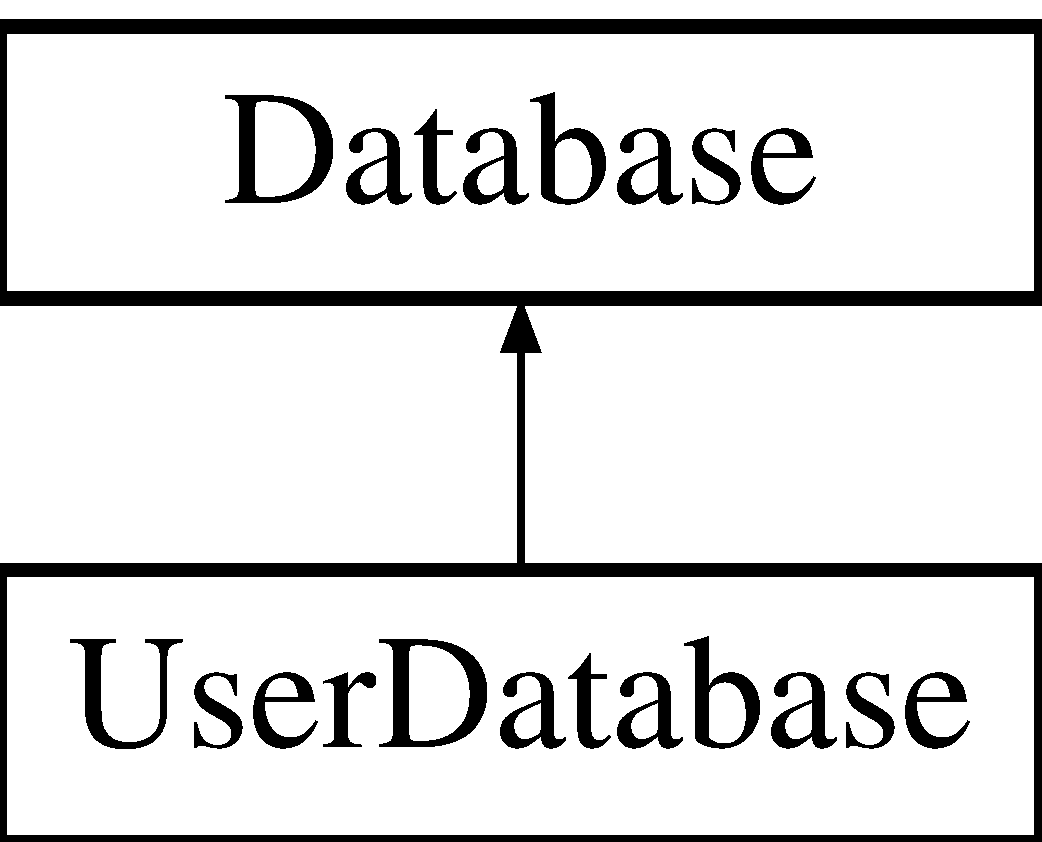
\includegraphics[height=2.000000cm]{de/d47/classUserDatabase}
\end{center}
\end{figure}
\subsection*{Public Member Functions}
\begin{DoxyCompactItemize}
\item 
Q\-Standard\-Item\-Model $\ast$ \hyperlink{classUserDatabase_a6020d6686916f20b3e6a1a5fa5fa7978}{get\-User\-Table} ()  throw (\-Db\-Exception$\ast$)
\begin{DoxyCompactList}\small\item\em get\-User\-Table Return an item model of \hyperlink{classUser}{User} for Q\-Table\-View \end{DoxyCompactList}\item 
\hyperlink{classUser}{User} $\ast$ \hyperlink{classUserDatabase_ab95ed012ce83d09e57ad902cc304585c}{get\-User} (const int p\-Id=1)
\begin{DoxyCompactList}\small\item\em get\-User Get informations about the user (identified by 'p\-Id') \end{DoxyCompactList}\item 
\hypertarget{classUserDatabase_a5d7ecaa321c764615ed3cff211ccd84f}{void \hyperlink{classUserDatabase_a5d7ecaa321c764615ed3cff211ccd84f}{update\-User} (const \hyperlink{classUser}{User} \&)}\label{classUserDatabase_a5d7ecaa321c764615ed3cff211ccd84f}

\begin{DoxyCompactList}\small\item\em update\-User Update informations about the user \end{DoxyCompactList}\end{DoxyCompactItemize}
\subsection*{Static Public Member Functions}
\begin{DoxyCompactItemize}
\item 
static \hyperlink{classUserDatabase}{User\-Database} $\ast$ \hyperlink{classUserDatabase_aa1ce356d9f6f903c786e5f623dac90b6}{instance} ()  throw (\-Db\-Exception$\ast$)
\begin{DoxyCompactList}\small\item\em User\-Database\-::get\-Instance Return an instance of \hyperlink{classUserDatabase}{User\-Database}. \end{DoxyCompactList}\end{DoxyCompactItemize}
\subsection*{Additional Inherited Members}


\subsection{Detailed Description}
The \hyperlink{classUserDatabase}{User\-Database} class Access to \hyperlink{classUser}{User} data in the the table \hyperlink{classUser}{User} of the {\bfseries \hyperlink{classDatabase}{Database}} 

\begin{DoxyAuthor}{Author}
Florent Berbie 
\end{DoxyAuthor}
\begin{DoxySeeAlso}{See Also}
\hyperlink{classDatabase}{Database} 

\hyperlink{classUser}{User} 
\end{DoxySeeAlso}


\subsection{Member Function Documentation}
\hypertarget{classUserDatabase_ab95ed012ce83d09e57ad902cc304585c}{\index{User\-Database@{User\-Database}!get\-User@{get\-User}}
\index{get\-User@{get\-User}!UserDatabase@{User\-Database}}
\subsubsection[{get\-User}]{\setlength{\rightskip}{0pt plus 5cm}{\bf User} $\ast$ User\-Database\-::get\-User (
\begin{DoxyParamCaption}
\item[{const int}]{p\-Id = {\ttfamily 1}}
\end{DoxyParamCaption}
)}}\label{classUserDatabase_ab95ed012ce83d09e57ad902cc304585c}


get\-User Get informations about the user (identified by 'p\-Id') 


\begin{DoxyParams}{Parameters}
{\em p\-Id} & user id (1 default) $\ast$ \\
\hline
\end{DoxyParams}
\begin{DoxyReturn}{Returns}
the user 
\end{DoxyReturn}
\hypertarget{classUserDatabase_a6020d6686916f20b3e6a1a5fa5fa7978}{\index{User\-Database@{User\-Database}!get\-User\-Table@{get\-User\-Table}}
\index{get\-User\-Table@{get\-User\-Table}!UserDatabase@{User\-Database}}
\subsubsection[{get\-User\-Table}]{\setlength{\rightskip}{0pt plus 5cm}Q\-Standard\-Item\-Model$\ast$ User\-Database\-::get\-User\-Table (
\begin{DoxyParamCaption}
{}
\end{DoxyParamCaption}
) throw  {\bf Db\-Exception} $\ast$) }}\label{classUserDatabase_a6020d6686916f20b3e6a1a5fa5fa7978}


get\-User\-Table Return an item model of \hyperlink{classUser}{User} for Q\-Table\-View 

\begin{DoxyReturn}{Returns}
Q\-Standard\-Item\-Model an item model 
\end{DoxyReturn}
\hypertarget{classUserDatabase_aa1ce356d9f6f903c786e5f623dac90b6}{\index{User\-Database@{User\-Database}!instance@{instance}}
\index{instance@{instance}!UserDatabase@{User\-Database}}
\subsubsection[{instance}]{\setlength{\rightskip}{0pt plus 5cm}{\bf User\-Database} $\ast$ User\-Database\-::instance (
\begin{DoxyParamCaption}
{}
\end{DoxyParamCaption}
) throw  {\bf Db\-Exception} $\ast$) \hspace{0.3cm}{\ttfamily [static]}}}\label{classUserDatabase_aa1ce356d9f6f903c786e5f623dac90b6}


User\-Database\-::get\-Instance Return an instance of \hyperlink{classUserDatabase}{User\-Database}. 

\begin{DoxyReturn}{Returns}
Instance of \hyperlink{classUserDatabase}{User\-Database} 
\end{DoxyReturn}


The documentation for this class was generated from the following files\-:\begin{DoxyCompactItemize}
\item 
/home/florent/\-Documents/\-Projet\-\_\-\-S8/\-Fact\-Dev/src/database/userdatabase.\-h\item 
/home/florent/\-Documents/\-Projet\-\_\-\-S8/\-Fact\-Dev/src/database/userdatabase.\-cpp\end{DoxyCompactItemize}

\hypertarget{classUserDataDialog}{\section{User\-Data\-Dialog Class Reference}
\label{classUserDataDialog}\index{User\-Data\-Dialog@{User\-Data\-Dialog}}
}


The \hyperlink{classUserDataDialog}{User\-Data\-Dialog} class Window to fill user data.  




{\ttfamily \#include $<$userdatadialog.\-h$>$}

Inheritance diagram for User\-Data\-Dialog\-:\begin{figure}[H]
\begin{center}
\leavevmode
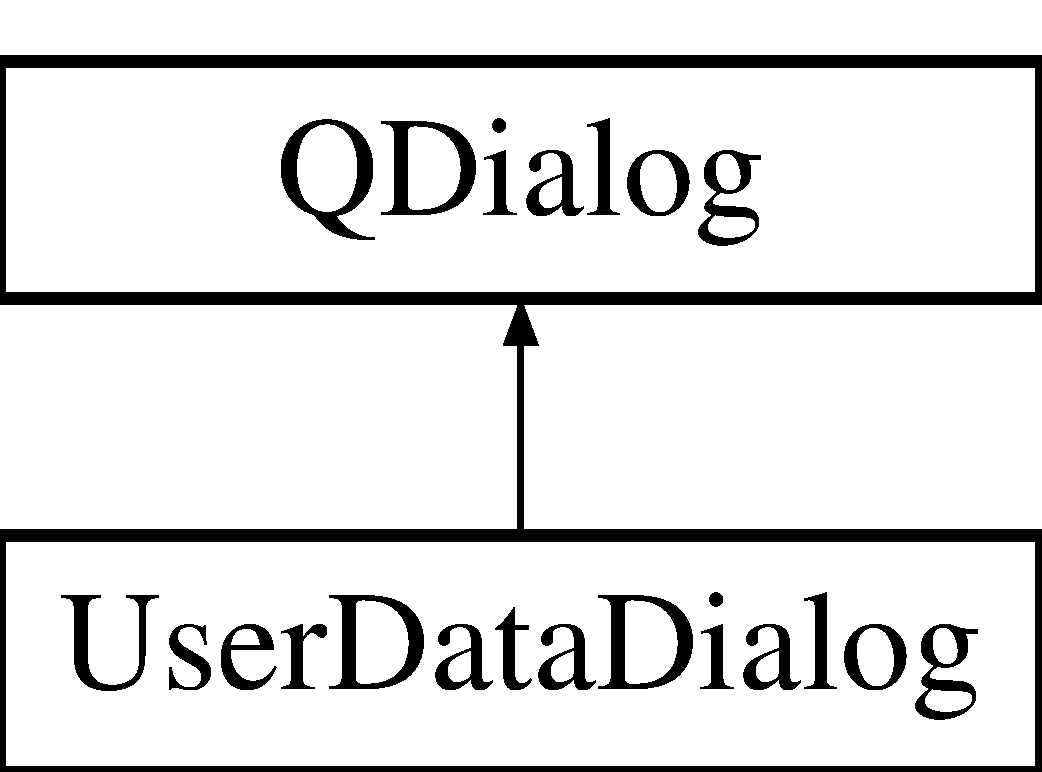
\includegraphics[height=2.000000cm]{de/d9c/classUserDataDialog}
\end{center}
\end{figure}
\subsection*{Public Member Functions}
\begin{DoxyCompactItemize}
\item 
\hyperlink{classUserDataDialog_a51210d5e027d49b019fcd565d5b20e06}{User\-Data\-Dialog} (Q\-Widget $\ast$parent=0)
\begin{DoxyCompactList}\small\item\em \hyperlink{classUserDataDialog}{User\-Data\-Dialog}\-: Construct a window with user data. \end{DoxyCompactList}\item 
\hypertarget{classUserDataDialog_a22f266169243757212ba7eb61d083ddb}{void \hyperlink{classUserDataDialog_a22f266169243757212ba7eb61d083ddb}{fill\-Fields} ()}\label{classUserDataDialog_a22f266169243757212ba7eb61d083ddb}

\begin{DoxyCompactList}\small\item\em \hyperlink{classUserDataDialog_a22f266169243757212ba7eb61d083ddb}{User\-Data\-Dialog\-::fill\-Fields} Fill line edits with the data of the user. \end{DoxyCompactList}\item 
\hypertarget{classUserDataDialog_ad6ba344db1a10b804ca8f5f9a6ffed2c}{void \hyperlink{classUserDataDialog_ad6ba344db1a10b804ca8f5f9a6ffed2c}{accept} ()}\label{classUserDataDialog_ad6ba344db1a10b804ca8f5f9a6ffed2c}

\begin{DoxyCompactList}\small\item\em accept Valid data inputed by user and add these data in \hyperlink{classDatabase}{Database} \end{DoxyCompactList}\item 
\hypertarget{classUserDataDialog_a54519d6441212d50849de7b72ac5e623}{void \hyperlink{classUserDataDialog_a54519d6441212d50849de7b72ac5e623}{reject} ()}\label{classUserDataDialog_a54519d6441212d50849de7b72ac5e623}

\begin{DoxyCompactList}\small\item\em reject Cancel the operation and close the windows \end{DoxyCompactList}\end{DoxyCompactItemize}


\subsection{Detailed Description}
The \hyperlink{classUserDataDialog}{User\-Data\-Dialog} class Window to fill user data. 

\begin{DoxyAuthor}{Author}
Florent Berbie 
\end{DoxyAuthor}


\subsection{Constructor \& Destructor Documentation}
\hypertarget{classUserDataDialog_a51210d5e027d49b019fcd565d5b20e06}{\index{User\-Data\-Dialog@{User\-Data\-Dialog}!User\-Data\-Dialog@{User\-Data\-Dialog}}
\index{User\-Data\-Dialog@{User\-Data\-Dialog}!UserDataDialog@{User\-Data\-Dialog}}
\subsubsection[{User\-Data\-Dialog}]{\setlength{\rightskip}{0pt plus 5cm}User\-Data\-Dialog\-::\-User\-Data\-Dialog (
\begin{DoxyParamCaption}
\item[{Q\-Widget $\ast$}]{parent = {\ttfamily 0}}
\end{DoxyParamCaption}
)\hspace{0.3cm}{\ttfamily [explicit]}}}\label{classUserDataDialog_a51210d5e027d49b019fcd565d5b20e06}


\hyperlink{classUserDataDialog}{User\-Data\-Dialog}\-: Construct a window with user data. 


\begin{DoxyParams}{Parameters}
{\em parent} & \\
\hline
\end{DoxyParams}


The documentation for this class was generated from the following files\-:\begin{DoxyCompactItemize}
\item 
/home/florent/\-Documents/\-Projet\-\_\-\-S8/\-Fact\-Dev/src/dialogs/userdatadialog.\-h\item 
/home/florent/\-Documents/\-Projet\-\_\-\-S8/\-Fact\-Dev/src/dialogs/userdatadialog.\-cpp\end{DoxyCompactItemize}

\hypertarget{classUtils}{\section{Utils Class Reference}
\label{classUtils}\index{Utils@{Utils}}
}


The \hyperlink{classUtils}{Utils} class.  




{\ttfamily \#include $<$utils.\+h$>$}

\subsection*{Static Public Member Functions}
\begin{DoxyCompactItemize}
\item 
static Q\+String \hyperlink{classUtils_a009b2a8ef00831aff87d2e46ca209398}{first\+Letter\+To\+Upper} (Q\+String s)
\begin{DoxyCompactList}\small\item\em first\+Letter\+To\+Upper Put the first letter of a string in capslock \end{DoxyCompactList}\end{DoxyCompactItemize}


\subsection{Detailed Description}
The \hyperlink{classUtils}{Utils} class. 

\begin{DoxyAuthor}{Author}
Antoine de Roquemaurel 
\end{DoxyAuthor}


\subsection{Member Function Documentation}
\hypertarget{classUtils_a009b2a8ef00831aff87d2e46ca209398}{\index{Utils@{Utils}!first\+Letter\+To\+Upper@{first\+Letter\+To\+Upper}}
\index{first\+Letter\+To\+Upper@{first\+Letter\+To\+Upper}!Utils@{Utils}}
\subsubsection[{first\+Letter\+To\+Upper}]{\setlength{\rightskip}{0pt plus 5cm}Q\+String Utils\+::first\+Letter\+To\+Upper (
\begin{DoxyParamCaption}
\item[{Q\+String}]{s}
\end{DoxyParamCaption}
)\hspace{0.3cm}{\ttfamily [static]}}}\label{classUtils_a009b2a8ef00831aff87d2e46ca209398}


first\+Letter\+To\+Upper Put the first letter of a string in capslock 


\begin{DoxyParams}{Parameters}
{\em s} & The string to display \\
\hline
\end{DoxyParams}
\begin{DoxyReturn}{Returns}
The new string with caps 
\end{DoxyReturn}


The documentation for this class was generated from the following files\+:\begin{DoxyCompactItemize}
\item 
src/utils.\+h\item 
src/utils.\+cpp\end{DoxyCompactItemize}

%--- End generated contents ---

% Index
\newpage
\phantomsection
\addcontentsline{toc}{chapter}{Index}
\printindex

\end{document}
